\documentclass[%
candidate,   % тип документа
natbib,      % использовать пакет natbib для "сжатия" цитирований
subf,        % использовать пакет subcaption для вложенной нумерации рисунков
href,        % использовать пакет hyperref для создания гиперссылок
colorlinks,  % цветные гиперссылки
%fixint,     % включить прямые знаки интегралов
%classified, % гриф секретности
%facsimile,  % отображать факсимиле диссертанта
]{disser}

\usepackage[
  a4paper, mag=1000,
  left=2.5cm, right=1cm, top=2cm, bottom=2cm, headsep=0.7cm, footskip=1cm
]{geometry}

%\usepackage{tocloft}
\usepackage[intlimits]{amsmath}
\usepackage{amssymb,amsfonts}

\usepackage[T2A]{fontenc}
\usepackage[cp1251]{inputenc}
\usepackage[english,russian]{babel}
\usepackage{epsfig}
\ifpdf\usepackage{epstopdf}\fi
\usepackage[autostyle]{csquotes}
%\usepackage{doctor}

% Список сокращений и условных обозначений
\usepackage[intoc,nocfg,russian]{nomencl}
\newcommand{\nomencl}[2]{#1 --- #2\nomenclature{#1}{#2}}
\setlength{\nomlabelwidth}{3em}
\setlength{\nomitemsep}{-\parsep}
\setcounter{tocdepth}{2}
\renewcommand{\nomlabel}[1]{#1 ---}
\makenomenclature

% Шрифт Times в тексте как основной
%\usepackage{tempora}
% альтернативный пакет из дистрибутива TeX Live
%\usepackage{cyrtimes}

% Шрифт Times в формулах как основной
%\usepackage[varg,cmbraces,cmintegrals]{newtxmath}
% альтернативный пакет
%\usepackage[subscriptcorrection,nofontinfo]{mtpro2}

% Плавающие рисунки "в оборку".
\usepackage{wrapfig}

% Номера страниц снизу и по центру
%\pagestyle{footcenter}
%\chapterpagestyle{footcenter}

% Точка с запятой в качестве разделителя между номерами цитирований
%\setcitestyle{semicolon}

% Ссылки на работы соискателя включаются в общий список литературы
\let\citeown=\cite

% Использовать полужирное начертание для векторов
\let\vec=\mathbf

% Путь к файлам с иллюстрациями
\graphicspath{{fig/}}
\def\mprp{\mbox{\tiny $\bot$}}
\def\mprl{\mbox{\tiny $\|$}}
\def\th{\mbox{th}}

\def\D{\mathrm{d}}
\def\beq{\begin{eqnarray}}
\def\eeq{\end{eqnarray}}
\def\ee{\varepsilon}
\def\lm{\lambda}
\newcommand{\prp}[1]{#1_{\mbox{\tiny $\bot$}}}
\newcommand{\pprl}[1]{#1_{\mbox{\tiny $\|$}}}
\newcommand{\ii}{\mathrm{i}} % мнимая единица
\newcommand{\dd}{\mathrm{d}} % дифференциал
\newcommand{\eee}{\mathrm{e}} % основание натуральных логарифмов
\def\HH{H\!\!\left(\frac{4 m^2}{\pprl{q}^2}\right)}
\def\HHi{H\!\!\left(\frac{4 m^2}{\pprl{q'^2}}\right)}
\def\HHii{H\!\!\left(\frac{4 m^2}{\pprl{q''^2}}\right)}
\def\ggg{\gamma \rightarrow \gamma \gamma}
\def\ff{\Lambda}
\def\tff{\widetilde \Lambda}
\def\1{1 \to 1 \, 2}
\def\2{1 \to 2 \, 2}
\def\S{{\cal S}}
\def\J{{\cal J}}
\def\A{{\cal A}}
\def\P{{\cal P}}
\def\M{{\cal M}}
\newcommand{\bs}{\boldsymbol} 

\def\changemargin#1#2{\list{}{\rightmargin#2\leftmargin#1}\item[]}
\let\endchangemargin=\endlist 

\begin{document}

% Переопределение стандартных заголовков
%\def\contentsname{Содержание}
%\def\conclusionname{Выводы}
%\def\bibname{Литература}

% Включение файла с общим текстом диссертации и автореферата
% (текст титульного листа и характеристика работы).
% ����� ���� ���������� ����� ����������� � ������������
\institution{����������� ��������������� ��������� ��������������� ���������� ������� �����������\\ 
������������ ��������������� ����������� ��. �.�. ��������}

\topic{��������� � ���������������� ��������� ��������� �� ������� �������� �����}

\author{����� ������� �����������}

\specnum{1.3.3}
\spec{������������� ������}

\sa{�������� ������� �������������}
\sastatus{������~���.-���.~����}

\city{���������}
\date{\number\year}


% номер копии для грифа секретности
%\copynum{1}
% класс доступа
%\classlabel{Для служебного пользования}

% номер УДК
%\libcatnum{12345}

\title{ДИССЕРТАЦИЯ\\
на соискание ученой степени\\
кандидата физико-математических наук}

\maketitle

%%
%% Titlepage in English
%%
%
%\institution{Name of Organization}
%
%\title{PhD Thesis}
%
%% Topic
%\topic{Dummy Title}
%
%% Author
%\author{Author's Name}
%
%\specnum{01.04.05}
%\spec{Optics}
%
%%\specsndnum{01.04.07}
%%\specsnd{Condensed matter physics}
%
%\sa{I.\,I.~Ivanov}
%\sastatus{Professor}
%%\sasnd{P.\,P.~Petrov}
%%\sasndstatus{Professor}
%
%% Scientific consultant
%%\scon{B.\,B.~Baranov}
%%\sconstatus{Professor}
%
%% City & Year
%\city{Saint Petersburg}
%\date{\number\year}
%
%\maketitle[en]

\tableofcontents
% ����� ������� ������������ � �����������
\mkcommonsect{actuality}{������������ ���� ������������.}{%
	���������� ������, ������� ������� ������������� �������������, �������� ���������� ����������� ������������� � ������ �� ����� ���������� ��������, ��������� � �����. 
	������ �������� ������ ���������� �������, ���������� ���������� ������ ������������ �������������, � �������� ������� ����� ������ ������������ � ������ ��������. � ���������� ���� ������� ����������� ��������, ���������� ����������� ��� ������� ����������� ������� ��������� ����� ������� ����� $B_e = m^2 / e \simeq 4.41 \times 10^{13}$ ��, ��� $e>0$ -- ������������ ����� ���������, \linebreak $m$ -- ����� ���������.  ��� ����������� �������� ������������� ���������� ���� � ������������  ���������� ����������� ��������� ���������� ��������� ������� ��� �������� � ��� ������. � ������ �������, ����������� ������������� ���� $E=m^2/e$ �������� ����������, ��� ��� ���� ������ �������� �������� � ������������ �������� ��������-����������� ���, �������� �����������  ������� ���� �������� ��� � ����������� ������~\cite{Schwinger:1951}, ������� ����� ������������� ���� ����� �������� �������� ��������. ������,\linebreak ��� ���� �������� � ������~\cite{KM_Book_2013}, ��������� ����, � ���� ������������ �������, ����� ��������� ����������� �������� � ���� ������ ��������������� ����, ���� ��� ���������� ��������������� ��������������, ������� � ����� ������������ ����� ��������� ����������� ��������. ����� �������  ��-�������� ����������� � �������������� � ����������.
	
	������������� -- ��� ����������������� ��������� ���������� ������, ������� ������������� ������������� ��������� � �������������� ��������� ����������������� ������� �� ���������� ��������. �������� ����������� �������~\cite{Gunn:1969,Pacini:1970} �������� ���������� ������ ������� �������� ��� �������������� � ��������� �������� $P<2$ c �������� �������-��������� ���������. ������ �� �����, ���� �������� ������ ��������� ����� �� ����������� ��������������~\cite{Kim:2023}: $B\sim 10^{10}-10^{14}$ �� ��� ������������������� ($0.1\text{ �}<P<2$~�) ��������� � $B\sim10^8-10^{14}$~�� ��� �������������������� ($P<0.1$ �). ����� 110 �� 1468 �������������� � ������~\cite{Kim:2023} �������� �������� ���������� ������ ������� ������������ ��������, �������� ��� ������ �� ��� ������������� �������� ������������� ���������� ���� $B\simeq7.56 \times 10^{14}$~��. ������ �������� ����� �������������� ������� ��������� ���� ��������� � �������� ���������� �������, ��� �������� � ��������� ����������������� ���������.    �������� �� ���������� ������ ���������� ��������������, �� �������������� �������� ���������� ��������, ���� �� ��������� ���������� �������� ������������, ��������, � ������~\cite{Philippov_2020}.
	
	������� ��������� � ������, �������� ������������ ��������, �������� ������������� �������� -- ������ ������������� ���������� ������, ����������� � ������ ������� ������� � ������� �������. ���������� ������� ��������� ���� $B\gtrsim10^{12}$ �� � ���� ������ ����������� ������ �� ���� ������������� ������. �������� � ���� ������, ��������������� �� ���������� ������, ������� ������ ���������� ���� � ����������������� � ������������ ����� �������� �� ����������� ������, ������� � ��������� ������� (�.�.~�������� ������). � ������ ������� ������� $T\sim10^9-10^{10}$ � ������������ ������� ���������� ��������������� � ���� ������������� �����. � ������� ���� �������� ����������� ������������ �����������, ������� ������� ���� ������� � 1977 ����~\cite{Trumper:1977}, � ������� ������� �� $10$ ��� �� $100$ ��� ��������������. ������� ������ ������������ ����� ��������� ����� �������� �������� ���������� ����~\cite{Staubert:2019}: $B\sim10^{12}$ ��.
 
%����� ������� �������������� ���� ���������� ������ � ������� ��������� ���� ����������� � ������~\cite{DongLai:2001}.

�������, ���������� ��� ���������� ��������� -- ��������� ����� ������������� ���������� �����, �������� ��������� ����� ������� ��������� $10^{14} - 10^{15}$ ��~\cite{Mitrofanov:1982,Duncan:1992,Thompson:1995,Thompson:1996,DongLai:2001,Lyutikov:2002}. ����������� ���������, ��� ��������� ������������ �� ��������� ������ ������������� �����-��������� (SGR -- Soft Gamma-Repeater) � ���������� ������������� �������� (AXP -- Anomalous \linebreak X-ray pulsar)~\cite{Kouveliotou:1998ze,Kouveliotou:1998fd,Gavriil:2002mc,Ibrahim:2002zw,Ibrahim:2002zy,Olausen:2014,vanParad:1995}. ������� ���� ������� SGR ��� ���������� ������������� ����������� ������� � ������� ������������� � ������ ���������~\cite{Mazets:1979}. � ���� �������, AXP ���� ������� �������� � ������� ������� �����-��������� ($<10$~���) � ���������� ��������������, ��� ��� ����������� ������� ������������� ��������~\cite{Mereghetti:1995}. ��� ���������� ���������� ��������� � ���������� ������� �������� �� $2$ �� $12$ ������, � ����� ������������� ���������� � ������� $0.5 - 10$~��� � $20 - 100$~���. ��� ���� ����������� ����������� ����� ������� $T\sim 10^6$ �~\cite{Yakovlev:2004}. ������ �� �������� �������������, � ���������� ����� ����������� ���������� ����������. ��� ��� SGR, ��� � ��� AXP ���������� �������� ������� ������������������ �� $0.1$  �� $1$ �������, ������� ����� ����������� ����� � ������� ������ ������� ($\sim 10$~���), ������ ������� �������� ��������� � ������� ������� ������� (�� $100$~���)~\cite{Younes:2021}. �������� ������� ���������, ������� ����������� ������ � SGR, �������� ���������� �������~\cite{Mazets:1979,Hurley:1999,Hurley:1999b,Hurley:2005}. ������ ������� ����������� � ����������, ��������� ���� ������� �������� ������ �� ����� ������� (�� $10^{14}$ �� �� $10^{15}$ ��).  � ���������� ���������� ������� �� SGR �������������� �������� ���������� �������, ��� �������� � ������������ ��������� � ������� ����� ������� ������� �� $2$ ���. ��������� ������������ ������ ���������� ������� ������������ ����������� � ������� \mbox{$2-3\times 10^9$} �, ������ � ������� �������� ����� ��������� � ����\linebreak $T\sim 10^{10}$ �~\cite{Hurley:1999}. �������� ��������� ����� ����������� ������ � ���������� ���������, ������������ � ����������, ����� �����, ��������, � ������~\cite{Kaspi:2017}. 

����� ������� ��������� �����, � ������������ ��� ��������������, ��� � ���������� ������������ ������������ ������� � ������� ��������-����������� ������~\cite{Thompson:1995}. ��������� ���� � ������ ���������� 
��� ���������� ������� �������� �����, ����������� ������� ����������� �������� �������������� ����������� � ��� ��������������. ��-������, �������� ����� ����� �������� ����� ��������� 
����������� � ��� ������, ��� �������� � ��������� ���������� ��������� � ���������� ���� ����� �����������  ������ �������, ������� ��������� ��� ������ ��������� � �������. ��-������, �������� ����� 
������ �� ��������� ���������, � ���������� ���� ��� ����� ����������� ����������� ��������. ������ ��� ������������ ������� ������� �������� ����� � ������������ ������� ��� ������������ � ������ �����������. 
���������� ��������� ����� �������������� � ���������������� �������������� ��������������� ���������, ����� ��� ���������� � �������� ��������� ���������� ������, ����� 
����������� �������������.



��������� ����� ����������, ��������� ����, �������� � ���������������� �������������� ���������� ������, ����� ���������� ��������� �������� ������������� ������������� ������ ������������ �������� ���������� �����. ���������� ������� ������������������ ����� ����� �������� �� ���� �����, ��� �������� �������� ���������� ���� ������ ����������� ��������� ��������� �����: $eB \gg \mu^2, T^2, E^2$, ��� $\mu$ -- ���������� ��������� ����������, $T$ -- ����������� ������, $E$ -- ������� ���������� �����, . 

����� ������� ����������� � ������� �������� ����, ������� ����� ����� � ������~\cite{KuzMih:2000}, �������� �� ���, ��� ��������� ������� ���������� ���� ����� ������������ ��������� ������� ��������-������������ ����: 
%
\beq
\label{bigB}
\frac{B^2}{8\pi} \gg \frac{\pi^2 (n_{e^{-}} - n_{e^{+}})^2}{e B} + \frac{eBT^2}{12}\,,
\eeq 
%
\noindent ��� $n_{e^{-}}$ � $n_{e^{+}}$ -- ������������ ���������� � ���������� ������. ����� ������� �����, � ���������, ��������������� � ������� ���������� ���������� SGR~\cite{Thompson:1995, Bisnovatyi:1979}.
%�������, ��� ���������� �������� ����������, ����� ������������ � �����������~\cite{Kouveliotou:1998ze,Kouveliotou:1998fd,Gavriil:2002mc,Ibrahim:2002zw,Ibrahim:2002zy,Olausen:2013bpa}. 


��� �������� � ������� ��������� ���� ���������� ������������ �������� ��������� ����������. � ����� ������ ������� ��������� ������������ ��� ���������� ������� ������ $n$ � ��������� �������� ����� ���������� ���� $p_z$ �, � ������������� ���������� ��������� �������� ���������, ���������� ��������� �������~\cite{Sokolov:1968}: 
\begin{equation}
	E_n = \sqrt{m_f^2+p_z^2+2 e B n}.
\end{equation}

��������� � $n = 0$, � ������� �������� �������� ����� ������� ����� ���������� ����, ���������� �������� ������� ������. � ����� � ����, ��� ����� �������� ������������� ������������ �������� ���������� ���� �������� ������������� ���������� ������ ������� ������.
� ������ ����������� ����� ��������������� ����� � ������� ���������� ����������� $\mu=0$, ��� ���������� ��� ����������� �������������� � ����������. � ����� ������ ��� ������������ $T\ll m$ ��������� ���������� ������ ������ ������� ������ � ������������ ���������� $n_e$ � ������ �� ���������:
	\begin{equation}\nonumber
		\begin{gathered}
			\frac{\sum_{\ell=1}^{\infty}n_{{\ell}}}{n_{0}}\ll 1\, ,
		\end{gathered}
	\end{equation}
���
	\begin{equation}
		n_{\ell}= (2-\delta_{\ell0})\frac{\beta}{(2\pi)^2} \int_{-\infty}^{\infty}dp_z \frac{1}{e^{E_\ell/T} +1}\, 
	\end{equation}
--  ����� � ������������ ����������, ����������� �� ������ ������ $\ell$, ������� ��������� ��������������� ����� �������� �������� ������� ������.\linebreak ��� ����������� �������� ������������ � ��� ������������ ������� ���������� $T\sim m$, ����������� ��� ���������� ���������� ����������, ��� ������� ������������ �������� ���������� ����~$B_e\gtrsim 7 B_e$.

� ������ �������, ���� � ����������� ����� �������~(\ref{bigB}), ��� ������� ��������� ���� �������� ������������ ����������, ��������� ����������� ��� ������� ��������� ��������� ������ $\rho \gtrsim 10^8$ �/��$^3$. ����� ��������� ����� ����������� �  ������� ����� ������� � ���������� ����� ���������. � ���������� �������, � ������� ��������� (���������) ��������� � ������������� ���������, ����� ����������� ����������� ��������.
��� ���������� ���������� ����, ��� �������� ������������ ������ ������ ������ ����������� ����������. � ���������� ��������� ��� ���������� ��������� � ������������ ������� ���������, �� ���� ����� ���������� �� �������� �����������. 
������, � ���� ��������� ��� �������� ������������� � ����� ����������� �� �����, ������� ���������������� ����������� �� �������� �� ������ ������ ������. ������������� ������� ��� ���� ������� �������������, ��� 
����� ����� ����������� ��������������� ���������.

����� �� ����� �������������� �������, ������������� ������� ����������� ������������� �� ����������� �������� ������, �������� ������� ��������������  ��������� ������� �� ���������� (����������) $\gamma e \to \gamma e$ 
������������� �����, ������� ������ �������� ���� � ������������ �������� ���������� �����~\cite{Miller:1995,Bulik:1997,Suleimanov:2007it,Nobili:2008,Taverna:2014}.
��� �������� �������� ���������� ���� ���������� �������� ���������, ��������� � ���������� ���������� ����� �������� ������. �~���������� ������� �������������� ��������� �� ����������� ��������, ������� ���������� ������������� �����������, ���������� ����� ������ ������������� �������� $\sigma_T$. ����� ������� ������������� ������� �������� � ��������� ������������ ������������ ������������� ���������� �����, � ����� ������ �� �������������� ��������� ��������� �������������� �������� � �������������� ��������� � SGR. ���������� ������������� ��������� �� ������� $\omega_B=eB/mc$ ��������� ���� ������ �������� ���������� ���� ���������� �����~\cite{Mitrofanov:1982}.  �� ������ ������ �������� ����� 36 ��������� � ������������� ������������� � �� ������������� �������~\cite{Staubert:2019}. ��� ���������� ����������� ������������� ������� �������� ������ ��������� ��������� �������������������� �������~\cite{Lyutikov:2002,Rea:2008}. � ���������, � ������~\cite{Rea:2008} ������ ������������ �������������� ��������� ������������ ��� ������������� �������, ������� � ���������� ������� ��������� ������������� ����������� �������� ���������� � ������ ������������� ���������. ����� ������� ������������ �������������� �������� � ������������� �������� �������� ���������� ������� �������.

� ������~\cite{Harding:1986} ���� �����������, ���  ������������� ������� ��������� ������� ������� ������� �������� � ����������� ���������� ���������� �� ������ ������� ������. ������������ �������� �������� ������ � ������� ��������, ��� �������� � ��������� ������� ��������� � ����������� ������� ���������� ������. ���� �������������� �������� ��� ����������� ������ ���������� ������, ��������� �� ������ ��������� (������� ��� �����), � ������ ������� ���������� ����, �������� � ���������� �������������������� ������� � ������� ���������~\cite{Suleimanov:2007it}. � ������ �������, � ������~\cite{Baring:2018} �������� ����������� ������������� ��������� ��������������� ��� �������� ��������� ������������� ������ �������������� ��������� ������ ����������� AXP � ������ �������� ���������� ����, ��������� ������ ������� �������� ������������. ����� �������, ������������ ��������� ������� ����������� ����������� ������� ��������� � ������ ������������ �������������� ��������.

������ ������������ ��������� ���������, ������� �����\linebreak � ������������� ������, �������� ������� �������� ��������-�����������\linebreak ���� $\gamma\to e^+e^-$, ������� ���������� ��������� � ��������� ���� � �������� �~�������. ������ ������� � ������� ��������� ���� �������� �������� ������� ��������� ��������-����������� ������~\cite{Sturrock:1971} � ������������ ��������� � ����������~\cite{Medin:2007,Rumyantsev:2013}.   ����� ����, � ������������� ������ ����� ���������� ������������� �������� ������� ���������� ������ $e\gamma\to e$ � �������� ��� ������� ������������� ��������� $e\to e \gamma$. � ����� � ����, � ����� �������� ������������ ������� ����������� ������ � ������������ ������, ��� �������� � �������� ��������� ������������ ���������������� �����
�� ���� �������  ���������� ������ ���������� (����������) $\gamma e^{\pm} \to e^{\pm}$ � �������� ��������-����������� ��� $\gamma \to e^+ e^-$.
%~\cite{Kostenko:2018,Philippov_2020}.
}

\mkcommonsect{development}{������� ��������������� ���� ������������.}{%
	
��� ��� ���� �������� ����, ������������� ��������� ������ �������� ���� � ������������ ������� ��������� ���������� �����, ��� ����������� � ������� ���������� �� ������ ����.  ������������ �������������� �������� ����� ������ � 30-� ����� XX ���� � �� ������������ �� ��������� ����� (��.,~��������,~\cite{Herold:1979,Melrose:1983, Gonthier:2000}). ������� ��������, ��� �� ���� ��������� ������� ���������� ����������� ��� ����� ������� ����� �� ������������� �������� �������.  � ������������ �������� �������~\cite{Chistyakov:2009, Rumyantsev:2012} 
������������ ������ ������ ������������� �������� ������������ � ����������� ������, ���  ���� ��������, ��� ���� ��������� � �������������� �������� ������� ������� 
�������� � ������������ ����������� ������������ ���������� ������ �~������� ��������� ������ �� ���������. ������, �~\cite{Chistyakov:2009, Rumyantsev:2012} �� ��������������� ��������, ����� 
������� ��������� ����� ���� � ������ ��������� �� ����������� ���������.   ��� �� �����, ��� ���� �������� � �������� �������~\cite{Gonthier:2014,Mushtukov:2016,Rumyantsev:2017,Wadiasingh:2018,Kostenko:2018}, ����������� ������� ����� ������ �������� ���� � ���������� � ������ �������������� � ����������. 
 
��� ���� ����� ��������, �������� ����� ����������� ������������ ���������� ���������. � ���������� ���������� ������������� ��������� ��������, ������� ��������� � �������. � ��������-����������� ������ ������ ���������, ��������, ��������: ������������ �������� ��������-����������� ���� $\gamma\to e^+e^-$ � ���������� ������ ���������� $\gamma e\to e$. ������� ������� ������ �� ��������-���������� ���� � ��������� ���� �������������� ����� � ������~\cite{Klepikov:1954}, ��� ���� �������� ����������� ������� $\gamma\to e^+e^-$ � ����������������� �������. ����� ������ ������� �������������� � ���� �����~\cite{Erber:1966,Daugherty:1983,Shabad:1988}. ����������� ����� ������� � ������� ��������� ���� �������� � ������ �������, ��� ��������� ����������������� ����. ������ ��� ����������� ������������ ��������� ������������ ������ ������� ������. ������ � �������������� ����������� �����~\cite{Erber:1966,Daugherty:1983,Shabad:1988} � ������ ������������ ������������� ������ ������������ ����������. ������� � ������~\cite{Shabad:1988} �������� ��������� ������ ����������� �� ������� ��������� ��������� �� ������ ��������� �����. ������, �������� ���������� ������� ������~\cite{MikhChist:2001}, ���� ����� ����� ��� ����������� � ��� �� ���������� ���� ���������� ��� ����������� ��������� ��������� ���������������� ����� ������ �������� ��������� � ����������� �������� ���������. ��� ������ �� ������������� ������, ��-��������, ����� ������ �� ���������������.

������ ������ ������� �������� ���������� ������� ������������� ������� � ������� ��������� ���� � ������ � ������ ��������� � ������������� ��������. ��� ������ ������ ������������� ������ ��� ��������, ����������� ���� ������������ ����������,  ��� ���������� ������� ��������� � ������~\cite{Lubarsky:1988}. ������ ��-�� �������� ��������� �������������� ���������, ������ �� �������� ��������� ������ ����������� ������� ������ ������������ ������������ ���������. � ������� �������� ���������� ���� ������� ��������� �������� ��� ����� �� ���� ���������� ��� ��������������� � �������~\cite{Basko:1975,Basko:1976}. ������ ����� ������ �� ����� ���� �������� ������ ��� ������ ���������� ������� ������, ����� ����� ��� ����� �� ���� ��� ������� �������� ����� ����������.  ��� ������� ���� ������ � �������~\cite{Nagel:1981,Kaminker:1982} ��������������� ��������� ����������� ��������������� ���������� ��� � ��������� ������� ����������� ������ � � ������������ ������� ��������� ����.  
� ������~\cite{Lubarsky:1988} ��� �������� ������ �������� ��������� � ������� ������������� ������ ��� �������� ������, ������� ��������� ����������� ���� ������ ������������ ����������. 


����� �� �������� ����������� ��������� ������� ��� ������� ����� �������� ��������� � ��������� ������ �������� ����� �����-�����. ������������� ������� ������ ��� ������������� ��������������� ��������� � �������������� ��������� ���� ������ ��� � 70-� �����~\cite{Yahel:1979}. �������� ������������� ������ �����-����� �������� ����������� � ��� ������� ������������ ������� ���������� �������� ��� ������ ������� ��������� ������� ��� ������������ ����. ���, � ������~\cite{Araya:1999} ������ ����� �������� ������������� ���������������� �������� ������� � ������������ ���������� � ������ �������� �������������. ������������� ���������, ������������ ��-�� ������������ ������������� ��������� �������� ������� ����������� ��������, � ������������ ������������ � ������� ������������� �����-����� ��������� � ������~\cite{Fernandez:2007}. ������������� ������������� ������� �������������� � ������ \cite{Mushtukov:2022} � ������� ��������� ����, ��� � �������� ���������� ���� ��������, ��� ������� ������������� ������� � ������ ������������ ���������� ����������� ���������� �� ������������ �������������.

������� ��������, ��� �� ���� ������������� ������� �������������� ���������� ����������� � ���������� ���������� �������� � ���������. ������� ��������� ��� ������������ ���������� � ����������, � ����� ��� ��������� ������������ �������������� ���������� ���� ������������� � ������~\cite{Burnard:1990}. ������������ ���������, ����������� ������������� ������� � �������������� �������, ���� ������� � ������~\cite{Mushtukov:2012}. ������, ��-�� ������������  �������������� ���������� ������ ���������, ��-�������� ������� �� �������� ������������.
}

\mkcommonsect{objective}{���� � ������ ��������������� ������:}{%
\begin{enumerate}
\item ��������� ����������� ���������� ������ � ������� �������� ���������� ���� ��� �������� �������������� ��������� 
$\gamma e\to\gamma e$ � ������ �������� ������ ������������ ����. �������� ���������� ���������� �~������-�������������� ������������, � ����� � ������������� ��������.
\item ����������� ������� ��������� ���������������� ����� � ������ ������������� ������ � ������ ��������� ���������� ������ ���������� (����������) $\gamma e^\pm\to e^\pm$, �  �������� ��������-����������� ���� $\gamma\to e^+e^-$. 
\item ����������� ����������� ������������ �������������� �������� ��� ������� ��������� ������ ��� ���������������� ����� � ������ ������������� ������.
\item �������� ������� ������������� ��������� ��� ������� ������������� ������� ���� ��������� ����������� � ������������� ��������������� ������ ���������� � ������ �������������� �������� $\gamma e \to \gamma e$ � ����������� ���������.
\end{enumerate}
}

\mkcommonsect{novelty}{������� �������.}{%
\begin{enumerate}\setlength\itemsep{0pt}
\item ������� �������� ��������� ������� ���������� ������-��������������� ����������� � �������������� ������� ��� ������� ��������-������������ ������ � ������� �������� ���������� ����.
\item ������� �������� ����������� ��������� ���������������� ����� �� ���� ��������� ���������� ��������� $\gamma e \to e$ � �������� ��������-����������� ���� $\gamma \to e^+e^-$ � ������� ������ ������������� ������� ��������-������������ ������.
\item ������� �������� ��������� ������� ������� ������, ��� ������� ������������� ������� ����������� � �������� ��������� ���������������� ����� � ������� ������ ������������� ������� ������.
\item ������� �������� ������������� ��������� ��� ���������� ������� ������������� ������ � ������ �������������� �������� � ������-�������������� ����������� ������������ ���� ��� ������������� ��������-������������ ������ ����������, ������� ��� ����������� ���������� �������.
\end{enumerate}
}

\mkcommonsect{value}{������������� � ������������ ����������.}{%
���������� ������������ ������� 
��� ���������� ������������� ������������ � ������� ����������� 
� ������ ������������ ������, ����� ��������� ������� ��������� 
��� ������������ ������� ������������� �������. 
����� ����, ���������� ���������� ����� ���� ������������ � ��������������� �����, ��������, � �������� ��������� ��� ������� � ������������ ����������, ������� ������� ��������� � �������� ���� ������� �����.}

\mkcommonsect{methods}{����������� � ������ ������������.}{%
��� ���������� ������������ �������������� ��������� ������ 
��������� ������ ����, ���������� �������� � ������������� ���������� ������ 
������������ ������, �������� ��� ��� �������, ��� � ��� 
������� �������� �����.}

\mkcommonsect{results}{���������, ��������� �� ������:}{%
\begin{enumerate}\setlength\itemsep{0pt}
\item ������� �������� ����������� ���������� ������ � ���������� �������������� �������� � ������ ������������� ��������-������������ ������ ��� ������������� ����������� ������� � ������� ���������. ������� �������� �������� ��������� ������ � ������������, ���������� � ����������, ��� ��������� ���������� ��������� ������� ������� �������, ��� ������� ����������� ���������� ������ ����������� ����������� �� �������� �������� ���������� ���� ��� ������-�������������� ������������.
\item ������� ���������� ������� ��������������� ���������������� ����� � ������ �������������, ��������-������������ ������. ��������, ��� ���������� ������ ������� ���������� ���� ������� ��������� ������ � ������������� ������ ����� ������������������ ��������. �����������, ��� ���������� ������������ ���������� � ������ ������������������� ��������� ��������� �������� � ��������� ��������� ��� ������������ ���������� ������ � ����������� ������������ ����������.
\item ������� �������� ������� ������������� ��������� ��� ���������� ������� ������������� ������� ���� ��������� ����������� � ����������� ���������������� ������ ���������� � � ������������ ������� ��������� ���� � ������ ��������� �� ����������� ���������. 
\end{enumerate}

��������������  ���������� 
�������� ������������� � ������.
}

\mkcommonsect{approbation}{������� ������������� � ��������� �����������.}{%
�������� ���������� ����������� ������������� ����� ������� 
�� ��������� ���������� � ������������� ������������ � ���������:

\begin{enumerate}\setlength\itemsep{0pt}

\item ��������� ������ �� ����������� ��� ��� ������������ ������� ������� ������� � �������,  (�.~������ 2018, 2019).
\item ��������� ������ �� ���������� ����������� �� ������������� � ����������������� ������ �����-2020, ��� ������������� �������� (�.~������, 2020).
\item ��������� ������ �� 5-� ������������� ����������� �� ������ ������ � ����������� (�.~������ 2020).
\item ������ ������ �� ������������� ����������� �� ��������� ������ ����, ������ ������� ������� � ����������, (�.~����� 2022).
\item ������ ������ �� 6-� ������������� ����������� �� ������ ������ � ����������� (�.~������ 2022).

%�������� ��� ������� ������� � �����������, ��� ����� ������������� �����������???
����� ���������� ���������� ������������ �� �������� ������� ������������� ������ ���� ��. �.�. ��������, � ����������� ������������� ������ �� �.�. ���������� ���� �. �����, � ������� �. ������
\end{enumerate}
%����� ���������� ���������� ������������ �� ������� ��������� %��������� ������� ������������ ��� � 
%������� ������������� ������ ���� ��. �.\,�.~��������.
}

\mkcommonsect{pub}{����������.}{%
����� �� ���� ����������� ������������ 7 �����~\cite{YarkovJoPCSComp:2020,YarkovPhotDampPAN:2022,YarkovPhotFE:2023,YarkovRadTransf:2023,YarkovYaGTU:2020,KMU_2018,YarkovYargu:2020}, �� ��� 4 ������~\cite{YarkovJoPCSComp:2020,YarkovPhotDampPAN:2022,YarkovPhotFE:2023,YarkovRadTransf:2023}  -- � ������������� ������������� � ���������� ��������,
��������������� ��� ��� ���������� ����������� ������������ � ���������� �����������
� ���������� � ������� ����������� Scopus � Web of Science.}

\mkcommonsect{contrib}{������ ����� ������.}{%
\begin{enumerate}
\item ������� �������� ����������� ���������� ������ � �������� 
$\gamma e\to\gamma e$ ��� ��������� �� ����������� ��������� � ������� ������ ������������� ������. �������� ������������� ������ � ������������� ���������� ��� ����� ��������� � � $\delta$-�������������� �����������.
\item ������� ���������� ������� ��������������� ���������������� ����� � ������ �������������, ��������-������������ ������. ��������, ��� ������� ��������� ������ � ������������� ������ ����� ������������������ �������� � ����������� ���������� ������ ����������� ������ �� ��������� � ���������� � ���������� ������������. ����������� ����������� ������������ �������������� �������� � �������� ���������� ��������� ������ � ������ ������������� ������.
\item ������� �������� ������������� ������� ������������� ��������� ��� ���������� ������� ������������� ������� ���� ��������� ����������� � ����������� ���������������� ������ ���������� � ������������ ������� ��������� ���� � ����������� �������� ������ � � ������ ��������� � ������������� ��������. 
\end{enumerate}
\newpage

���������� \textbf{�������� 1.3--1.4} �������� � ����������� � ���������� �.~�., �������� �.~�.~\cite{Rumyantsev:2017} � �� �������� ������� ����������� ��������� �����������, ��  ��������� �� ��������� ������������� �������� � ������������, ���������� � ����������. ����� ��� ���������� ������������ ��� ������� ������ ���������� ������� ������������� ������ � ������ � ����� 3.

������� ���������� \textbf{������ �����} \textbf{������� 1.5} �������� � ����������� � ���������� �.~�., ���������� �.~�. � �������� � �������~\cite{YarkovJoPCSComp:2020,YarkovYaGTU:2020,YarkovYargu:2020,KMU_2018}.

������� ���������� \textbf{������ �����}  �������� � ����������� � ���������� �.~�. � ���������� �.~�. � �������� � �������~\cite{YarkovPhotDampPAN:2022}. 

������� ���������� \textbf{������� �����}  �������� � ����������� � ���������� �.~�. � �������� � �������~\cite{YarkovPhotFE:2023,YarkovRadTransf:2023}.

����� ������ � ����������� ����������� � ���������� ���������� ������� � ������������� ������������� ����������, ������� ����������� � �������������� � ���������� � ������������ ��������� �� �������� ������ ���������������� ������������.}


\mkcommonsect{struct}{��������� � ����� �����������.}{%
{\linespread{1.4}\selectfont ��������� ����������� ��������� �������� ��������� ��������� � ������ ����������� 
�������� � ������� ������� �������� ����� �� ���������� � ��������� ������.
����������� ������� �� ��������, ���� ����, ����������, ���� ���������� � ������ ����������. 

� \textbf{������ �����}  �������������� ���������� ����������, � ����� ������� �������������� ��������� � ������ ��������� �� ����������� ���������. ������������ ����������  ������~\cite{Rumyantsev:2017}, ��� ���� �������� ��� ��� ������������� $\delta$-��������������� ����������� � ������ ������ ������������ ����, $S$-��������� ������� ���������� �������������� ��������  ������������� ����� ������������� �������������. ��������������� ������� ����� ��������������� � ������������� ������� ������� � ������ ������������� ��������-����������� ������. ����� � ������ ����� ����������� ������������� ��������� ������ ��� ��������� ����� $B\simeq 10^{12}-10^{13}$ �� � ����������~$T\simeq 5 - 50 $~��� � ������������, ���������� � ����������.

}

��� ������ �������� ���������� ���� $B>20B_e$ � ������� ���������� $T = 1$ ��� �������� ����������� ���������� ������ � ������ �������� ������ ���������� ���������. ���������� ������ ���������� ����������� � ��������� � ������-�������������� ��������, � ����� � ������������� ��������, ��� ��������� ���������� ��������� ������� ���������� ��������� �����������.

�� \textbf{������ �����} ��������������� ������� ��������� ������ �� ���� �������� ���������� ������ ���������� (����������), $\gamma e^\pm\to e^\pm$, � �������� $e^+e^-$-���, $\gamma\to e^+e^-$, � ������ ������������� ������ � ����������� $B=200B_e$ � $T= 1$ ���. ��� ��������� ���������� ��������� ����������� ���������� ������, ������� �������� �������� ������ ������������ ����������. ��������� ������������� ������ � ������� �������������� ������. ����������� ����������� ������������ �������������� �������� ��� ��������� �������������� ������.

� \textbf{������� �����} ��������������� ���������� ����������� ������ ����� � ������� ������������� ��������� ��� ���������� ������� ������������� ������� ���� ��������� ����������� � ����������� ���������������� ������ ���������� � ������������ ������� ��������� ���� � � ������ ��������� �� ����������� ���������.

� \textbf{����������} �������������� �������� ���������� �����������.

� \textbf{����������~\ref{appA:AccurProp}} ���������� ������ ���������� ��������� � ��������� ����.

� \textbf{����������~\ref{Sec:app_c}} ��������� �������  ${\cal T}^{s'' s}_{k}$ ��� ���������, ���������������, ���������, ��������������� ������.

� \textbf{����������~\ref{app3}} ��������������� �������� ���������������� ��������� � ������� �������� ���������� ����.
}
\intro

%
% ������������ ����� ������� ������������ � ����� common.tex.
%

% ������������ ������
\actualitysection
\actualitytext

\developmentsection
\developmenttext

% ���� � ������ ��������������� ������
\objectivesection
\objectivetext

% ������� �������
\noveltysection
\noveltytext

% ������������� � ������������ ����������
\valuesection
\valuetext

\methodssection
\methodstext

% ���������� � ���������, ��������� �� ������
\resultssection
\resultstext

% ������� ������������� � ��������� �����������
\approbationsection
\approbationtext

% ����������
\pubsection
\pubtext
\newpage
% ������ ����� ������
\contribsection
\contribtext

% ��������� � ����� �����������
\structsection
\structtext

\newpage

�������� �����������, ������������ � �����������, ������������� ������������, �������� � ������~\cite{KM_Book_2013}.

������������ 4-������� � ���������� (+ -- -- --), 
� ����� ������������ ������� ������ $\hbar=c=k_B = 1$.

������������ �����: $e = |e_f|$, ����� ��������: $e_f$. ����� ��������: $m_f$, ����� ���������: $m$. ���������� ������ ���������: $\alpha$, 
��������� �����: $G_F$.

������ �������� ����: $F_{\alpha \beta}$, 
�������� ������: 
${\tilde F}_{\alpha \beta} = \frac{1}{2} \ee_{\alpha \beta
\mu \nu} F^{\mu \nu}$.

��������������� ������ �������� ���������� ����: 
$\varphi_{\alpha \beta} =  F_{\alpha \beta} /B$,  
�������� ��������������� ������:
${\tilde \varphi}_{\alpha \beta} = \frac{1}{2} \ee_{\alpha \beta
\mu \nu} \varphi^{\mu \nu}$.

� 4-�������� � ��������, ������� ������ ������� ������, ��������� ������� 
���������� ���������� ���������������, ��������:
%
$$(p F F p) = p^{\alpha} F_{\alpha 
\beta} F^{\beta \delta} p_{\delta}; \qquad
(F F p)_\alpha = F_{\alpha 
\beta} F^{\beta \delta} p_{\delta}; \qquad
(F F) = F_{\alpha \beta} F^{\beta \alpha}.$$

������������ �������
$\Lambda_{\alpha \beta} = (\varphi \varphi)_{\alpha \beta}$,\,  
$\widetilde \Lambda_{\alpha \beta} = 
(\tilde \varphi \tilde \varphi)_{\alpha \beta}$ ������� ������������
$\widetilde \Lambda_{\alpha \beta} - \Lambda_{\alpha \beta} = 
g_{\alpha \beta}$.
 
� ������� �������, ��� ������� ������ ��������� ���� $\bf B$, ������������ 
����� ������� ���, 4-������� � ��������� $\bot$ � $\parallel$ ��������� 
� ���������������� ������� \{1, 2\} � ����������� \{0, 3\} ��������������.
��� ���� 
%
$$\Lambda_{\alpha \beta} = \mbox{diag}(0, 1, 1, 0), \qquad 
\widetilde \Lambda_{\alpha \beta} = \mbox{diag}(1, 0, 0, -1).$$
% 
��� ������������ �������� $p_\mu$, $q_\mu$ �����:
%
$$p_{\mprp}^\mu = (0, p_1, p_2, 0), \qquad p_{\mprl}^\mu = (p_0, 0, 0, p_3),$$
%
$$(pq)_{\mprp} = (p \Lambda q) =  p_1 q_1 + p_2 q_2, \qquad 
(pq)_{\mprl} = (p \widetilde \Lambda q) = p_0 q_0 - p_3 q_3.$$  

��������� ����������� �� ��, ��� ������� � �����~\cite{Berestetskii:1989}.
%Мои главы
%\chapter{���������� ���������������� �������� ��������� � ������������� ����� � ������ ���������� ��������� �� ����������� ���������}
\section{��������}
\newpage
\newpage
\chapter{������������� ��������� � ������ ��������� �� ����������� ���������}
\section{��������}
\label{sec1.1}

������� � �������� �������������� ��������� $\gamma e \to \gamma e$ � 
������� ��������� ���� ������������� ��� ������ ����������� ��������� ������������ 
������������ ����� � ������� ������������� 
���������~\cite{Truemper1978,Makishima1990,Grove1995}, ������� ���������� 
������������������ ���� ��� ������������ ����������, ���� ��� ������������ 
���������~\cite{Truemper1978}. ���������� ��������� ���������� ���������� �� 
������� ��������� �������� ���������, ��� ������������ ����������� ������� 
������ � ����������� ����������� ������~\cite{Mihara:1990}.
��� ���� ��� ������������ ���������� ������ ���������� 
������ ���������� ������� ��������� �� ��������� � ������������ ������������ 
�������� $\sigma_T = 8 \pi \alpha^2 /(3 m^2)$. � ����� �� ������ 
����� �� ���� ��������~\cite{Canuto:1971} ��������� ��� ������� 
�������������� 
��������� � ��������� ���� ��� ������ ���� ��������
� ���������������� ������� � ��� ������, 
������������������� ����� ���������� ����, � ������� ��� ��������� ����������� 
��� ��� �������:
\begin{equation}\label{eq:w_B}
	\omega_B\simeq \frac{\beta}{m}.
\end{equation}

����� ����, � ������~\cite{Canuto:1971} ����� ���� ��������, ��� ������� ��������� ������ 
�� ���������
����������� ������� ��� �� ���������������� ��������� ������, ��� � �� ���� 
����� ������������ �������� ���������� ������ � ������������ ���������� ����. � 
������������� �� ��� 
������~\cite{Gnedin1973} 
������������� ��������� ������� ������ � ������������� ��������, ������� 
������������ ������� $\omega_B$~(\ref{eq:w_B}). 
\textcolor{red}{� ��������� �������~\cite{Borner1979,Ventura:1979} 
���� �������� ���������� ��� ������� ������� ��������� ������ �� ��������� � �������������� ���������� ������~\cite{Canuto:1971}, ������� ����� ������������� ������ ��� ������������ ������� ���������� ����~$B<10^{12}$~��. ������ ��� ��������� ���������� ����~$B>10^{12}$~��, ��� ���� �������� � �������~\cite{Herold:1979,Melrose:1983III},   ���� �������������� �������� � ������� �������������� ��������� ���������� 
������������.}

� �������������� ���� ������� ��������������, ��� ��������� � �������� ��������� ��������� 
�� �������� ������ ������, ��� ����� ����� � ������� �������� ���������� ���� 
�/��� ������ ���������� $T\ll m$ (��. ��������). � ���� ������� ����������� 
���~(\ref{eq:w_B})  ��������� � ������� ����� ������ ������� ������, � ����� 
���� ��������� ����������� ��� ����������� �����, ��������������� ������ 
������� ������ $n$ 
������������ ���������. ��� ���� ����������� ��� �������� ������:
\begin{equation}\label{eq:whn}
	\omega_n(\theta)= \frac{\sqrt{m^2+2 \beta n \sin^2\theta} - 
		m}{\sin^2\theta}\, ,
\end{equation}
��� $\theta$ -- ���� ����� ��������� ���������� ������ � ������������ 
���������� ����. 

� ������ �������, � ���������� �������������� �������� ����� ������������ 
������ ������ ������ ���������� ���������, ���, � ���� �������, ����� ��������� 
���������� �������� ������� ����� ������� ��� ��������� ����� $B\lesssim 
B_e$~\cite{Daugherty:1986,Bussard:1986}. � ����� ������ ��� ������������ ������� ������ $\ell$ ���������� ��������� ����������� 
���� ����� ����������� �� ��������:
\begin{equation}\label{eq:resAll}
	\omega_{n\ell}(\theta)=\frac{\sqrt{M_\ell - \sin^2\theta (M_\ell^2-M_n^2)}-M_\ell}{\sin^2\theta}\, ,
\end{equation}
��� $M_\ell=\sqrt{m^2+2\beta \ell}$, $M_n=\sqrt{m^2+2\beta n}$ � �.�.


%������� �������������� �������� � ���������������� ������� � ������������� ������ ��������������� � ������~\cite{Canuto:1971}. ������ ��� ��������� ���������� ���� $B>10^{12}$ �� ���� �������������� �������� ���������� ������������, ��� ���� �������� � ���� �����~\cite{Bulik:1997,Chistyakov:2009,Gonthier:2014,Mushtukov:2016}.

% ���-�� ����� ������� � ������
� ������������� ���� ������� ������� �������������� ��������� 
���������� ����������� ��� �������� ������, ��������������� ������������ 
����������~(\ref{eq:whn}) ���������� ������������� � 
������� ������� ����� ����������� ������. �� ���� ������� �� ���������� 
����������� ������ ��� �������� ������� ������ ����� �� ����������
� ����� ���� ���������, ��������, ��� ������������� ��������� 
	\textcolor{red}{������������� 
	�������� ������ ������ ����������� ���������� 
	�����~\cite{Ozel:2001} ��� �� ��� ������������ ������ ���������\linebreak ����� $B\lesssim 10^{10}$ ��~\cite{Zavlin:1996}.}

� ������ �������, ���� ���������� � ������������� �������� �������� ����������� 
��� ������������� �������� ��������� ������ ������������� ���������� 
�����~\cite{Alexander:1991,Araya:1999,Ho:2001,Lyutikov:2006,Potekhin:2004,Schonherr:2007,Nishimura:2008,Suleimanov:2009}.
������ ����������� ���������� ������, ��� ����������� ���������, ����������� 
�������� ������������� ������� ��������� ������� ����� ������� �� �������������������� ���������� 
�������� ������������ ���������, ������� �������� � ���������� ������ 
���������� ������������ � ����������� ��������������������� ������ � ������� 
���������~\cite{Fernandez:2007,Nobili:2008,Baring:2018,Beloborodov:2013}.
%Ozel2001: ������� ��������� ������ ������������ ��������� �� � ��������������� ������������ ����������� ������ ��� �������. ��������� ��������� ������������ � ��������� ����� � ��������� ����������������� ����������. ��������� ������. 10^13<B<10^15. ������ �������� ������.
%Zavlin:1996 ������ ���� ��� ������� ����������� �������.
%

������ 
������������ ���������� ��� ������� ������� 
�������������� ��������� ��������� ������ ������ 
������ ��������� ��������� \linebreak ���������~(��. ���������� \ref{appA:AccurProp}). � ���������������� 
�������~\cite{Canuto:1971} ������������ ���� ���� ����������� 
�������~(\ref{eq:whn}) � ������� ���������
�� ������� �� ���������������� ��������� ��������� (��� ��� ��������� ���������), 
������� ������ ������ ������ ������������ ������~\cite{Daugherty:1989}. ������ 
� ������� ��������� �����~$B\gtrsim B_e$ � ��� ������� �������� ������ 
��������� ��������� �������������� ��������, ��� �������� � ����, ��� ��������� 
���  ������� 
���������� ����� ����������, ��������� ��� ����� ����������� ����� 
����������~(\ref{eq:resAll}), 
������������ � ����� �� ���� ������������� ����������� ����������.

���������� ��� ����� �������� ����������� ����� �������������� ����������� �� ����� ������ ������� �������������� ���������~\cite{Gonthier:2000}. 
��� ���� ������� � ������~\cite{Gonthier:2014}, ����� ������ �� �������� 
������, ��������� ���������� �� ����� ����������� ��������� �������� 
����������� ������� ������� ������������ ���������, ��� �������� � ��������� �������� ������� �������������� ��������� � ����� 
���������. ���� ���������� ��� �������� � ������~\cite{Mushtukov:2016}, ��� 
������������ ������� ��������� �������� $\gamma e\to \gamma e$ � ������ 
������ ������� ����������� ������������� ���������, ������� 
������� �� 
���������������� ��������� ���������. 
������ ������ ������� �������������� ���������, ���������� ����� �������, 
������������ ����� ���������� ���������, ���, ��������, ���������� ��� 
������������� � ������� �������� ���������. 
{\linespread{1.4}\selectfont
	
� ���� ������� ��������� ������� ��������� ����� ��������� ��� ��������� 
�������������� 
������� ��������� �����. 
���, � ������~\cite{Gonthier:2000} ���� ������������ 
������������� ������� ��������� � ������ ��������� � �������������������� 
������� ��� ������ ������������ �������� ���������� ���� $B>0.1 B_e$. � ����� 
������������� ��������� ����������� �������� ���������� �������� � ����������� 
�� �������� �������������� �������, ������� �����������
�������������� ��������� �������� � ����������� �������������� �������� 
���������� ������ ���������� $\gamma 
e \to e$. � 
������~\cite{Harding:1991} ������������ ������ ������������� �������������� 
������� � ������� �������������� �������� ���������� ������ ���������� ��� 
��������� ����� 
$B\sim 
0.1B_e$. �������� ����� ������������� ��������� ���������� � ������������� 
���������� ���������� ������������ �� ������ ������������ ���������� ��-�� 
�������������� ������. ��� ���� ������ ���������� � 
������~\cite{Rumyantsev:2017}, �� ����������� � ���, ��� ���������� 
������������ ��������� ����� �������� 
�� ������-�������, ����� �������� ����� 
� ������� ��������� ����� ������ ������� ������ ���������� (����������� ������ 
����). 




	
	� ��������� ����� ��������������� ������� ��������� ������� �� ���������� ������ ������������� (�������� ���������� ���� �������� ������������ ���������� $eB=\beta\gg T^2,\omega^2, E^2$) ����������� ������ � ������� ���������� ����������� $\mu=0$ � ������ ������������ ����������. �������� ������������� ������ ������� ���������, ������������ � ������-�������������� �����������, � ���������� � ���������� ������������ � ������� ��������� ����� $10^{12}-10^{13}$ �� � ���������� �� 5 �� 50 ���, ����������� ��� �������������� � ����������. ��� ������������ ��������� ����� $10^{15}-10^{16}$ �� � ������� ���������� $T\simeq1$ ���, ����������� ��� ���������� ������� ����������, ��������� ����������� ���������� ������ � ������ �������� ������ ������������ ����. ���������� ���������� ��������� ���������� ��������� ������� ������������ ��� ������-��������������� �����������, ��� � ���������� �� �������� �������� ���������� ����.
	
	}

%%%%%%%%%%%%%%%%%%%%%%%%%%%%%%%%%%%%%%%%%%%%%%%%%%%%%%%%%%%%%%%%%%%%%%%%%%%%%%%%%%%%%%%%%%%%%%%%%%%

\section{������������� ������� ��������� ������ �� ������� ��������� ����}
\label{sec1.2}
\textcolor{red}{��� ������� ���������, � ���� ������� ������� ������� ������� �������� ����� �� �������� ������� ���������~\cite{KuzRumSav:2014,KuzRumShlen:2015v}} � ������ ��������� ������������ ���� �������� ������� �������� �������� ��������� ������ � ����������� �������� ����������� ����������� ���������� ����, ������������� ����� ��� $z$:
\begin{equation}\label{eq:Dirac}
	(i\partial_\mu \gamma^\mu + e_f A_\mu \gamma^\mu - m_f) \Psi^s_{p,n}(X)=0\, ,
\end{equation}
��� $A_\mu$ -- 4-������ ���������� ����������������� ����, ������� � ���������� 
������ ����� ��� $A^\mu=\left(0,0,xB,0\right)$, $X^\mu=\{t,x,y,z\}$. ��� ������ ��������~\cite{Sokolov:1986}, �������� 
���������~(\ref{eq:Dirac}) �������� ����� ����������� ������� ������ ���������, ������� 
����������� � �������������� ������ �� ������� ��������� ����: $H = \gamma_0 
\left( {\bs \gamma} {\bs P} \right) + m_f \, \gamma_0 + e_f A_0$, ��� $\vec{P} 
= -i \vec{\nabla} - e_f \vec{A}$. ���������� ��������� ������������� ������� 
��������� ������, �� ��� ����� �������� ��� �������� ���������������� �������, 
��������� �������� ������� ������� � 
�������~\cite{Melrose:1983a,Sokolov:1986,KM_Book_2003,Bhattacharya:2004,Balantsev:2011,KM_Book_2013}.
��� ������ �� ���, ������������ ��������� � ���������~\cite{Johnson:1949}, 
������� ���������� ��� ����������� ������� ��������� ���������� ������������, 
$T_0 = \frac{1}{m_f} (\bs\Sigma \vec{P})$, ��� $\bs\Sigma = - \gamma_0 
\bs\gamma \gamma_5$  -- ���������� �������� �����. ��� ���� ��� ������� 
���������� ���������� ������������� ���������� �������� � ��������� ����� �� 
����������� ���������� ����, ������ $1/2$ �   $-1/2$.

������ ������ ��������� ��������� � ��������~\cite{Sokolov:1968}. �� ������� � ������ �������� ������� ��� ����������� ������� ������������� ���������~$\mu_z$, ������� �������� ��������� �������: 
\begin{equation}\label{eq:muz}
	\mu_z=m_f \Sigma_z - i \gamma_0\gamma_5\left[\vec{\Sigma}\times \vec{P}\right]_z\, .
\end{equation}

��� ����� �������� ��������������� 
�� ���������� �~\cite{Sokolov:1968} ����������� ��������� �����, 
����������� �������� �������� �����, ������� ����� �������� � ������������ ������������� ��������� �������:
%
\begin{eqnarray}
	{\rm F}_{\mu \nu \lambda} = - \frac{\ii}{2} \left( P_\lambda \gamma_0 \sigma_{\mu \nu} 
	+ \gamma_0 \sigma_{\mu \nu} P_\lambda \right),
	\label{eq:Fgen}
\end{eqnarray}
%
\noindent ��� $\sigma_{\mu \nu} = (\gamma_\mu \gamma_\nu - \gamma_\nu \gamma_\mu)/2$, �  
$P_\lambda = \ii \partial_\lambda - e_f \, A_\lambda = \left( \ii \partial_0 - e_f \, A_0 \,, 
- \ii {\bs \nabla} - e_f {\bf A} \right)$ -- �������� ����������� 4-��������. 
�������, ��� � ������~\cite{Sokolov:1968} ������������ ���������� ����� ���� ��������� �� ������ ������ � ���������  ���������� 
$\psi^{\dagger}$ � $\psi$, ����� ��� � ����������� ���������� (��., ��������~\cite{Peskin:1995}) ���������� ����� �������� �� ������ 
������ � ��������� ���������� $\bar\psi$ �~$\psi$. �� ���������������� ��������� ${\rm F}_{\mu \nu 0}$ 
���������~(\ref{eq:Fgen}) ����� ��������� ��������� ��������� ��������:
%
\begin{eqnarray}
	\mu_i = - \frac{1}{2} \, \varepsilon_{ijk} \, {\rm F}_{jk0} \,, 
	\label{eq:mu_i}
\end{eqnarray}
%
��� $\varepsilon_{ijk}$ -- ������ ����-������.  
����������� ����� ������� ������~(\ref{eq:mu_i})  ����� ����� 
��������� �����������~\cite{Sokolov:1968,Melrose:1983a}.
��� ����� ����������� � ����:
%
\begin{eqnarray}
	{\bs \mu} = m_f {\bs \Sigma} + \ii \gamma_0 \gamma_5 [{\bs \Sigma} \times {\bs P}] \, .
	\label{eq:mu_vec}
\end{eqnarray}

� ���������������� ������� ��������~(\ref{eq:mu_vec}), 
���������� � �������� ����� ��������:  ${\bs \mu}/m_f^2$,  
��������� � ������� �������� ����� ��� ���������� �������~\cite{Landau:1989}, 
������� ����� ����� ���������� ������������� ��������� �����.

������� ��������� ������ � ������������� �������� � �������� ������ ������������ � ���������� (��., ��������,~\cite{Canuto:1975,Harding:1991,Suh:1999,Gonthier:2000,Jones:2010,Melrose:2020}). ������ ��� ������� �������� ����� �����������, ������� ����������� ��� ������� ���������� ������������� ��������� � ����� � ����� ���������. ���, ������-��������������� ����� �������� ������ ������� ������ ���������, ���������������� �� ���� ������������ ��������, � �� ����������� ������ � ����. ����� ����, ��� ���� �������� � �������~\cite{Graziani:1993,Gonthier:2014}, � ������� ��������� ������������� ������� �������� � �������� �������� � ������������� ������ � �������� ���������� ������� ������� $O(B / B_{e})$ � ��������� ����������� � $O[(B / B_{e})^2]$ � ��������� �������� ����������, ��� ���������� ������������ ��� ����������� ��������� �����.

� ������ �������, ������������� �������, ������������ ��������� � ��������, ��������� ��������� ������� ��������� ������ ���������, � ����� ��������� ����� ����������� ������ � ��������� ������� ���������������� ��������� ������ � �����������, ������� ����� ����� ������-������������ ���������. �� ���� ������� ����� � ���� ������� �������� ��������� �� ��������. 

��������� ��� ����������� ������� ���������~(\ref{eq:muz}) ����� ��������� ���:
\begin{equation}
	{\mu}_z \Psi^s_{p,n}(X)=s M_n \Psi^s_{p,n}(X)\, ,
\end{equation}
��� ��������� ����� $s=\pm 1$ ���������� ��������������� ��������� �������� � ���������� ���������� ��������� ����.

��� ��� ����������� �� ��������, ��������� �������� ���������� �� �������������� ����������, ������� ���������� �������� ������:
\begin{equation}\label{eq:Energy_n}
	E_n = \sqrt{p_z^2+M_n^2}\, ,\,\,\, n=0,1\dots \, .
\end{equation}

����� ������� ����������� ��� ����������� ����� �������� � ��������� ���� $M_n=\sqrt{2 \beta n + m_f^2}$, ��� $\beta=|e_f|B$. ������ ��������� �������� ���������� ����������� �� $p_z$ � ������ ����������� �� $s$, ����� ��������� $n=0$, ��� �������� ���� ��������� � $s=-1$. ������� ��������� ������~(\ref{eq:Dirac}) ����� ���� ������������ ��������� �������:
\begin{eqnarray}
	\label{eq:psie}
	\Psi^s_{p,n}(X) = \frac{e^{-\ii(E_{n} X_0 - p_y X_2 - p_z X_3)}\; U^s_{n} (\xi)}
	{\sqrt{4E_{n}M_n (E_{n} + M_n)(M_n + m_f) L_y L_z}} \, ,  
\end{eqnarray}
��� 
\begin{equation}
	\xi(X_1)=\sqrt{\beta}\left(X_1-\eta \frac{p_y}{\beta}\right)\, .
\end{equation}

�����, ��������� ����������� ��� ����������� ����� ������ �������� $\eta = e_f/|e_f|$, ���������� ������� ����������� ��������� $U^s_{n} (\xi)$ � ���� ��������� ����� ���������� ��������������� ������������� � ������������� ������� $U^s_{n, \eta} (\xi)$:
%
\begin{eqnarray}
	\label{eq:U^s}
	U^s_{n} (\xi) = \frac{1-\eta}{2} \, U^{s}_{n,-} (\xi) + \frac{1+\eta}{2} \, U^{s}_{n,+} (\xi) \,,
\end{eqnarray}
%
���
%
\beq
\label{eq:U--}
&&U^{-}_{n,-} (\xi) = \left ( 
\begin{array}{c}
	-\ii\sqrt{2\beta n} \, p_z V_{n-1} (\xi)\\[2mm]
	(E_n + M_n)(M_n + m_f) V_n (\xi)\\[2mm]
	-\ii\sqrt{2\beta n} (E_n + M_n) V_{n-1} (\xi)\\[2mm]
	-p_z (M_n + m_f) V_n (\xi)
\end{array}
\right )  ,   
%
\\ [3mm]
\label{eq:U+-}
&&U^{+}_{n,-} (\xi) = \left ( 
\begin{array}{c}
	(E_n + M_n) (M_n + m_f) V_{n-1} (\xi)\\[2mm]
	-\ii\sqrt{2\beta n} \, p_z V_n (\xi)\\[2mm]
	p_z (M_n + m_f) V_{n-1} (\xi)\\[2mm]
	\ii \sqrt{2 \beta n} (E_n + M_n) V_n (\xi)
\end{array}
\right )\! , 
\eeq

%
\beq
\label{eq:U-+}
&&U^{-}_{n,+} (\xi) = \left ( 
\begin{array}{c}
	\ii\sqrt{2\beta n} \, p_z V_{n} (\xi)\\[2mm]
	(E_n + M_n)(M_n + m_f) V_{n-1} (\xi)\\[2mm]
	\ii\sqrt{2\beta n} (E_n + M_n) V_{n} (\xi)\\[2mm]
	-p_z (M_n + m_f) V_{n-1} (\xi)
\end{array}
\right ) \!\! ,   
%
\\ [3mm]
\label{eq:U++}
&&U^{+}_{n,+} (\xi) = \left ( 
\begin{array}{c}
	(E_n + M_n) (M_n + m_f) V_{n} (\xi)\\[2mm]
	\ii\sqrt{2\beta n} \, p_z V_{n-1} (\xi)\\[2mm]
	p_z (M_n + m_f) V_{n} (\xi)\\[2mm]
	-\ii \sqrt{2 \beta n} (E_n + M_n) V_{n-1} (\xi)
\end{array}
\right ) , 
\eeq
%
$V_n(\xi)$ -- ������������� ������� �������������� �����������, ������� 
��������� ������� ���������� ����� �������� ������ $H_n(\xi)$ \cite{Gradshtein}:
%
\begin{eqnarray}
	\label{eq:V_n}
	V_n (\xi) = \frac{\beta^{1/4}\eee^{-\xi^2/2}}{\sqrt{2^n n! \sqrt{\pi}}} \, H_n(\xi)\, .
\end{eqnarray}


����� ��� ������� ��������� ������~(\ref{eq:psie}) ������������ ��� ��������� ������������ ��������� (��. ����������~\ref{appA:AccurProp}) � ���������� ������������ ���������� � �������~\ref{sec:Wcompton}.

%����� ��������� ��� ������ ���� 1 � ��������������� �������������� ������� ������������� ���������� �� ���������� ������ $q^2=0$. � ������ �������, ����� ��������� ���� 2 (�� ���.~\ref{fig:Disp}) ����������� ���������� �� ���������� � ����������� ������������ ���������� \cite{Chistyakov:2009},
%\begin{equation}\label{eq:Resonancew}
%q_{\mprl}^2=\left(M_n\pm M_{n'}\right)^2 \, ,
%\end{equation}
%��-�� ������� �������� �������������� � ����������� ��������� ���������������� ���������, ${\cal P}^{(\lambda)}(q)$, ��� ��� $\lambda=1,2$ (�� ����������� ����� $q_{\mprl}^2=4m^2$ ���  ���� 1). ������� � ���� �������� ���������� ������ ���� ������������ �������� � ����������� ��������� ���������������� ��������� � ������������� ������. ���� ���� �������� � �������������� �������� ������� ������
%\begin{equation}\label{eq:renormPhotons}
%\varepsilon^{(\lambda)}_\alpha(q)\to\varepsilon^{(\lambda)}_\alpha \sqrt{Z_\lambda}, \,\,\,\,\, Z_\lambda^{-1}=1-\frac{\partial {\cal P}^{(\lambda)}(q)}{\partial\omega^2}\, .
%\end{equation}

\section{��������������� ������ � ������������� ������}\label{Ch:Propagator}
���������� �������� ��������� ��������� � �������� �����, � ��������� �������������� ���������, ��� ����� ��������������� � ������������� ������� ������ ����� ������������. � ���� ������� ��� �������� ������������ ��������������� ���������� ������ ${\cal P}_{\alpha\beta}$. ��������� ������ ��� ����������� ������� � ����������� �������� ��� ������ ������ ������������� ������ ����� ����� � ����������~\ref{app3}. ��� ���� �������� ����� � ������~\cite{Shabad:1988}, � ����� ������ � ������������� ������ ����� ����� ������������ ����������� � �������� ����� ���������������� �����������. ������ � ������, ����� ��������� ���� �������� ����������  ���������� ������ $\beta\gg T^2,\omega^2,\mu^2$ (�.�. ���������������� �����), ������� ����������� ������ ����� ������ ��, ��� � ������ ��������� ���� �, � ��������� �� $O(1/\beta)$ � $\alpha$, ����� ���� ������������ ��������� �������~\cite{Chistyakov:2009}:

	\begin{equation}
	\varepsilon^{(1)}_\mu=\frac{(q\varphi )_\mu}{\sqrt{q^2_\perp}} ,\hspace{2mm}	\varepsilon^{(2)}_\mu=\frac{(q\tilde{\varphi})_\mu}{\sqrt{q^2_{\mprl}}}.
	\end{equation}
	
��� �������� ����������� � ��������-������������ ������ � $\mu=0$, ��� ����� ����� � ����������� ������� ����������� �������������� � ����������~\cite{Beloborodov:2007}.

��� ���� �������� �����~\cite{Shabad:1988} (��. ����� ����������~\ref{app3}), ����� ��������� ��� ������ ���� 1 � ��������������� �������������� ������� ���� ������������� ���������� �� ���������� ������ $q^2=0$.
%(����������� �������� ���������������� ��������� ������� $\alpha$)
� ������ �������, ����� ��������� ����~2 ����� ����������� ���������� �� ���������� ������, �������� � ����������� ������������ ���������� \cite{Shabad:1988}:
	\begin{equation}\label{eq:Resonancew}
		q_{\mprl}^2=\left(M_n\pm M_{n'}\right)^2 \, ,
	\end{equation}
��� $n,n'=0,1,2 \ldots$.

	��� ������� � �������� �������� �������������� � ����������� ��������� ���������������� ���������, ${\cal P}^{(\lambda)}(q)$, ��� ��� $\lambda=1,2$ (�� ����������� ����� $q^2_{\mprl}=4m^2$ ���  ���� 1). ������� � ���� �������� ���������� ������ ���� ������������ �������� � ����������� ��������� ���������������� ��������� � ������������� ������, ��� �������� � �������������� �������� ������� ������
	\begin{equation}\label{eq:renormPhotons}
		\varepsilon^{(\lambda)}_\alpha(q)\to\varepsilon^{(\lambda)}_\alpha \sqrt{Z_\lambda}, \,\,\,\,\, Z_\lambda^{-1}=1-\frac{\partial {\cal P}^{(\lambda)}(q)}{\partial\omega^2}\, .
	\end{equation}
	
��������� ������ ��������� ���������
\beq
q^2 - {\cal P}^{(\lambda)}(q) = 0 \, 
\label{disper}
\eeq
��� $\lambda =1,2$ (��.~\cite{Shabad:1988}) ��������� ����������� ���������� ������������� ������ ������ ���� 2 ��� ������ �������� ���������� ����, ����� $(M_1-m)^2>4m^2$ (��. ���.~\ref{fig:Disp}).

\begin{figure}[h]
	\centering
	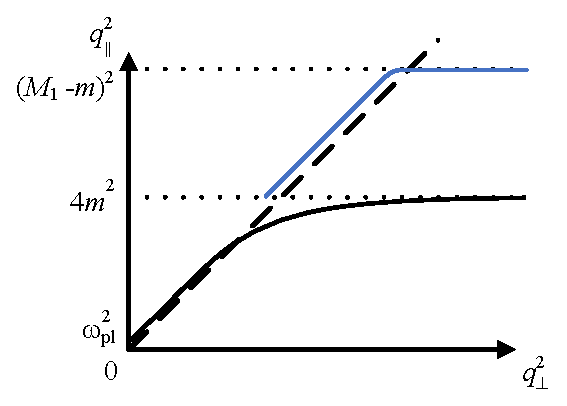
\includegraphics[scale=1.3]{DispFirst2ColOnly2Plasmas.eps}
	\caption{����� ��������� ���� 2 � �������� ������������ ������ ��� $B\gtrsim B_e$ ��������� ��������� �������. ��������� ������ ��������� ��������� ����� ���������, ������� ����������� ��������� � ������� ��������� ������ ���� 1. ������������� ������ ������� ���������� ������ ������� � �� ������� $q_{\mprl}^2>(M_1-m)^2$}.
	\label{fig:Disp}
\end{figure}

\textcolor{red}{��� ������ ���� 2 ������������� ������ � ������� ������ ������ ���������� �� ��������� �� ���������� �������, ������� ������������ �� ���������}:
	
\begin{equation}
	\omega_{p}^2 - {\cal P}^{(2)} (\omega_{p}, {\mathbf k} \to 0 ) = 0.
	\label{eq:omegapl}
\end{equation}

���������� ������� $\omega_{pl}$ ����� ����� ����������� ������ ������ � ������ �������������� �������, �.�. �������� ����� ������������ �������� ���������������� ��������� ������ ���� 2 �������� ������������� $\mathrm{Re} {\cal P}^{(2)}>0$, ��� ����� ��������� � ��������� ���������� ��������� � �������� ������. ��� ����������� � ������ $q_{\mprl}^2=4m^2$ ������������� ������ ����������� ����������� �� ���������� ������. � �������������� ������� ���� ������ $q_{\mprl}^2>4m^2$, ��� ����� �������� � ����� 2 ��������� �����������, ������������� ������ ������ ���� 2 ������ � ��������� ������ �� ���������� ������ $(M_1-m)^2$. ��� ������ ���� 1 ������������� ������ ����� ������� ���������, � $\omega_{pl}\simeq O(1/\beta)$.

������ ������ ������������ ������� ������������� ������ �� ��������� ������ �������� ��� ��������������. ��������, ����� ���� 2 ����� ���������� ����������� �� $e^+e^-$-���� ��� ��������� ������� $q^2_{\mprl}\gtrsim4m^2$. � ������ �������, ����� ���� 1 ����������� �� $e^+e^-$-���� � ������� $q^2_{\mprp}\gtrsim\left(M_1+m\right)^2$, ��� �������� ������ �������, � ������� ����������� ������ �������� �� ����������� ���������, \mbox{$q^2_{\mprl}\gtrsim\left(M_1-m\right)^2$}. ������� � ������� �������� ����\linebreak $B>20B_e$ ��� ������������ ������������ �������������� �������� ������������� ������������� ���� 2 ������ �������������� ���������: $\gamma^{(1)}e\to\gamma^{(1)}e$ �\linebreak $\gamma^{(1)}e\to\gamma^{(2)}e$. ����� ������� ��������, ��� ��������� ������� ������� ��������� � ������� ������������� ����������� �������� ���������������� ��������� (\ref{eq:Resonancew}). ��������������� ��������� ������ ����� ��� ������ ������������ ���������� ������� � ���������� ������������ ���������������� �����, ������� ��������������� �� ������ ����� ���� �����������. 
	
\section{������� ������������ �������������� ���������}\label{sec:Wcompton}

��� �������� �������������� �������� ������ ���������� ����� ������������ ����� $\delta$-����\-��\-��\-������� �����������, ������� ��� ������ � ������~\cite{Rumyantsev:2017}. ���������� � ������ ������ ���������� ������������ � ���� ������� � � ���������� ������������ � �����~\ref{sec:intro} ��������� ������������ ��� ������� ������ �������� ��������� � ������������� ������ ����������. ����� ����, ������ ������ ��������� ������~\cite{Rumyantsev:2017} ����� ��������� ������������� �������� � ��� ����������  � ���������� ������������.  ��� ������� ������ ���������� ������������ ���������� ������ ���������� ����������� ����������, ����������� �������� ����� �������������� �������� $f$ � ����������� ������~$j$~\cite{KuzRumShlen:2015}:
\begin{equation}
	{\cal L}(x) \, = \, \sum \limits_{k} g_k 
	[\bar {\psi_f}(x) \Gamma_k \psi_f(x)] J_k(x), 
	\label{eq:L}
\end{equation}
��� $\psi_f(x)$ --  
��������� ����������� ����, � ������ $k = S, P, V, A$ ������������� ���������, ���������������, ��������� � ���������� �������� � ��������� $\Gamma_k$:    
%\newline
$\Gamma_S = 1, \, \Gamma_P = \gamma_5, \, \Gamma_V = \gamma_{\alpha},
\, \Gamma_A = \gamma_{\alpha} \gamma_5$, ��������������� ���������� ���������� �����
$J_k(x)$ ($J_S$, $J_P$, $J_{V\alpha}$ ��� $J_{A\alpha}$), � ����� ���������� ��������������
$g_k$.

� ���������, ���������� ����������������� �������������� ����� ���� ����������� � ����:
%
\begin{eqnarray}\label{eq:L}
	{\cal L}(X) \, = \,- e [\bar \psi_f (X) \gamma^{\mu} A^{(\lambda)}_\mu (X) \psi_f(X)] \, ; 
	\label{eq:Lel}
\end{eqnarray}

\begin{figure}
	\centerline{
		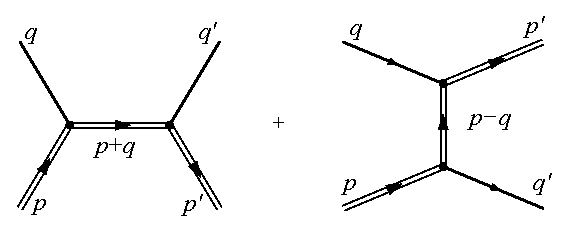
\includegraphics[width=10cm]{figComp1.eps}}
	\caption{��������� �������� ��� ������� $\gamma e \to \gamma^{\, \prime} e^{\, \prime}$. 
		������� ����� ��������, ��� ������� �������� ���� �� ��������� � �������� ��������� ��������� 
		� �� ���������� ����������  ������ �����.}
	\label{fig:Diagjj}
\end{figure}
%

������������� ������� � ��������� ����������� ����������� ����������� ��������, ��������������� �� ���.~\ref{fig:Diagjj}. ��������������� $S$-��������� ������� ��������� ������ ����������� $\lambda$ �� ��������� � ��������� ��������� � ������ ����������� $\lambda'$, � ������ �����������~(\ref{eq:L}) ����� ���� ����������� � ����:   
%
\beq                          
\nonumber
S^{s^{\, \prime} s}_{\gamma^{(\lambda)} e \to \gamma^{(\lambda')} e'} &=& - e^2\int \dd^4 X \dd^4 Y A^{(\lambda)}_\mu (X) A^{(\lambda')}_{\mu'} (Y)
%\times 
%\\[3mm]
%\nonumber
%&\times& 
\, \left [\bar \Psi^{s'}_{p',\ell'}(Y) \gamma_{\mu'} 
S(Y,X) 
\gamma_\mu \Psi^{s}_{p,\ell}(X) \right ]\, +
\\[3mm]
\label{eq:S1a}
&+& (A^{(\lambda)}_\mu, \gamma_\mu \leftrightarrow A^{(\lambda')}_{\mu'}, \gamma_{\mu'})\, .
\eeq

\noindent ����� $p^{\mu} = (E_{\ell}, {\bf p})$ � $p^{\, \prime \mu} =
(E^{\, \prime}_{\ell'}, {\bf p}^{\, \prime})$ - ������������� ������� 
�������-�������� ���������� � ��������� ���������, ����������� �� ������� ������ 
$\ell$ � $\ell'$  ��������������,
$\Psi^s_{p,\ell}(X)$ - �������� ������� ���������� � ����������� �������� 
���������� ����~(\ref{eq:psie}), $s$ � $s'$ ���������� 
��������������� ��������� ���������� � ��������� ��������� 
��������������, $S(Y,X)$ -- ���������� ��������� �� ������� ��������� ����~(��. ����������~\ref{appA:AccurProp}). 

�������� ������� ������ $A^{(\lambda)}_\mu(X)$ � $A^{(\lambda')}_{\mu'}(Y)$, � ���� �������,  ������ ����������� � ���� �������������� ������� � ����������� $\varepsilon^{(\lambda)}_\mu(q)$ � $\varepsilon^{(\lambda')}_{\mu'}(q')$:
%
\begin{eqnarray}
	\label{eq:j_k}
	A^{(\lambda)}_\mu (X) = \frac{e^{-\ii(qX)}}{\sqrt{2q_0 V}} \, \varepsilon^{(\lambda)}_\mu(q) \, , \quad  q^{\alpha} = (q_0, {\bs q})\, ,
\end{eqnarray}
%
\begin{eqnarray}
	\label{eq:j_k'}
	A^{(\lambda')}_{\mu'} (Y) = \frac{e^{\ii(q'Y)}}{\sqrt{2q'_0 V}} \, \varepsilon^{(\lambda')}_{\mu'}(q') \, , \quad  q'^{\alpha} = (q'_0, {\bs q'})\, , 
\end{eqnarray}
\noindent ���  $V = L_x L_y L_z$ -- ������������� �����.

� ������ ���� ���������, ��������� �������~(\ref{eq:psie}),  �����-������ �������� ������� �������~(\ref{eq:j_k}),
����������~(\ref{eq:propagator})  �~(\ref{eq:S1a}).  ��������������� ���������� ��������� �� $\dd X_0 \dd X_2 \dd X_3$ �  $\dd Y_0 \dd Y_2 \dd Y_3$,  ����������  $S$-��������� �������  � ��������� ����:
%
\begin{eqnarray}
	%\nonumber
	\label{eq:S2}                                  
	{\cal S}^{s^{\,\prime} s}_{\gamma^{(\lambda)} e\to \gamma^{(\lambda')} e} = \frac{\ii (2\pi)^3 
		\delta^{(3)}_{0,y,z} (P - p^{\, \prime} - q^{\, \prime})}
	{\sqrt{2q_0 V 2q^{\, \prime}_0 V 2 E_{\ell} L_y L_z 2 E^{\, \prime}_{\ell'}L_y L_z}}\, 
	{\cal M}^{s^{\, \prime} s}_{\gamma^{(\lambda)} e\to \gamma^{(\lambda')} e'} \, , 
\end{eqnarray}
\noindent ��� $\delta^{(3)}_{0,y,z} (P - p^{\, \prime} - q^{\, \prime}) 
= \delta (P_0 - E^{\, \prime}_{\ell'}-q^{\, \prime}_0) 
\delta (P_y - p^{\, \prime}_y - q^{\, \prime}_y) 
\delta (P_z - p^{\, \prime}_z - q^{\, \prime}_z)$, 


\begin{eqnarray}
	\label{eq:M12a}                                  
	%\nonumber
	&&{\cal M}^{s^{\, \prime} s}_{\gamma^{(\lambda)} e_\ell\to \gamma^{(\lambda')} e_{\ell'}} \simeq \ii e^2 \varepsilon^{(\lambda')}_{\, \mu'}(q') \varepsilon^{(\lambda)}_{\mu}(q) 
	%\times 
	%\\
	%\nonumber  
	%&&\times 
	\, \sum\limits_{n=0}^{\infty} \sum\limits_{s''} \; 
	\int \dd X_1 \dd Y_1 \eee^{-\ii X_1 q_x + \ii Y_1 q'_x}  \times
	\\ [3mm]
	\nonumber  
	&&\times \frac{\bar \phi^{s'}_{p', \ell'} (Y_1) \gamma_{\mu'} \phi^{s''}_{P, n} (Y_1) 
		\bar \phi^{s''}_{P, n} (X_1) \gamma_{\mu}  \phi^{s}_{p, \ell} (X_1)}
	{P^{2}_{\mprl} - M_n^2 + \ii P_0 \Gamma^{s''}_n/2} + 
	\\ [3mm]
	\nonumber  
	&&+ (\varepsilon^{(\lambda)}_\mu (q), \gamma_\mu, P, q \leftrightarrow \varepsilon^{(\lambda')}_{\mu'}(q'), \gamma_{\mu'}, P', -q')\, ,
\end{eqnarray}
\noindent  $P_\alpha = (p+q)_\alpha$, $P'_{\alpha} = (p-q')_{\alpha}, \,\, \alpha =0,2,3$.



�������, ��� ����� �������� ���������~(\ref{eq:M12a}) ����� ����� ����������� ��������. ���� ����������� ������� $\ell,\ell'\geqslant n$, �� � ���� ������ � ����������� �������� ���������� �����, ��������������� ����, ��� ����������� ������� ���������� ��������, �� ���� ����������� ��������� $P^{2}_{\mprl} - M_n^2 = 0$. ��� ������� $\ell,\ell'<n$ ������, ���������� �� ��������� � �����������, ����������� � �������� �� ����������� �������� �� �����������. ����� ����, �������������� ������ ����������, ��� ������ ������ ������������ ���������� �������� ����� � ��������� �������������� �������� $\gamma e\to \gamma e$ ����� ������ ������ ������ (�.�. s-���������) ���������.

\textcolor{red}{��������~\cite{Weldon:1983}, ������ ������ ��������� ��������� ��������� $\Gamma_n^{s''}$ ����� ����������� �
	���� ����� ����� ����������, $\Gamma^{(abs)\, s''}_n$, � ��������, $\Gamma^{(cr) \, s''}_n$,  ��������� 
	��������� �������:}
\beq
\label{eq:weldon}
\Gamma_n^{s''} = \Gamma^{(abs)\, s''}_n + \Gamma^{(cr) \, s''}_n \simeq 
\Gamma^{(abs) \, s''}_{e_n \to e_{\ell'} \gamma} 
\left [1+ \eee^{-(E^{\, \prime \prime}_n - \mu)/T} \right ]\, ,
\eeq
\noindent ���
%
\beq
\label{eq:e_abs}
\Gamma^{(abs) \, s''}_{e_n \to e_{\ell'} \gamma}  &=& \sum\limits_{\ell' = 0}^{n-1} \;  \sum\limits_{s' = \pm 1} \; \sum\limits_{\lambda'} \; 
\int \frac{\dd p'_y \dd p'_z  L_y L_z }{(2\pi)^2} \,[1 - f_{-}(E^{\, \prime}_{\ell'})] \times 
\\
\nonumber
&\times& \frac{\dd^3 q' V}{(2\pi)^3} \, (1 + f_{\omega'}) \;
\frac{|{\cal S}^{s^{\,\prime} s''}_{e_n \to e_{\ell'} \gamma^{(\lambda')}}|^2}{\tau}  
\eeq 
\noindent -- ������ ���������� ��������� � �������� $e_n \to e_{\ell'} \gamma$.

��� ���� �������� � ������~\cite{RumShlenYar:2017}, � ������, ����� ������ ���������� ��������� $\Gamma_n$ ���������� ����, �� ��������� �������������� �������� ������������� ����� �������������� ����������. ���� ���� ��� ����������� ����������� ��������� ���������� �������, ��� ��������, ��������, � ����������� ���������� �������������� ������� ��������� ��������. ������ ������ ���� ����� ����. �������������, � ������� ���������, ��� ����������� ������� $P_0\Gamma^{s''}_n\ll \left|P^2\mprl-M_n^2\right|$ ��������������� ����� �~(\ref{eq:M12a}) ����� ���� �������� $\delta$-��������:
\begin{equation}\nonumber
	\left|\frac{1}{P^2_{\mprl}-M_n^2-\ii P_0\Gamma^{s''}_n/2}\right|^2
	\simeq\frac{2\pi}{P_0\Gamma_n^{s''}} \delta(P^2_{\mprl}-M_n^2).
\end{equation}

� ����� ������ ������� ����������� ��������� ����� ��������� ��������� �������
\beq
\label{eq:delta_f}\nonumber
&&|{\cal M}^{s^{\, \prime} s}_{\gamma^{(\lambda)} e_\ell \to \gamma^{(\lambda')} e_{\ell'}}|^2 \simeq  \sum\limits_{s'' = \pm 1} \sum\limits_{n=0}^{\infty} \;  
\frac{\pi}{P_0 \; \Gamma_n^{s''}} \; \delta (P^{2}_{\mprl} - M_n^2) \times 
\\  
&&\times \left | 
\int \dd X_1 \dd Y_1 \bar \phi^{s'}_{p'\ell'} (Y_1) \phi^{s''}_{P, n} (Y_1) \bar \phi^{s''}_{P, n} (X_1) \phi^{s}_{p \ell} (X_1) \right |^2  \, .
\eeq

� ������~(\ref{eq:delta_f}) ������� $S$-���������� �������� �������� 
$jf \to j^{\, \prime} f^{\, \prime}$ ������������� ����� �������������� �������������
%
\beq
\label{eq:S2factor}
\nonumber 
&&\sum\limits_{s, s' = \pm 1} \frac{|{\cal S}^{s^{\,\prime} s}_{\gamma^{(\lambda)} e_\ell \to \gamma^{(\lambda')} e_{\ell'}}|^2}{\tau} = 
\sum\limits_{s, s', s'' = \pm 1} 
\sum\limits_{n=0}^{\infty} \; \frac{(2\pi)^3 \delta^{(3)}_{0,y,z} (P - p^{\, \prime} - q^{\, \prime})}
{2q_0 L_x 2q^{\, \prime}_0 V 2 E_{\ell} L_y L_z 2 E^{\, \prime}_{\ell'}L_y L_z} \times
\\[3mm] 
&&\times 
\int \frac{\dd p^{\, \prime \prime}_y \dd p^{\, \prime \prime}_z}{(2 E''_n)^2 (2 \pi)^2 \; \Gamma_n^{s''}} \, 
(2\pi)^3 \, \delta^{(3)}_{0,y,z} (P - p'') 
|{\cal M}^{s^{\, \prime} s''}_{e_n\to \gamma^{(\lambda')} e_{\ell'}}|^2 \; |{\cal M}^{s'' s}_{\gamma^{(\lambda)} e_\ell \to e_n}|^2   \, .
\eeq

����� �� ��������������� ��������� $\delta$ - �������:
%
\begin{eqnarray}
	\label{eq:delta_prop}
	\delta (P^2_{\mprl} - M^2_n) = \frac{1}{2 E''_n} \, \delta (P_0 - E''_n) \, , 
\end{eqnarray}
%
\noindent ��� $E''_n = \sqrt{p^{\, \prime \prime 2}_z + M^2_n}$. 


���� ������ ������   $S$-��������� ������� ���������� ��������� ��������� �������
\beq
%\nonumber
\label{eq:Sjf}                                  
{\cal S}^{s^{\,\prime \prime} s}_{\gamma^{(\lambda)} e_\ell \to e_n} = 
\frac{\ii (2\pi)^3 
	\delta^{(3)}_{0,y,z} (P - p^{\, \prime \prime})}
{\sqrt{2q_0 V 2 E_{\ell} L_y L_z 2 E^{''}_{n} L_y L_z}}\, 
{\cal M}^{s'' s}_{\gamma^{(\lambda)} e_\ell \to e_n} \, ,
\eeq
� ������ ����, ���
\begin{equation}
	\left|\delta^{(3)}_{0,y,z}(P-p'')\right|^2=\frac{1}{(2\pi)^2}\delta_{0,y,z}^{(3)}(P-p'')\tau L_y L_z \, ,
\end{equation}
�������� ������, ��� ���������~(\ref{eq:S2factor}) 
����� ����������� � �������������� ����:
%
\beq
\label{eq:S2factor1}
\sum\limits_{s, s' = \pm 1} \frac{|{\cal S}^{s^{\,\prime} s}_{{\gamma^{(\lambda)} e_\ell \to \gamma^{(\lambda')} e_{\ell'}}}|^2}{\tau} = 
\sum\limits_{s, s', s'' = \pm 1} 
\sum\limits_{n=0}^{\infty} \;  \int \frac{\dd p^{\, \prime \prime}_y 
	\dd p^{\, \prime \prime}_z}{(2 \pi)^2 \; \Gamma_n^{s''}} \,  
\frac{|{\cal S}^{s^{\,\prime \prime} s}_{\gamma^{(\lambda)} e_\ell \to e_n}|^2}{\tau} \, 
\frac{|{\cal S}^{s^{\,\prime} s''}_{ e_n \to \gamma^{(\lambda')} e_{\ell'}}|^2}{\tau} \, .
\eeq
\noindent ����� ��������������� ��������� ${\cal M}^{s'' s}_{\gamma^{(\lambda)} e_\ell \to e_n}$ �������������� �������� ������������ ��������� �������:
%
\beq
\label{eq:amplonever} 
{\cal M}^{s'' s}_{\gamma^{(\lambda)} e_\ell \to e_n} =  \frac{\exp{[-\ii q_x (p_y + p_y^{\,\prime \prime})/(2\beta)]}}{\sqrt{M_{\ell} M_n (M_{\ell} + m) 
		(M_n + m)}} 
\left [ \frac{q_y+\ii q_x}{\sqrt{q_{\mprp}^2}} \right ]^{n-\ell} {\cal T}^{s'' s}_{V} \, ,
\eeq

$S$-��������� ������� ��� �������� �������� ������ $\gamma \to e\gamma$ ����� ���� ������� �� ���������� �������� �������� ���������� ������ ��������� ������� 
$S_{e_n \to \gamma^{(\lambda')} e_{\ell'}}=S_{\gamma^{(\lambda)} e_\ell \to e_n}(q\to q', E_\ell \to E'_{\ell'})$.

����� �������, ��� ��������� ��������� �������������� �������� ������ ��������� � ������ ������ ����, ���������� ��������� ��������
${\cal T}^{s'' s}_{V}$, ������� ���� ������������ � ������~\cite{RumShlenYar:2017} � �������� � ����������~\ref{Sec:app_c} ��� ������ ����������, ����������������, ���������� � ���������-���������� �����. ��� ���������� ����� ���������
������-���������� � ����������~  � ���������������~$\{0, 3\}$:

\begin{equation}
	\label{eq:K1}
	{\cal K}_{1\alpha} = \sqrt{\frac{2}{(p\widetilde \Lambda p^{\, \prime \prime}) + 
			M_\ell M_{n}}} \left \{M_\ell (\widetilde \Lambda p^{\, \prime \prime})_\alpha + 
	M_{n} (\widetilde \Lambda p)_\alpha  \right \}\, ,
\end{equation}
%
\begin{equation}
	{\cal K}_{2\alpha} = \sqrt{\frac{2}{(p\widetilde \Lambda p^{\, \prime \prime}) + 
			M_\ell M_{n}}} \left \{M_\ell (\widetilde \varphi p^{\, \prime \prime})_\alpha + 
	M_{n} (\widetilde \varphi p)_\alpha  \right \}\, ,
	\label{eq:K2}
\end{equation}

\begin{equation}
	\label{eq:K3}
	{\cal K}_{3} = \sqrt{2\left [(p\widetilde \Lambda p^{\, \prime \prime}) + 
		M_\ell M_{n} \right]} \, ,  
\end{equation}
%
\begin{equation}
	\label{eq:K4}
	{\cal K}_4 = 
	- \sqrt{\frac{2}{(p\widetilde \Lambda p^{\, \prime \prime}) + M_\ell M_{n}}}\, 
	(p\widetilde \varphi p^{\, \prime \prime}) \, .
\end{equation}

��� ����������� ���� ������������ �����������:
%
\begin{equation}
	\label{eq:Ilnnl}
	\begin{aligned}
		\frac{1}{\sqrt{\pi}}\int \dd Z& \, \eee^{-Z^2}  
		H_n \!\! \left (Z + \frac{q_y + \ii q_x}{2\sqrt{\beta}} \right )   
		H_{\ell} \!\! \left (Z - \frac{q_y - \ii q_x}{2\sqrt{\beta}} \right ) =
		\\
		\nonumber
		&= 2^{(n+\ell)/2} \sqrt{n ! \, \ell !} 
		\left [\frac{q_y + \ii q_x}{\sqrt{q^2_{\mprp}}} \right ]^{n-\ell} 
		\eee^{{q^2_{\mprp}}/{(4\beta)}} 
		{\cal I}_{n, \ell} \!\! \left (\frac{q^{2}_{\mprp}}{2 \beta} \right ) \, , 
	\end{aligned}
\end{equation}
\noindent ��� ��� $n \geqslant \ell$
%
\begin{eqnarray}
	\nonumber
	&&{\cal I}_{n, \ell} (x) = \sqrt{\frac{\ell !}{n !}} \; \eee^{-x/2} x^{(n-\ell)/2} L_\ell^{n-\ell} (x) \, ,
	\\
	&&{\cal I}_{\ell, n} (x) = (-1)^{n-\ell} {\cal I}_{n, \ell} (x) \, ,
	\label{eq:Inl}
\end{eqnarray}
\noindent � $L^k_n (x)$ -- ���������� �������� �������~\cite{Gradshtein}.
� ���������� ������ ������������ ��������� ����������� ${\cal I}_{n, \ell}\equiv{\cal I}_{n, \ell} \left(\frac{q_\perp^2}{2\beta}\right)$, ${\cal I}_{n', \ell'}\equiv{\cal I}_{n', \ell'} \left(\frac{{q}_\perp^{\prime 2}}{2\beta}\right)$ � �.�. ��� �������������� ��������������� ���������, ��� ������� ���� ������ $\eta=-1$.

��� ��������������� ���������� ���������� ����������� ������ ������ ������� ������������ ����������� ���������� ������ -- ����������� �������� ������ � ������ ��������� �� ���� ��� ��� ���� ���������, ������� ��� �������������� �������� ��� ���������, ��������, � ������~\cite{Chistyakov:2009}:
\begin{eqnarray}\label{eq:WabsStrongB}
	&&W_{\gamma^{(\lambda)} e \to \gamma^{(\lambda')} e} = \frac{\beta}{16 (2\pi)^4
		\omega_{\lambda}}
	\int \mid {{\cal M}^{s'' s}_{\gamma^{(\lambda)} e_\ell \to \gamma^{(\lambda')} e_{\ell'}}}\mid^2 \times
	\label{eq:Wscatt}\\
	&&\times f_{E}\, [1-f_{E'}] \, (1 + f_{\omega'})
	\delta (\omega_{\lambda}({\bf k}) + E - \omega_{\lambda^{'}}({\bf k'}) - E')
	\frac{dp_z\,d^3 k^{'}}{ E E' \omega_{\lambda^{'}}},
	\nonumber
\end{eqnarray}
��� $f_{E}=(1+\exp[E/T])^{-1}$ -- ����������� ������� ������������� ���������� � ������������ $T$ � ������� ���������� �����������, \mbox{$f_\omega=(\exp[E/T]-1)^{-1}$} -- ����������� ������� ������������� �������. � ������� ������������ ���������� ������, ��������, ��������� ����� ���������� ������� \mbox{$\ell_\lambda=W^{-1}_{\gamma^{(\lambda)} e\to \gamma e}$}, � ���������������� ����������� ���������� ������ � ��������� ���������~(��. ����� 3).  

���������� ��������������� �������� ��������~(\ref{eq:delta_f}) � ������\linebreak (\ref{eq:S2factor})--(\ref{eq:amplonever}) � ���������~(\ref{eq:WabsStrongB}), �������� �� ��������������� ���������� ��������� ��������� � ������ � ������� ��������� ��������������, �������:

\beq
\label{eq:wabs1} 
&&W_{\gamma^{(1)} e \to \gamma e} = \frac{\alpha \beta}{2 \omega} 
\sum \limits^{\infty}_{\ell=0}  \sum \limits^{\infty}_{n=n_{0}} \sum \limits_{\epsilon = \pm 1} 
%\times 
%\\
%\nonumber
%&&\times 
\frac{f_{-}(E^{\epsilon}_{\ell}) [1 - f_{-}(E^{\epsilon}_{\ell} + \omega)]}{\sqrt{(M_n^2-M_{\ell}^2-q^{2}_{\mprl})^2-4 q^{2}_{\mprl}M_{\ell}^2}}
\times 
\\
\nonumber
&&\times 
\bigg \{ [2 \beta (n+\ell) - q^{2}_{\mprl}] ({\cal I}^2_{n,\ell-1}+{\cal I}^2_{n-1,\ell}) - 
%\\
%\nonumber
%&& -
8 \beta \sqrt{\ell n} {\cal I}_{n,\ell-1} {\cal I}_{n-1,\ell} \bigg \}   \, ,
\eeq
%

\beq
\label{eq:wabs2} 
&&W_{\gamma^{(2)} e \to \gamma e} = \frac{\alpha \beta}{2 \omega} 
\sum \limits^{\infty}_{\ell=0}  \sum \limits^{\infty}_{n=n_{0}} \sum \limits_{\epsilon = \pm 1} 
%\times 
%\\
%\nonumber
%&&\times 
\frac{f_{-}(E^{\epsilon}_{\ell}) [1 - f_{-}(E^{\epsilon}_{\ell} + \omega)]}{\sqrt{(M_n^2-M_{\ell}^2-q^{2}_{\mprl})^2-4 q^{2}_{\mprl}M_{\ell}^2}}
\times 
\\
\nonumber
&&\times 
\bigg \{ \left [\frac{(2\beta (n-\ell))^2}{q^{2}_{\mprl}} - 2 \beta (n+\ell) - 4 m^2 \right ] 
%\times 
%\\
%\nonumber
%&& \times 
({\cal I}^2_{n,\ell}+{\cal I}^2_{n-1,\ell-1}) -
\\
\nonumber
&&
-8 \beta \sqrt{\ell n} {\cal I}_{n,\ell} {\cal I}_{n-1,\ell-1} \bigg \}   \, ,
\eeq
���
\beq
\nonumber
&&E^{\epsilon}_{\ell} = \frac{1}{2 q^2_{\mprl}} \, \bigg [\omega \left (M^2_n - M^2_{\ell} - q^2_{\mprl} \right ) + 
\epsilon k_z 
\sqrt{\left (M^2_n - M^2_{\ell} - q^2_{\mprl} \right )^2 - 4 q^2_{\mprl} M^2_{\ell}} \, \bigg ] \, .
\eeq
\noindent �~(\ref{eq:wabs1}) �~(\ref{eq:wabs2}) 
������������ �� $n$ ���������� �������� ������ ���������� ������� � �������� ��������� �������:  
%
\beq
n_0 = \ell + \left [\frac{q^2_{\mprl} + 2 M_\ell \sqrt{q^2_{\mprl}}}{2 \beta} \right ] \, , 
\eeq
\noindent ��� $[x]$ -- ����� ����� ����� $x$.

� �������~\cite{Mushtukov:2016,Harding:1991,Schwarm:2017} ������������ ������� 
�������������� ��������� � ������������� ������ ��� ��������� ������������ � 
��������� �����, ����������� 
��� ����������� �������������� � ���������� $10^{12}-10^{15}$ ��. � ������ 
������� ���������� ������� ��������� ��� �������, ��� ��������� � �������� 
��������� ��������� �� �������� ������ ������. ��� �������� ���������� �������� 
�� ����������� ��������� � �������� �������, ���������� � �������������� 
���������� ������� ��������� ������~(\ref{eq:psie}).
\newpage

� ������ ������� ������� ������������� �� ��������� ���������� 
��������� � ������� ����� ������
� ������������� �������� ������������� $\overline{f}_{n,s}(p_z)$:
\begin{equation}\label{eq:dsigma}
	\sigma^*_\lambda=\int_{-\infty}^{\infty} 
	\overline{f}_{n,s}(p_z)\dd\sigma_{\gamma^{(\lambda)} e\to \gamma e}\, ,
\end{equation}
��� 
\begin{equation}
	d\sigma_{\gamma^{(\lambda)} e\to \gamma e}= \frac{dW_{\gamma^{(\lambda)} e \to \gamma e}}{j},
\end{equation}
$j=|(pq)_{\mprl}|/(E \omega V)$ -- ��������� ������ �������� 
������  � ���������� �� ��������� � ���������� ���� ���������������. ������ �� 
���������� ������� �������������:
\begin{equation}
	\sum_{n,s}\int_{-\infty}^{\infty} \dd p_z \overline{f}_{n,s}(p_z)=1,
\end{equation}
���������� � � ����:
\begin{equation}
	\overline{f}_{n,s}(p_z)=\frac{\beta}{(2\pi)^2n_e}\frac{1}{e^{E_n/T}+1},
\end{equation}
��� 
\begin{equation}\label{eq:ne}
	n_e = \frac{\beta}{(2 \pi)^2} \sum \limits^{\infty}_{\ell=0} 
	(2-\delta_{\ell,0}) \int \limits^{\infty}_{-\infty}\dd p_z f_{-}(E_{\ell})
\end{equation}
-- ������������ ���������� �� ������� ��������� ����.

� ������ (\ref{eq:dsigma}) -- (\ref{eq:ne}) ���������������� ������� ���������, ���������������� �� 
������������ ��������� ������, ����� ���� �������� ����� ���������������� 
����������� ����������:
\begin{equation}
	d\sigma^*_\lambda=\frac{E\omega}{(pq)_{\mprl}}\frac{1}{n_e} 
	dW_{\gamma^{(\lambda)} e\to\gamma e}\, .
\end{equation}

������� ��������, ��� ��� ����������������� ������������ ����������, ������ 
���������������� �� ��������� 
���������� 
���������, � 
���������������� ������� ��������� � ��������� ������������ �����������~\cite{Landau:1989}:
\begin{equation}
W_{\gamma^{(\lambda)} e\to\gamma e}=\frac{1}{\ell_\lambda}=n_e 
\sigma_{\gamma^{(\lambda)} e\to\gamma e}\, .
\end{equation}

�������� �������~\ref{fig:Disp} �������~\ref{Ch:Propagator} ��� ��������������� ���������� ���������� ���� � ������, ����� �������, ��� ����� ��������� ��� ���� 1, ��� � ���� 2, � ������������� $\omega_{pl}$, ���� ���������� �� ���������� �� ����������� ����� ����������. � ����� ������ ������������ ���������� ���� ���������� �������� ������ ����� ��������
$q_z \simeq \omega \sin{\theta}$, ��� 
$\theta$ -- ���� ����� ��������� ������ � ������������ ���������� ����. ��� ��� ���������� � �������~\ref{Ch:Propagator}, �������������� �������� ������� ������� ���������� ������������ ������ ������������ ���������� $q^2_{\mprl} \simeq (M_n+M_{\ell})^2$, ������, ��� ���������� ������, ��� �������� ���������� ���� $B\simeq 10^{12}$ �� ��� ���������� �������������� ���, ���~$Z_{1,2}\simeq 1$. 

������������� ������ ������������ ������� �� ������������ ��������� ������ $\sigma^*/\sigma_T$  � ������������ ������~\cite{Harding:1991} ��� ��������� �������� ���������� ���� (\mbox{$B=0.039B_e\simeq1.7\times10^{12}$ �� � $B=0.23B_e=10^{13}$ ��}) � ���������� ($T=5$ ��� � $T=50$ ���) ����������� ��~���. \ref{fig:Harding1}--\ref{fig:Harding4}. ���������� ���������� ����������, ��� ������-�������������� ����������� ���������� ������ ��������� ����������� ����. � ������� ��������� ������� �������������� ��������� �������� ��������� ������� � ������ �������� ������, ��� ��� ����������� ����������� ��������� �� ���� ����������� ������� ��� ������-�������������� ����������� ������ ���� ������������ ����� � ��������. � ����������� ����������� (���.~\ref{fig:Harding2} �~\ref{fig:Harding4}), ������ �������� ����������� �����, ����� ����������� ���������� �������� ������-��������������� ����������� �������� ��� ����� ����� ����� ������������ ��������������� ������ � ���������� ����. ��� ���������� ���������� ���� (���.~\ref{fig:Harding3}--\ref{fig:Harding4}) ����������� �������� ����������� �����, �������� �������~\ref{eq:whn}, � ����� �� ������� ��� ���������� �����. 

������������ ������� ����������� ������� ��������� � ������ ����, ��� �������� �������� ����� �������� ������������ ������� ������. ��� ����������� $T=5$ ��� ����� �������� ������������, ��� ��������� ��������� �������� �������� ������� ������, ��� ��� ��� ����������� �� ������ ����� � ������� ���������. � ������ �������, ��� ����������� $T=50$ ���, ��� �������� �� ��������~\ref{fig:HardingManyLevels}, ������� � ������� ��������� ������������� � ������ ���������� ���� ����������. ����� � ������� ������������ ����� ���������, ��������� � ���������� (��., ��������,~\cite{Pavlov:1991,Klepikov:1954,Baier:2007}), ��������������� �������� $\omega_{n\ell}=(M_n-M_\ell)/\sin \theta$, ������� �������� ���� ����������� ��� �������, ������������������ ������� ���������� ����, �� ������ ����� ����� � ������������ ��������.

��������� �������� ������� � ������ �������� ������, ������� ���� ����� �������� �� ����������� ������~\cite{Mushtukov:2016}, ����� ���������� �������� �� ���� ������� ������� ������� (��. ���.~\ref{fig:CompAndMushXGround}--\ref{fig:CompAndMushO}). ��������� ���������, ���������� � ���� ������, ������� �������������� ��������� ���� ��������� �~\cite{Schwarm:2017}, ��� ���� ���������� ��������� ���������� �~\cite{Schwarm:2017}  ��������� � ������������, ��������������� � ��������� �����������. ��� ����� ���� ������� � ���������� ������������ ��� ���������� �������� � ������~\cite{Mushtukov:2016}. \textcolor{red}{� ������� �� ������� ������ ������������ ��������.}


����� �������, ���������� 
�����������~(\ref{eq:delta_f}) ����������  � ������� ����� $B \sim 10^{12}-10^{15}$ ��, ����������� ��� ���������� � ��������������. � ������ �������, ���������� ������������ ���������� ������~(\ref{eq:wabs1}) �~(\ref{eq:wabs2}) ������������ ������ ��� ����� �������� ��������� (�� ����������� ��������� �����, ��������� �����), ��� �������� ������� ����� ������� � ����������� (��������, � ������� ������ �������� ���������), ��� ������ ���� �������� ������.

\begin{figure}[t!]
	\centering
	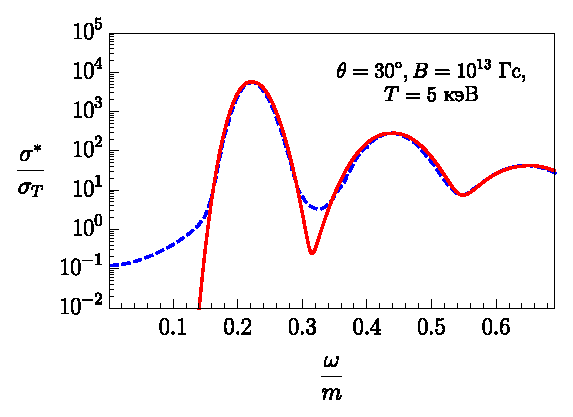
\includegraphics[width=0.6\linewidth,clip]{AliceDeltaAverageB023T001Deg30.eps}
	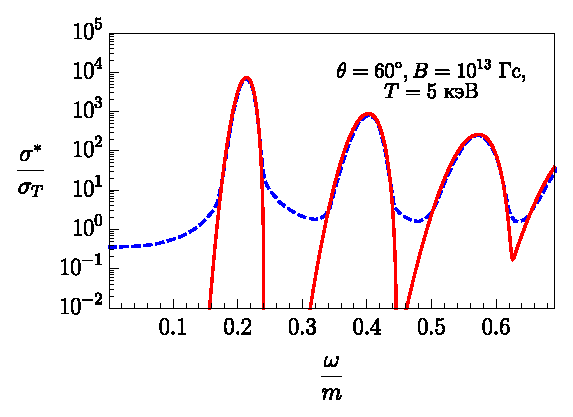
\includegraphics[width=0.6\linewidth,clip]{AliceDeltaAverageB023T001Deg60.eps}
	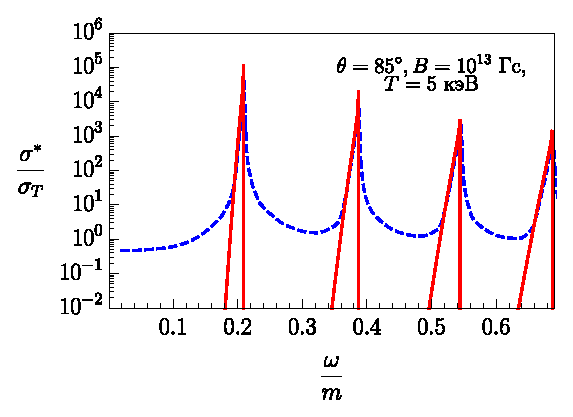
\includegraphics[width=0.6\linewidth,clip]{AliceDeltaAverageB023T001Deg85.eps}
	\caption{C������ (� �������� $\sigma_T$), ������������ �� ������������ ���������� ������, $e\gamma^{(2)}  \to e\gamma$, ���������� � ������~\cite{Harding:1991} (���������� �����) � $\delta$-�������������� ����������� (�������� �����) ��� ��������� ����� $\theta$ ����� ��������� ������ � ������������ ���������� ����. ��� ��������� � �������� ��������� ��������� �� �������� ������ ������. �������� ����������� $T=5$ ���, � ���������� ���� -- $B=10^{13}$ ��.\label{fig:Harding1}}
\end{figure}

\begin{figure}[t!]\centering
	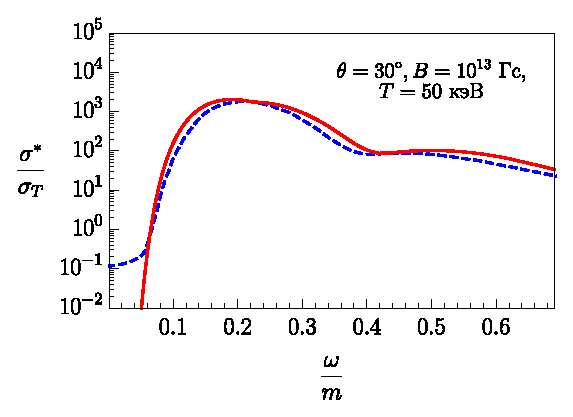
\includegraphics[width=0.6\linewidth,clip]{AliceDeltaAverageB023T01Deg30.eps}
	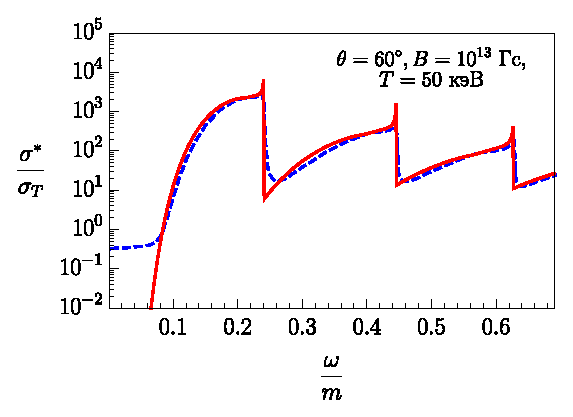
\includegraphics[width=0.6\linewidth,clip]{AliceDeltaAverageB023T01Deg60.eps}
	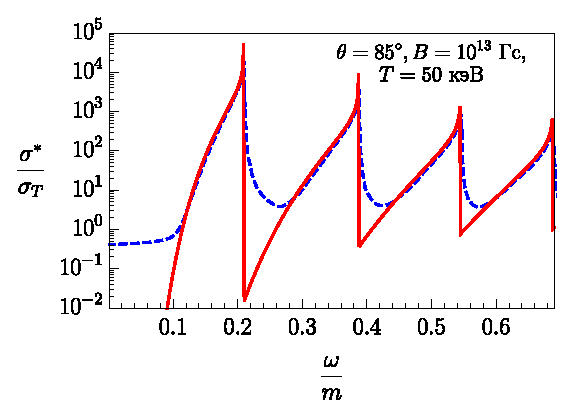
\includegraphics[width=0.6\linewidth,clip]{AliceDeltaAverageB023T01Deg85.eps}
	\caption{�� ��, ��� � �� ���.~\ref{fig:Harding1} ��� ����������� $T=50 ���$ � ���������� ���� $B=10^{13}$~��.\label{fig:Harding2}}
\end{figure}

\begin{figure}[t!]\centering
	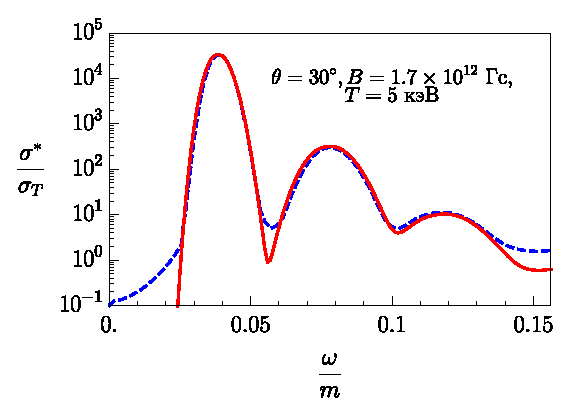
\includegraphics[width=0.6\linewidth,clip]{AliceDeltaAverageB0039T001Deg30.eps}
	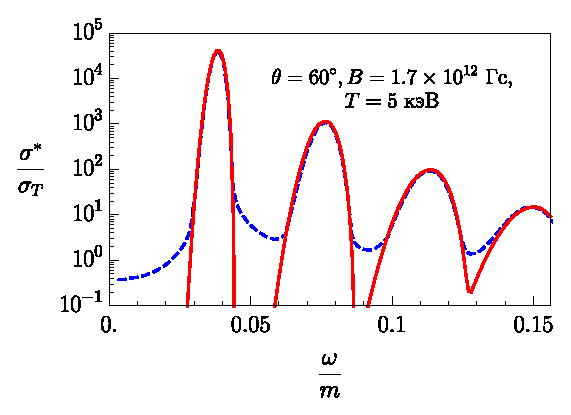
\includegraphics[width=0.6\linewidth,clip]{AliceDeltaAverageB0039T001Deg60.eps}
	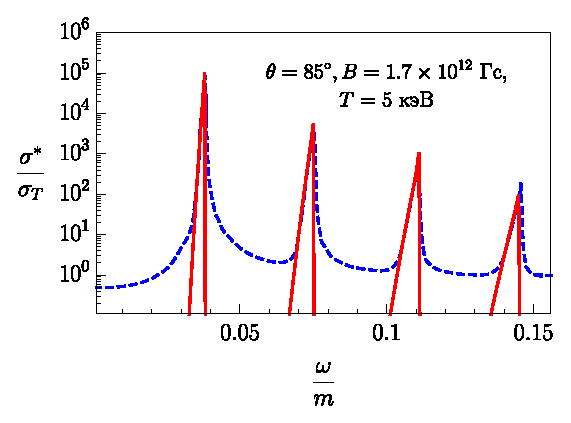
\includegraphics[width=0.6\linewidth,clip]{AliceDeltaAverageB0039T001Deg85.eps}
	\caption{�� ��, ��� � �� ���.~\ref{fig:Harding1} ��� ����������� $T=5 ���$ � ���������� ���� $B=1.7\times 10^{12}$~��.\label{fig:Harding3}}		
\end{figure}

\begin{figure}[t!]\centering
	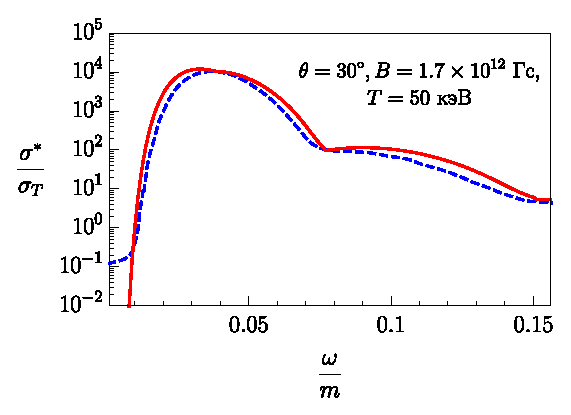
\includegraphics[width=0.6\linewidth,clip]{AliceDeltaAverageB0039T01Deg30.eps}
	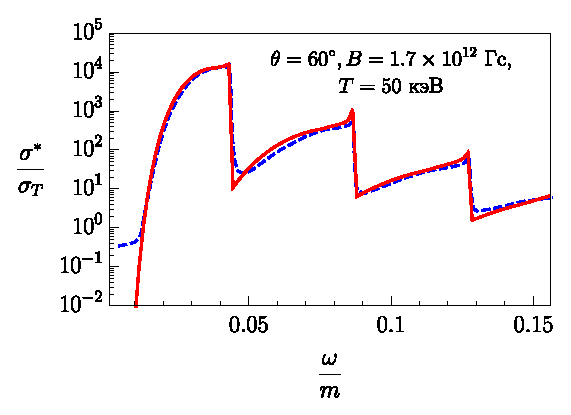
\includegraphics[width=0.6\linewidth,clip]{AliceDeltaAverageB0039T01Deg60.eps}
	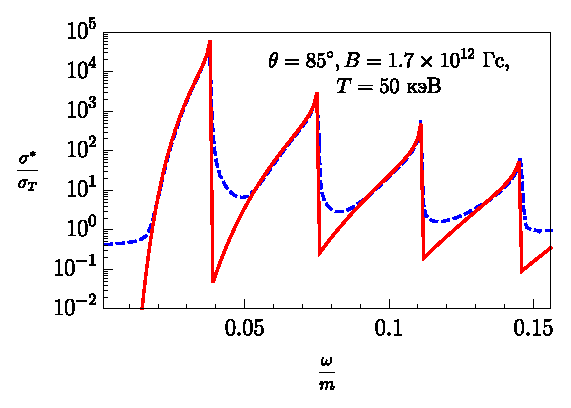
\includegraphics[width=0.6\linewidth,clip]{AliceDeltaAverageB0039T01Deg85.eps}
	\caption{�� ��, ��� � �� ���.~\ref{fig:Harding1} ��� ����������� $T=50 ���$ � ���������� ���� $B=1.7\times 10^{12}$~��.\label{fig:Harding4}}
\end{figure}
\clearpage
\begin{figure}[t!]\centering
	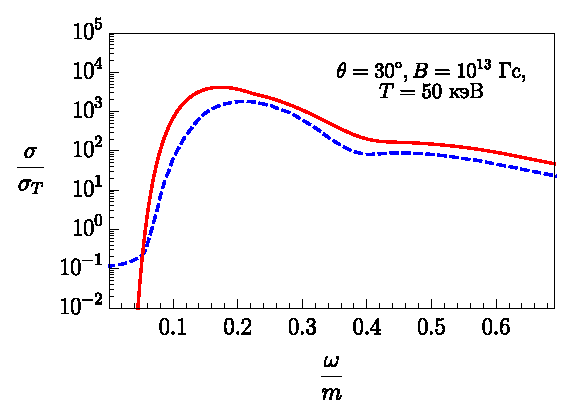
\includegraphics[width=0.6\linewidth,clip]{AliceDeltaManyLevelB023T01Deg30.eps}
	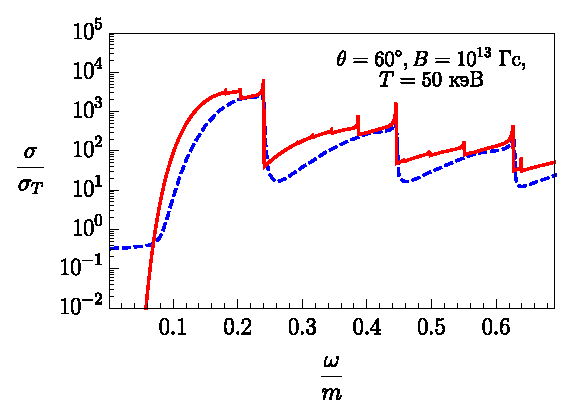
\includegraphics[width=0.6\linewidth,clip]{AliceDeltaManyLevelB023T01Deg60.eps}
	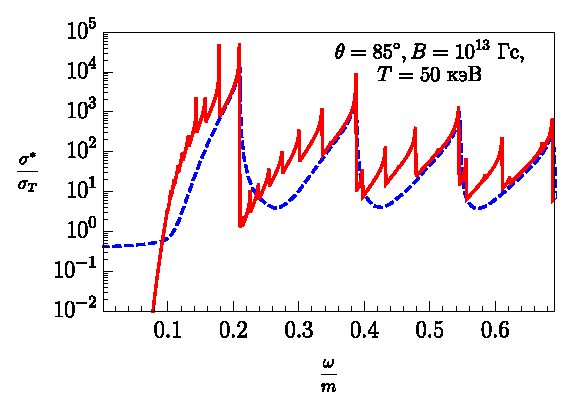
\includegraphics[width=0.6\linewidth,clip]{AliceDeltaManyLevelB023T01Deg85.eps}
	\caption{C������ (� �������� $\sigma_T$), ������������ �� ������������ ���������� ������ � �� ������������ ���������� ���������, $e\gamma^{(2)}  \to e\gamma$, ���������� � ������~\cite{Harding:1991} (���������� �����) � $\delta$-�������������� ����������� (�������� �����) ��� ��������� ����� $\theta$ ����� ��������� ������ � ������������ ���������� ����. �� ��������� ���������� ���. �������� ����������� $T=50$ ���, � ���������� ���� -- $B=10^{13}$ ��.\label{fig:HardingManyLevels}}
\end{figure}



\begin{figure}[t]\centering
	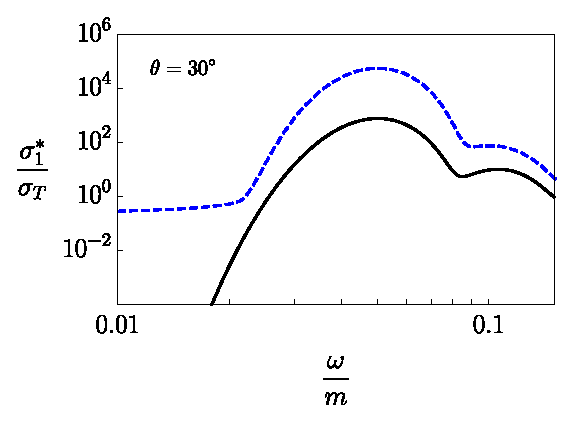
\includegraphics[width=0.6\linewidth,clip]{CompareMushOs005MushtukovX1Ground.eps}
	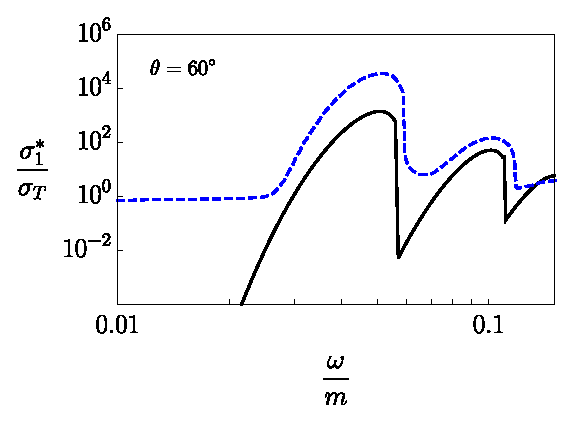
\includegraphics[width=0.6\linewidth,clip]{CompareMushOs005MushtukovX2Ground.eps}
	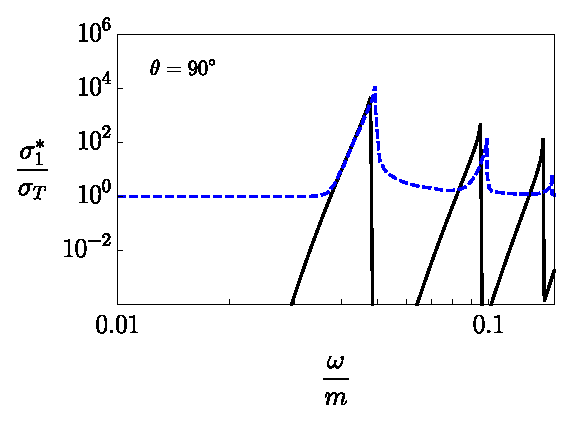
\includegraphics[width=0.6\linewidth,clip]{CompareMushOs005MushtukovX3Ground.eps}
	\caption{C������ (� �������� $\sigma_T$) ��������� ������ ���� 1, $e\gamma^{(1)}  \to e\gamma$, ���������� � ������~\cite{Mushtukov:2016} (���������� �����) � $\delta$-�������������� ����������� (�������� �����) ��� ��������� ����� $\theta$ ����� ��������� ���������� ������ � ������������ ���������� ���� (�������� ���������� �� ��������). $B=2.2\times 10^{12}$ ��, $T = 20$ ���, $\mu=0$. ��������� � �������� ��������� ��������� �� �������� ������ ������.	\label{fig:CompAndMushXGround}}

\end{figure}
\begin{figure}[t!]\centering
	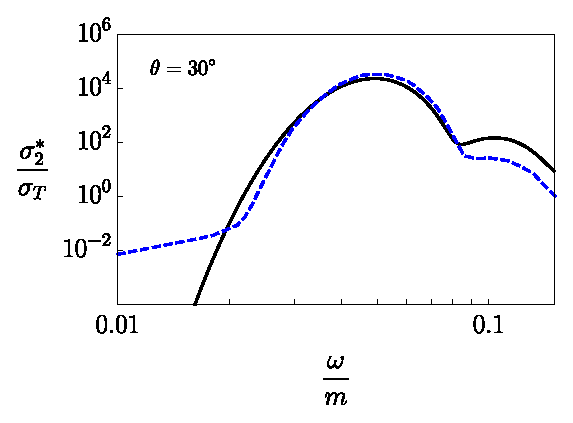
\includegraphics[width=0.6\linewidth,clip]{CompareMushOs005MushtukovO1Ground.eps}
	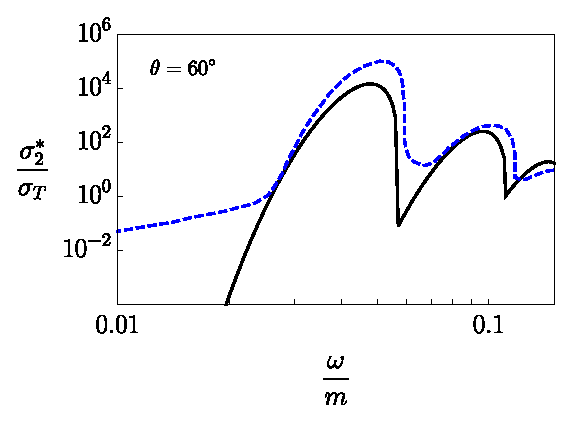
\includegraphics[width=0.6\linewidth,clip]{CompareMushOs005MushtukovO2Ground.eps}
	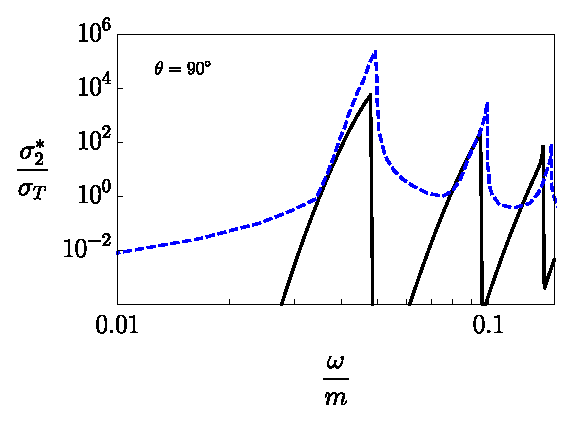
\includegraphics[width=0.6\linewidth,clip]{CompareMushOs005MushtukovO3Ground.eps}
	\caption{�� ��, ��� � �� ���.~\ref{fig:CompAndMushXGround} ��� ���������� ������ $B=2.2\times 10^{12}$ ��, $T = 20$ ���, $\mu=0$.	\label{fig:CompAndMushO}}
\end{figure}
\clearpage

\section{������� �������������� ��������� � ������������ ������� ��������� ���� � ������ ������ ������������ ����}

���������� ������ �������� ������������� ���������� ����, \linebreak\mbox{$B\sim 10^{15}-10^{16}$} �� � ������� ���������� $T=1$ ���, ������� ���������� ��� ���������� ������� SGR (���������� ������ ������������� �����-���������).  ������������ �������������� �������� � ��������� ����� ���������� �������� ���� ���������, ��������, � ������~\cite{Chistyakov:2009}. ������, ���������� � ���� ������������ ���������� ����� ������������� ������ ��� ������� ������� ������� ����� �� ����������. ������� ������������ ��������������� ������� ��������� ����������� ���������� ������ � ������� �������� ���� � ������ ���������� ��������� �� ����������� ��������� � �������� ������� ������������ ���� � �������� � ������������� ��������~\cite{Chistyakov:2009} � ������-�������������� ������������~\cite{RumShlenYar:2017}. \textcolor{red}{��������� � ������� �������� ���������� ���� ��������� � �������� ��������� ����� ��������������� �������� �������� ������� ������, � ����������� �������� -- ������ ������� ������, �� ����������� ���������� ������ � ������ �������� ������ ������������ ���� ������ ���������� ������� ��� ���������� ���}. ��� ���� �������� � ������� 1.3, � ������� ��������� ���� ������� ������, �� ������� ����������� ��������, ����, ��� ����� �������� $e^+e^-$ ���� $q_{\mprl}^2=4m^2$ ��� ������ ���� 2 , �� ������������� ����������� ������ ������ ��������� $e\gamma^{(1)}\to e\gamma^{(1)}$ � $e\gamma^{(1)}\to e\gamma^{(2)}$. ������� ��������, ��� ��� ������ ����~1 ����� �������� $e^+e^-$ ���� $q_{\mprl}^2=(M_1+m)^2$ �������� ���� ��������������� ������� ��������� $q_{\mprl}^2=(M_1-m)^2$.

������ �� ����������� ������~\cite{Chistyakov:2009}, ���������� ����������� ��������� �������������� �������� � ������� �������� ���������� ���� � ����:
\begin{equation}\begin{gathered}\label{amplnonres}
		{\cal M}_{e\gamma^{(1)}\to e\gamma^{(1)}}=\frac{8i\pi\alpha m}{\beta}\frac{(q\varphi q')(q\tilde{\varphi}q')}{\sqrt{q^2_\perp q^{'2}_\perp (-Q^2_{\mprl})}}\, ,\\
		{\cal M}_{e\gamma^{(1)}\to e\gamma^{(2)}}=\frac{8i \pi\alpha m}{\beta}\frac{(q\Lambda q')(q\tilde{\Lambda} Q)}{\sqrt{q^2_\perp {q'}^2_{\mprl}(-Q^2_{\mprl})}}\, ,\hspace{2mm} 
\end{gathered}\end{equation}
���   
$Q^2_{\mprl} = (q - q')^2_{\mprl} <0$,
$q_{\alpha} = (\omega,{\bf k})$ � $q'_{\alpha} = (\omega',{\bf k'})$
-- 4-�������� ���������� � ��������� ������� ��������������.

����� ����������� (\ref{amplnonres}) �
(\ref{eq:WabsStrongB}) ������������ ���������� ������ ��� ������� $e\gamma^{(1)}\to e\gamma^{(1)}$ � $e\gamma^{(1)}\to e\gamma^{(2)}$ � ������������� ������� ��� �������, ������������������ ��� ����� $\theta=90^\circ$ �� ��������� � ����������� ���������� ����,  ����� ���� ������������ ��������� �������:
\begin{equation}\label{Wnonres}\begin{aligned}
		W_{e\gamma^{(1)}\to e\gamma^{(1)}}&=\frac{\omega \alpha^2m^2}{2 \beta \pi}\int dQ_0 dk_z' \frac{{k_z'}^2}{(-Q_{\mprl}^2)^2\varkappa}\theta(-Q_{\mprl}l^2)
		\theta({q'}_{\mprl}^2)\times\\&\times \sum_{\sigma} f(E_\sigma)(1-f(E_\sigma+\omega))(1+f_{\omega'})\, ,
\end{aligned}\end{equation}
\begin{equation}
	\begin{aligned}\label{Wnonres2}
		W_{e\gamma^{(1)}\to e\gamma^{(2)}}&=\frac{ \alpha^2m^2}{2 \beta \pi \omega}\int dQ_0 dk_z'\left(1-\frac{{\cal P}^{(2)}(q')}{{q'}_{\mprl}^2}\right) \frac{{q'}_{\mprl}^2-\omega\omega'}{(-Q_{\mprl}^2)^2\varkappa}\theta(-Q_{\mprl}^2)
		\theta({q'}_{\mprl}^2)\times\\ &\times\sum_{\sigma} f_{E_\sigma}(1-f_{E_\sigma+\omega})(1+f_{\omega'})\, ,
	\end{aligned}
\end{equation}
\noindent ��� $\theta(x)$ -- ������� ���������,
\mbox{$\varkappa = \sqrt{1 - 4m^2/Q^2_{\mprl}}$, $E_\sigma=\sqrt{p_{z\sigma}^2+m^2}$}, � \linebreak $p_{z\sigma}$ -- ����� ��������� $Q_0+E_\sigma-E'_\sigma=0$:
\begin{equation}\label{savelaw}
	p_{z\sigma}=-\frac{Q_z}{2}+ \sigma Q_0 \varkappa\, .
\end{equation} 

���������������� ������������ ������~\cite{Chistyakov:2009}, ��������� ${\cal M}_{e\gamma^{(1)}\to e\gamma^{(1)}}$, ${\cal M}_{e\gamma^{(1)}\to e\gamma^{(2)}}$ � ������� �������� ���������� ���� � � ������ �������� ������ ������������ ���� ����� ����������� ��������� �������:
\begin{equation}\label{Mres}
	\begin{aligned}
		{\cal M}_{e\gamma^{(1)}\to e\gamma^{(1)}}=& \frac{8m\pi\alpha}{\sqrt{(-Q^2_{\mprl})}} \exp\left[-\frac{q^2_\perp+q'^2_\perp-2i(q\varphi q')}{4\beta}\right]\cdot\frac{1}{\sqrt{q^2_\perp q'^2_\perp}}\times 
		\\ &\times \sum_{n=1}^{\infty}\frac{((q\Lambda
			q')-i(q\varphi
			q'))^{n}}{(n-1)!(2\beta)^{n-1}}
		\frac{(q\tilde{\varphi}q')}{(p+q)^2_{\mprl}-M_n^2+iE''_n\Gamma_n }+\\
		&+(q\leftrightarrow-q')\, ,
	\end{aligned}
\end{equation}
\begin{equation}\label{Mres12}
	\begin{aligned}
		{\cal M}_{e\gamma^{(1)}\to e\gamma^{(2)}}=& \frac{8m\pi\alpha}{\sqrt{(-Q^2_{\mprl})}} \exp\left[-\frac{q^2_\perp+q'^2_\perp-2i(q\varphi q')}{4\beta}\right]\cdot\frac{1}{\sqrt{q^2_\perp q'^2_{\mprl}}}\times 
		\\ &\times \sum_{n=1}^{\infty}\frac{((q\Lambda
			q')-i(q\varphi
			q'))^{n}}{(n-1)!(2\beta)^{n-1}}
		\frac{(Q\tilde{\Lambda}q')}{(p+q)^2_{\mprl}-M_n^2+iE''_n\Gamma_n }+\\
		&+(q\leftrightarrow-q')\, ,
	\end{aligned}
\end{equation}
��� ������ ������ ���������� ��������� $\Gamma_n$  �������� ����������~(\ref{eq:weldon}). \linebreak � ������ �������, ��� ���������� ��������� ������, � ������ ������ �������������, �������, ��������-������������ ������ ������ ������ ���������� ��������� ���� ���������� �� ���������������� ��������� � ������� ��������� ���� � �������������������� ����������~\cite{KM_Book_2013}:
\begin{equation}\label{Shir}
	\begin{aligned}
		E''_n\Gamma_n=&\alpha \beta \sum_{n'=0}^{n-1}\int_{0}^{(\sqrt{n}-\sqrt{n'})^2}\frac{dx}{\sqrt{(n+n'-x)^2-4n n'}}\times\\
		&\times\{(n+n'-x)[{\cal I}^2_{n,n'-1}(x)+{\cal I}^2_{n-1,n'}(x)]-\\
		&-4\sqrt{nn'}{\cal I}_{n,n'}(x){\cal I}_{n-1,n'-1}(x)\}\, ,
	\end{aligned}
\end{equation}
��� $E''_n=E+\omega$ -- ������� ������������ ���������.

 ����������� ������������ ���������� ������ ��� �������\linebreak $e \gamma^{(1)} \to e\gamma^{(1)}$ � $e \gamma^{(1)} \to e\gamma^{(2)}$ � ������ �������� ������ ���������� ��������� ����� ���� �������� ������������ ��������~(\ref{Mres}) �~(\ref{Mres12}) �~(\ref{eq:WabsStrongB}) � � ������, ����� ��������� ����� ���������������� ������� ���������� ����, ������������ ���������� ����� ����������� ��������� �������:

\begin{equation}
	\begin{aligned}\label{Wres}
		&W_{e\gamma^{(1)}\to e\gamma^{(1)}}=\frac{\beta\alpha^2m^2}{\pi} \int dQ_0dk'_z \frac{{k_z'}^2\omega } {(-Q_{\mprl}^2)^2\varkappa}\exp\left[-\frac{\omega^2+{q'}_\perp^2}{2\beta}\right]\times\\ 
		&\times\sum_{n=1}^{\infty}\sum_{\sigma=\pm 1}\frac{1}{[(n-1)!]^2}\left(\frac{\omega \sqrt{q_\perp'^2}}{2\beta}\right)^{2(n-1)}\bigg\{
		\frac{1}{((p_\sigma+q)_{\mprl}^2-M_n^2)^2+(E''_n\Gamma_n)^2}  +\\
		&+\frac{1}{((p_\sigma-q')_{\mprl}^2-M_n^2)^2+(E''_n\Gamma_n)^2}-
		\\
		&-2
		\sum_{n'=1}^{\infty}\frac{(n-1)!}{(n'-1)!}\left(\frac{\omega \sqrt{q_\perp'^2}}{2\beta}\right)^{n'-n}J_{n+n'}\left(\frac{\omega \sqrt{q_\perp'^2}}{\beta}\right)\times\\
		&\times\frac{[(p_\sigma+q)^2_{\mprl}-M_n^2][(p_\sigma-q')^2_{\mprl}-M^2_{n'}]+E''_n\Gamma_nE''_{n'}\Gamma_{n'}}{[((p_\sigma-q')_{\mprl}^2-M_n^2)^2+(E''_n\Gamma_n)^2][((p_\sigma+q)_{\mprl}^2-M_{n'}^2)^2+(E''_n\Gamma_{n'})^2]}
		\bigg\}\times
		\\&\times f_{E_\sigma}(1-f_{E_\sigma+Q_0})(1+f_{\omega'}
		) \, ,
	\end{aligned}
\end{equation}

\begin{equation}
	\begin{aligned}\label{Wres2}
		&W_{e\gamma^{(1)}\to e\gamma^{(2)}}=\frac{\beta\alpha^2m^2}{\pi} \int dQ_0dk'_z \frac{q_\perp'^2\omega } {(-Q_{\mprl}^2)^2\varkappa}\exp\left[-\frac{q_\perp^2+{q'}_\perp^2}{2\beta}\right]\times\\ 
		&\times\sum_{n=1}^{\infty}\sum_{\sigma=\pm 1}\frac{1}{[(n-1)!]^2}\left(\frac{\omega \sqrt{q_\perp'^2}}{2\beta}\right)^{2(n-1)}\bigg\{
		\frac{Q_0/\omega}{((p_\sigma+q)_{\mprl}^2-M_n^2)^2+(E''_n\Gamma_n)^2}+
		\\
		&+\frac{Q_0^2/q'^2_{\mprl}}{((p_\sigma-q')_{\mprl}^2-M_n^2)^2+(E''_n\Gamma_n)^2}-
		\\
		&-2
		\sum_{n'=1}^{\infty}\frac{(n-1)!}{(n'-1)!}\left(\frac{\omega \sqrt{q_\perp'^2}}{2\beta}\right)^{n'-n} J_{n+n'}\left(\frac{\omega \sqrt{q_\perp'^2}}{\beta}\right)\times\\
		&\times\frac{[(p_\sigma+q)^2_{\mprl}-M_n^2][(p_\sigma-q')^2_{\mprl}-M^2_{n'}]+E''_n\Gamma_nE''_{n'}\Gamma_{n'}}{[((p_\sigma-q')_{\mprl}^2-M_n^2)^2+(E''_n\Gamma_n)^2][((p_\sigma+q)_{\mprl}^2-M_{n'}^2)^2+(E''_n\Gamma_{n'})^2]}
		\times\\&\times
		\frac{Q_0^2(\omega-Q_0)}{\omega q'^2_\perp}
		\bigg\}\times f_{E_\sigma}(1-f_{E_\sigma+Q_0})(1+f_{\omega'}
		) \, ,
	\end{aligned}
\end{equation}
\noindent ��� $J_n(x)$ -- ������� ������� ������ �������, $p^\alpha_{\sigma\mprl}=(E_\sigma,p_{z\sigma})$. ���������� ������������ �������� ��������� ������ ������������ �� ��������� ���������:
\begin{equation}
	q'^2_{\mprl}=q'^{2}_\perp + {\cal P}^{(\lambda)}(q') .
\end{equation}

����� ����� �������� ������������� ������ ����������� ������ \cite{Chistyakov:2009}  � ����������� ������� (\ref{Wres}) � (\ref{Wres2}) ��� ��������-������������ ������ � ����������� ����������� ��������������� �������� ������ �� ��������� � �������� ���������� ���� ��� ��������� �������� �������� ���������� ����, ����������� � ������� ���������� ������.

�� ���.~\ref{Graph11B200T1}--\ref{Graph11B20T1} �������  ����������� ���������� $W_{1\to1}$ ��������� ��� ����������� $T=1 $~��� � �������� ���������� ���� $B=200B_e$ � $B=20B_e$ ��������������. ��� ����� �� ���.~\ref{Graph11B200T1}--\ref{Graph11B20T1}, ����������� ���������� ��� ������ $\gamma^{(1)}e\to\gamma^{(1)}e$ ����������� � ���������������� ������������ ��� ������� �������� ���� � ���������� ���������, ����������� � ������ \cite{Chistyakov:2009} ������ �� ������� ���������� ������  $\omega\simeq3$~��� ��� ���� $B=200B_e$ �  $\omega\simeq0.3$~��� ��� ���� $B=20B_e$. ������ �������� ����������� �� ������������ ����������� ������ \cite{Chistyakov:2009} �� �������� ���������� ������. ����������� �������� ����������� � ��� ������ $\gamma^{(1)}e\to\gamma^{(2)}e$ (��. ���. \ref{Graph12B200T1}--\ref{Graph12B20T1}).  �� ���. \ref{Graph11B20T1} � \ref{Graph12B20T1} �������� ���� ����� ��������� ������������ ���������� ���� ��� ������������ ����� �������� ���������� ������. ���� ���� ������ � ���, ��� � ������� �������� ���������� ���� ���������� ��������� �������������� �������� �� �������� �������� ���� ��� �� ����� �����������.  

������� ��������   ��� ��� ������������ ����� ������������ $T\lesssim50$ ��� � ��� �� ��������� ����� $\delta$-������������� �������� ���� ��-�� ���������� ������� ���������. � ����� $\delta$-�������������� ����������� ���������� ������ ��������� ���� ������ ����������� ���.

\begin{figure}[t!]\centering
	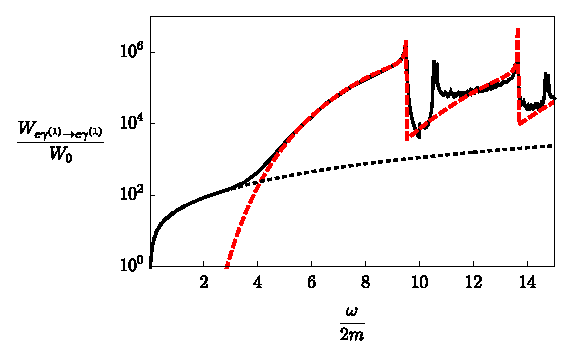
\includegraphics[width=0.8\linewidth]{Splot112001.eps}
	\caption{����������� ������������ ���������� �� ������� ���������� ������ ��� ������ $e\gamma^{(1)}\to e\gamma^{(1)}$ ��� ���� $B=200 B_e$ � ����������� T=1 ���: �������� ����� -- ����������� ���������� � ������ ���������; ��������� ����� -- ��� ����� ���������; ���������� ����� -- ������-�������������� �����������. ����� $W_0=(\alpha/\pi)^3m\simeq 3.25\cdot10^2$ ��$^{-1}$.}
	\label{Graph11B200T1}
\end{figure}

\begin{figure}[t!]\centering
	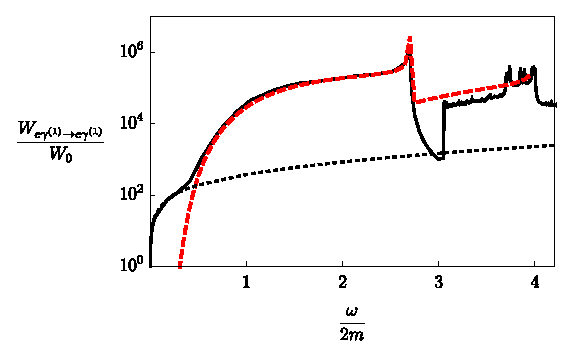
\includegraphics[width=0.8\linewidth]{Splot11201.eps}
	\caption{����������� ������������ ���������� �� ������� ���������� ������ ��� ������ $e\gamma^{(1)}\to e\gamma^{(1)}$ ��� ���� $B=20 B_e$ � ����������� T=1 ���. ����������� ��� ����� �� ��, ��� � ��� ���. \ref{Graph11B200T1}.}
	\label{Graph11B20T1}
\end{figure}

\begin{figure}[t!]\centering
	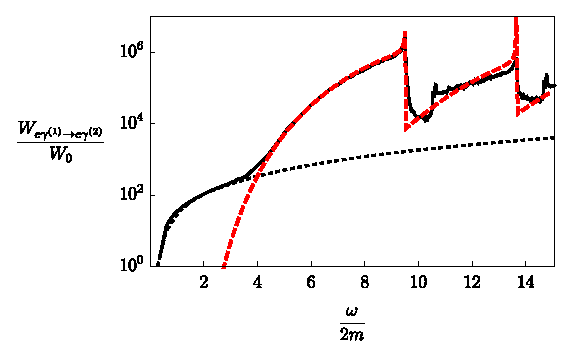
\includegraphics[width=0.8\linewidth]{Splot122001.eps}
	\caption{����������� ������������ ���������� �� ������� ���������� ������ ��� ������ $e\gamma^{(1)}\to e\gamma^{(2)}$ ��� ���� $B=200 B_e$ � ����������� T=1 ���. ����������� ��� ����� �� ��, ��� � ��� ���. \ref{Graph11B200T1}.}
	\label{Graph12B200T1}
\end{figure}

\begin{figure}[t!]\centering
	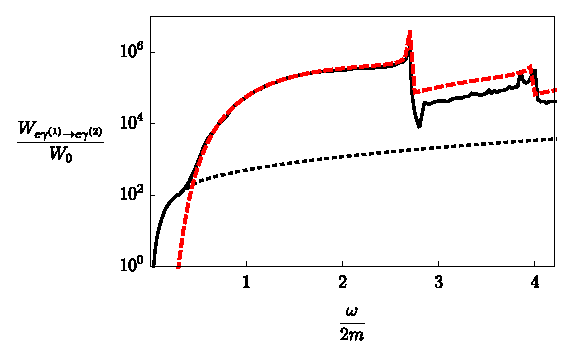
\includegraphics[width=0.8\linewidth]{Splot12201.eps}
	\caption{����������� ������������ ���������� �� ������� ���������� ������ ��� ������ $e\gamma^{(1)}\to e\gamma^{(2)}$ ��� ���� $B=20 B_e$ � ����������� T=1 ���. ����������� ��� ����� �� ��, ��� � ��� ���. \ref{Graph11B200T1}.}
	\label{Graph12B20T1}
\end{figure}
\clearpage



\section{������}
\label{sec1.5}
� ������ ����� ���������� ������������� ������� � ������ �������� ������ ���������� ���������. ���������� ������~\cite{RumShlenYar:2017} ��������� ������������� �������� ������������ ���������� ������ � ������������� �������� � ������-�������������� ����������� � ������������� ����������, ����������� � ���������� � ������ �������� ������. �����������, ��� ������-�������������� ����������� �������� ���� ������������ � ������� ��������� ���������� ���������� ����  \mbox{$B\simeq10^{12}-10^{13}$ ��} � ����������\linebreak $T\simeq 5-50$ ���, ����������� ��� �������������� � ����������, ���� �������� ����������� ����� ��������� ��� ���������� �����������.

��� ������ ������������� ����������� ������ ��� �����������\linebreak $T=1$ ��� � ������� ��������� ���� �������� ����������� ���������� ������ � ������������� �������� � ������ �������� ������ ������� ���������. ��������� ���������  ��������� ���������� ����������� � ������������� ���������� ��� ��� ����� ���������, ��� � � $\delta$-�������������� ������������ ��� ���� ��������� ��������� �����, ������� ����� ��������������� � ���������� �������� SGR: $B=20 B_e$ � $B=200 B_e$. ����������� ��������� ������� ���������� ���������� ��������� �������������� �������� �� �������� �������� ����~\cite{Rumyantsev:2017}. ������-�������������� ����������� � ����������� ��������� ��������� ������ ������ ����������� ���, ��������� ������� ������� ���������� ��� �� ������, ��� � �� ������. � ������ �������, � ����� ������ �������� ������ ���������� ������������, ��� �������� ����� ��� ���� ����������� ��������, ������� ��������� �� ������ ������ ������.



\newpage
\newpage
\chapter{��������� ������ � ������ ������������� ������}
\section{��������}
\label{sec2.1}

��� ���� ����������� � ������ �����, � ����������� ������ ������������� ����� �������� ��������� ������������� � ��������������� ������� ������. ���� ���� ����� ��������� � ������������ ���������� ���������� ���������, � ���������� �������, ��������, ���������� ���������� ����� �������, ��� ������������ �������� ��������-����������� ���� $\gamma\to e^+e^-$ ��� ���������� ������ $e^{\pm}\gamma\to e^{\pm}$, ������� ������������� ��������� ��� ��������� � �������. � ������ �������, ������ ���������� ���� ������� ��������� ������� �����, ��� ��� ����� ������ ������������ ����� � �������� ��������� ��������� ������ ��� ���������� ������������ ���������������� �����. ������� ������������ ��������� ������� ����������� ��� ������� ��������� ������ �� ���� ������� ���������� ������ ���������� (����������)
$\gamma e^{\pm} \to e^{\pm}$ � �������� ��������-����������� ��� $\gamma \to e^+ e^-$, ������� �������� ������� � ����������� ������������� ���������� �����~\cite{Kostenko:2018,Philippov_2020}. 

������� �������� ��������-����������� ����  � ��������� ���� � ��������� ����������� ��� ���������� � ���� �����~(��., ��������,~\cite{Klepikov:1954,Sturrock:1971,Tademaru:1973,Daugherty:1983,Shabad:1988}). ������, ��� �������������� � ������~\cite{Shabad:1988}, ���� ������� �������� �������������� � ����������� �������� $\gamma\to e^+e^-$ ���������, ��� ��� ������ ������� ������ ���������������� ��� ����������� ��������� ������ ������ ����������� ��������. ������� ��� ������� ���� ������ � ������~\cite{Shabad:1988} ������������ ���������� ����������� ��������� ������, ����� ��������� ��������� �� ������ ��������� �����.  ��� ���� �������� � ������~\cite{Chistyakov_gee:2001}, ����� ����� ����� ��� �����������. ��-������, ������� � ������������ ��������� ������ ��������� �� ������������ ��������� ������, ���������� ������� ������ ������ ����������. ��� �������� � ������������� ������������ ����� ������� ��������� ��������� ��� � ��������������, ��� � � �������������� ���������� ������ ����� �������. ��-������, � ������ ������ � �������������� ������� ������������� ���������������� �������� ��������� ���������������� �����, ���, ������ ������, �������� ������~\cite{Chistyakov_gee:2001}, �� ���. ������� � ������~\cite{Chistyakov_gee:2001} ��� ������������ ���������� ��������� ���������������� ����� �� ������� ��������� ���� ��� ���������� �����, ������� ����������� � ���������� �������������� ������� ��������� ����������������� ���� � ����������� �������� ��������� � ������ ����������� ������� �� ������� ��������� ����. � ������ �������, � �������~\cite{Shabad:1988,Chistyakov_gee:2001} ��������� ������ ��������������� � ��������� ����, ������ � ������ ������������� ������ ����� ������������ �� �����������, ����� ��� ��� ��������������� ���������� ������� ������������� ����� �������� �������� �����������.

� ������ ����� ��������������� ��������� ������ ��� ��������� ��������� $\gamma e^{\pm} \to e^{\pm}$ 
� $\gamma \to e^+ e^-$ � ������ ������������� ������ $\beta \gg T^2$ ��� ����������� $T \simeq 1$ 
��� � ������� ���������� ���������� $\mu = 0$. 
�� ���������� �����, ����������� � ������ ���� ��� �������� ������������ � � ������ ������~\cite{Boyan}, �������� �� ������ �������� ���������� ���� �~\cite{Chistyakov_gee:2001}. �� ������� �
���������� �������������� ������� ��������� ����������������� ���� ��� ������� �������� ��������� � ������ ����������� ������� � ������������� ������.

\section{��������������� ������ � ������������� �����}

��� �������� �������� ���������������� ����� ${\cal A}_{\alpha}(x)$, ��� $x_\mu = (t, {\bf x})$, 
�� ������� ������������� ���������, �������� ���������� �~\cite{Chistyakov_gee:2001} ��� ������ ���������� ����. ���������� �������� ������ ������� 
(${\cal A}_{\alpha}(x)$ � ������������� ������) �� ������� ��������, ������� ������������� ���������� 
��� $t = - \infty$ � � ������ ������� $t = 0$ �����������. ��� $t > 0$
���������������� ����� ����� ���������������� ��������������. �����
�������, �������� ��������� ��� �������� ���������� ���������. ��� �����
������� ��������� ����� ������� � ����:
%
\beq
{\cal J}_{\alpha}(x) = j_{\alpha}\,e^{i \,{\bf k} {\bf x}}\,
e^{ \varepsilon t}\, \theta(- t), \,\,\, \varepsilon \to 0^+,
\label{eq:1}
\eeq
��� $j_{\alpha} = (0, {\bf j}),\,\,{\bf j} \cdot {\bf k} = 0$ � ����� ���������� ����. ����� ���
�������� ���������� �������� ����������������� �����. ������ ������, � ������������� ������ ��-�� ������� ����������� ������� ������ � ��������������� ������ ��� ������������ ����� � ���������� ���� ������������ ������������ ���������. ������� � �������� ��������� ���������� ������� ������, ����� ������ ���������������� ������� ���������� ���� ���, ��� $k_z=0$. ����������� ${\cal A}_{\alpha}(x)$ �� �������  ������������ ����������
%
\begin{eqnarray}\label{eq:WaveEq}
%\nonumber
%&& 
(g_{\alpha \beta} \, \partial_{\mu}^2  -
\partial_{\alpha}\partial_{\beta}) \, {\cal A}^{(\lambda)}_{\beta}(x) + 
%\nonumber \\
%&&+ 
\int d^4 x'\, {\cal P}^{(\lambda)}_{\alpha \beta} (x - x') \, {\cal A}^{(\lambda)}_{\beta}(x')
= {\cal J}_{\alpha}(x),
\label{eq:2}
\end{eqnarray}
%                                                                                         \frac{(\varphi q)_\mu}{\sqrt{q^2_\perp}}
��� ${\cal P}^{(\lambda)}_{\alpha \beta} (x - x')$ -- ��������������� �������� ������ � ��������� ���� � ������. $q^{\mu} = (q_0,\, {\bf k})$ -- 4-������ �������� ������.

% ������� ��������, ��� � ����� ������ ��������������� �������� ������� �� ������ ���������� $x$ � $x'$ � �����������. ������, ���� ��������������� �������� �� ���������� ����� ����������� � ��������, �� ����� � ����� ������ ����� ������� ����������. ����� ��������������� �������� ����� �������� �� �������� $x-x'$.

������������� ������� ���������~(\ref{eq:WaveEq}) ����� ����������� � ��������� ����:

\begin{equation}\label{eq:RetSol}
	{\cal A}^{(\lambda)}_\alpha(x)=\int \dd^4 x' G^R_{\alpha \beta}(x-x'){\cal J}_\beta(x')\, ,
\end{equation}
��� $G^R_{\alpha \beta}(x-x')$ -- ������������� ������� ����� (��., ��������~\cite{Landau:2001}).

������ ������~\cite{Chistyakov_gee:2001}, ���������� �������� ��������� � ��������� ���� ������������� ��������� ������������ ����� ������������� $G^R_{\alpha\beta}(x-x')$ � ��������� $G^C_{\alpha\beta}(x-x')$ ��������� �����:

\begin{equation}\label{eq:RetCasualGreen}
G^R_{\alpha\beta}(x-x')= 2 \mathrm{Re} G^C_{\alpha\beta}(x-x')\theta(t-t')\, .
\end{equation}

\begin{center}
	\begin{figure}[t!]\centering
		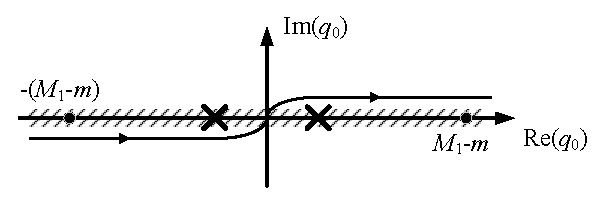
\includegraphics[scale=1.5]{PathIntegrateMode1.eps}
		\caption{������ �������������� �� $q_0$ �~(\ref{eq:FullIntegrate}) ��� ���� 1. �������� �������� ������� �������������� ������. ��������� ��������� �����, ��������������� $q_0=\omega$ -- ������������� ������������ �������� ���������������� ���������, ������� ���������� ������.} \label{fig:FullPathIntegrMode1}
	\end{figure}
\end{center}

���������� ���������� ���� �������� ������� ����� �� ����������� �������� $r_\alpha^{(\lambda)}$ ���������������� ��������� � ������������� ������ (��. ����������~\ref{app3}):
\begin{equation}\label{eq:InvGcFourier}
	G^C_{\alpha\beta}(x)=\int \frac{\dd^4q}{(2\pi)^4}G^C_{\alpha \beta}(q) e^{-\ii qx}\, ,
\end{equation}
\begin{equation}\label{eq:GcFourier}
	G^C_{\alpha\beta}(q)=\sum_{\lambda=1}^{3}\frac{r_\alpha^{(\lambda)}r^{(\lambda)}_\beta}{(r^{(\lambda)})^2}\cdot \frac{1}{q^2-{\cal P}^{(\lambda)}(q)}\, ,
\end{equation}
��� ${\cal P}^{(\lambda)}(q)$ -- ����������� �������� ���������������� ��������� � ������������� ������.

�����, ���������� ���������~(\ref{eq:RetSol}) � (\ref{eq:WaveEq}) � ������~(\ref{eq:RetCasualGreen})--(\ref{eq:GcFourier}), ������� ��������� ���������:
\begin{equation}
	A^{(\lambda)}_\alpha(x) = 2 e^{i \mathbf{kx}} \mathrm{Re} \sum_{\lambda=1}^3 \int\frac{\dd q_0}{2\pi i}\frac{r_\alpha^{(\lambda)}(r^{(\lambda)} j)}{(r^{(\lambda)})^2}\frac{e^{-i q_0 t}}{(q_0-i\varepsilon)(q_0^2-\mathbf{k}^2-{\cal P}^{(\lambda)}(q))}
\end{equation}


������� ���������~(\ref{eq:2}) ��� ������� ��� $\lambda = 1,2$ ������ ����������� � ����:
%
\begin{eqnarray}                        		
{\cal A}^{(\lambda)}_{\alpha} (x) = V^{(\lambda)}_\alpha (0, {\bf x}) \, \text{Re} F^{(\lambda)} (t) \, ,
\label{eq:V}
\end{eqnarray}
��� 
%
\begin{eqnarray}
V^{(\lambda)}_\alpha (0, {\bf x}) = 2\, e^{ i\, {\bf k x}} \, 
\varepsilon^{(\lambda)}_\alpha \, (\varepsilon^{(\lambda)} j)\, .
\label{eq:partialV}
\end{eqnarray}
%
%\beq
%V^{(2)}_\alpha (0, {\bf x}) = 2\, e^{ i\, {\bf k x}} \, \varepsilon^{(2)}_\alpha \, \frac{(q \tilde \varphi j)}{\sqrt{q^2_{\mprl}}} \, .
%\label{eq:partialV2}
%\eeq
%��� ����������� �������, ������ �������������� ������
%������������� � ������, ������������ �� ���.11. 

\newpage ������� $F^{(\lambda)} (t)$ ������ ����������� � ���� �����-���������

\begin{equation}\label{eq:FullIntegrate}
	F^{(\lambda)}(t)=\int_C\frac{dq_0}{2\pi \ii}\frac{e^{-\ii q_0 t}}{(q_0-\ii \varepsilon)(q_0^2-\vec{k}^2-{\cal P}^{(\lambda)}(q))}.
\end{equation}

	\begin{figure}[t]\centering
		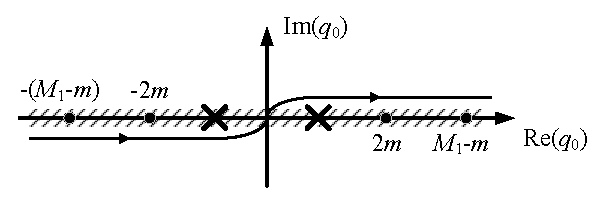
\includegraphics[scale=1.5]{PathIntegrateMode2.eps}
		\caption{������ �������������� �� $q_0$ �~(\ref{eq:FullIntegrate}) ��� ���� 2. �������� �������� ������� �������������� ������. ��������� ��������� �����, ��������������� $q_0=\omega$ -- ������������� ������������ �������� ���������������� ���������.}\label{fig:FullPathIntegr}.
	\end{figure}

������ �������������� $C$ ������������ �������� ������������� ��������� ���������������� ���������. ����� �� ���� ������������ �������� ����� $q_0=\omega$, ������� ������������� ��������� ��������� \begin{equation}
	\omega^2 - \vec{k}^2 - {\cal P^{(\lambda)}}(q)=0.
\end{equation}

� ������ �������, ����������� �������� ���������������� ��������� ������ ������� $q_{\mprl}^2=(M_n\pm M_\ell)^2$, ���������� � ����� 1, ����� ����� �������, ������� ������� � �������� ������ �� $e^+e^-$-���� � ��������� ��������� �� ������ ������ ������, �. �. ������������� �������� �������������� ������, ������� ������� ������� �� ���.~\ref{fig:FullPathIntegr}. � ������ ���� ������������  ������ �������������� ����� ���� ���������, ��� �������� �� ���.~\ref{fig:FullPathIntegr}.

� �������������� ������� $\omega<2m$ ������ ����� ���������������� ��������� ��� ����� ��� ������������ ���� �� ��������� � �������� ������ (������� ��������� �����������), ������� ��� �������� ������ �������������� � ��� ������ ���� 2, � ��� ������ ���� 1 ����� ������������� �������� ���.~\ref{fig:PathIntegrMode2}  � ���.~\ref{fig:PathIntegr}. ����� �������, ��������~(\ref{eq:FullIntegrate}) ����� ����������� � ���� ���� ���������
\begin{eqnarray}
F^{(\lambda)}(t) = F^{(\lambda)}_{pole}(t) + F^{(\lambda)}_{cut}(t),
\label{eq:19}
\end{eqnarray}
%
������ �� ������� ������������ ������� � ����� $q_0 = \omega$, ����������
�������� ��������� ��������� $q^2 - {\cal P}^{(\lambda)}(q) = 0$ � �������������� �������, ��� ����������� 
�������� ���������������� ��������� ������ ${\cal P}^{(\lambda)}(q)$ -- �����������. 

%��� ������������� �������������
%������� � ������� $\omega < 2 m$~\cite{Shab}.
������ ��������� ���������� ����������� ����������������� ���� �� �������
� ������� $\omega>2m$ � ����� ���
�����-���������:
%
\begin{eqnarray}
F^{(\lambda)}_{cut}(t) &=& \int \limits_{- \infty}^{\infty} \frac{dq_0}{2 \pi}\,
F^{(\lambda)}_{cut}(q_0)e^{- i q_0 t},
\label{eq:20} 
\\
F^{(\lambda)}_{cut}(q_0) &=& 
\frac{2 \,\theta (q_0  -  2 m)\,I^{(\lambda)}}
{q_0\,([ q_0^2 - {\bf k}^2 - R^{(\lambda)}]^2 + [I^{(\lambda)}]^2)},
\label{eq:21}
\end{eqnarray}
%
��� $R \equiv \text{Re} {\cal P}^{(\lambda)}(q_0)$  � ��������, $I \equiv  - \text{Im} {\cal P}^{(\lambda)}(q_0 + i \varepsilon)$ � ������ 
����� ���������������� ��������� ������ � ������������� ������. ������ �������������� ������� �� ���.~\ref{fig:PathIntegrMode2} � \ref{fig:PathIntegr}.

\begin{figure}[t]\centering
	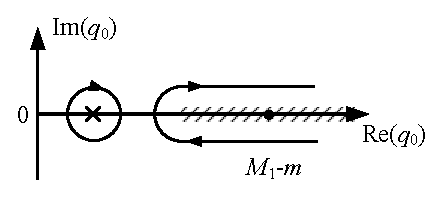
\includegraphics[scale=1.5]{PathIntegrate3Glmode1.eps}
	\caption{������ �������������� �� $q_0$ �~(\ref{eq:20}) ��� ���� 1. ��������� ������ �������� �������, ��� ������ ����� ���������������� ��������� �����������. ��������� ����������� ����������~���.~\ref{fig:FullPathIntegr}.}\label{fig:PathIntegrMode2}
\end{figure}

������ ����� ���������������� ��������� ����� ���� �������� �� ������������  
���������� ������
\begin{eqnarray}
W^{(\lambda)}_{abs} = W_{\gamma^{(\lambda)} \to e^+ e^-} + W_{\gamma^{(\lambda)} e^{\pm} \to e^{\pm}} \, .
\label{eq:Wabs}
\end{eqnarray}

\begin{figure}[t]\centering
	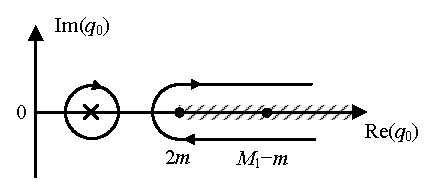
\includegraphics[scale=1.5]{PathIntegrate2Gl.eps}
	\caption{������ �������������� �� $q_0$ �~(\ref{eq:20}) ��� ���� 2. ��������� ������ �������� �������, ��� ������ ����� ���������������� ��������� �����������. ��������� ����������� ����������~���.~\ref{fig:FullPathIntegr}.}\label{fig:PathIntegr}
\end{figure}

� ������ ��������� ��������� �������, (\ref{eq:Wabs}) ����� ���� ������������ � ��������� ����� (��., ��������,~\cite{Shabad:1988, Rumyantsev:2017,Weldon:1983}): 
\begin{eqnarray}
\text{Im} {\cal P}^{(\lambda)} =  -2 q_0 [1-\exp (-q_0/T)] W^{(\lambda)}_{abs} \, . 
\label{eq:ImP}
\end{eqnarray}

�������� $W_{\gamma^{(\lambda)} \to e^+ e^-}$ ����� ���� �������� ��~(\ref{eq:wabs1}) �~(\ref{eq:wabs2}) 
� �������������� ������������ ���������:
\begin{equation}
	\begin{gathered}
		W_{\gamma^{(1)}\to e^+e^-}= \frac{\alpha\beta }{\sqrt{q_0^2}}\sum_{\ell, \ell'=0}^{\infty}\frac{[1-f_{E_{\ell}}][1-f_{\omega-E_\ell}]}{\sqrt{\left( M_{\ell'}^2-M_\ell^2-q_0^2\right)^2-4q_0^2 M_\ell^2}}\times
		\\
		\times \left\{\left(2\beta  ({\ell'}+\ell)-q_0^2\right)\left({\cal I}_{{\ell'},\ell-1}^2+{\cal I}_{{\ell'}-1,\ell}^2\right)-
		8 \beta  \sqrt{l n} {\cal I}_{{\ell'},\ell} {\cal I}_{{\ell'}-1,\ell-1}
		\right\}\, .
	\end{gathered}
\end{equation}
	
	\textcolor{red}{������ �������, ��� ��� ������ ���� 1 ����������� ���������� � �������� �������� ��������-����������� ���� � �������� ������ $\ell=\ell'=0$ ����� ����. ��� ������ ���� 2 ����� ������� ��� ��� �� �������� ���������� ��������}:
\begin{equation}
\begin{gathered}
%W_{\gamma^{(2)}\to e^+e^-}=\frac{\alpha\beta}{2}\frac{1}{M_{\ell'}q_0^2}\frac{1}{q_0\sqrt{(q_0^2-(M_\ell^2+M_{\ell'}^2))^2-4M_\ell^2M_{\ell'}^2}}\frac{1}{q_0^2-(M_\ell+M_{\ell'})^2}\times
%\\
%\times\bigg(
%(q_0^2+(M_\ell^2-M_{\ell'}^2))^2 M_{\ell'}(M_\ell^2+M_{\ell'}^2+2m^2)
%-
%2M_\ell (M_\ell+M_{\ell'})^2(m^2+3M_\ell M_{\ell'})q_0^2\bigg)\times
%\\
%\times[{\cal I}_{\ell,\ell'}^2+{\cal I}_{\ell-1,\ell'-1}^2] - 4M_{\ell'} q_0^2 (q_0^2-(M_\ell+M_{\ell'})^2)2\beta \sqrt{\ell \ell'} {\cal I}_{\ell\ell'} I_{\ell-1,\ell'-1}\\
W_{\gamma^{(2)}\to e^+e^-}= \frac{\alpha\beta }{\sqrt{q_0^2}}\sum_{\ell, \ell'=0}^{\infty}\frac{[1-f_{E_\ell}][1-f_{\omega-E_\ell}]}{\sqrt{\left( M_{\ell'}^2-M_\ell^2-q_0^2\right)^2-4q_0^2 M_\ell^2}}\times
\\
\times \left\{\left(\frac{\left[2\beta  ({\ell'}-{\ell'})\right]^2}{q_0^2}-2 \beta  (\ell+{\ell'})-4m^2\right)\left({\cal I}_{{\ell'},\ell}^2+{\cal I}_{{\ell'}-1,\ell-1}^2\right)-
8 \beta  \sqrt{\ell {\ell'}} {\cal I}_{{\ell'},\ell} {\cal I}_{{\ell'}-1,\ell-1}
\right\}\, .
\end{gathered}
\end{equation}

��������, ��� ${\cal I}_{n, \ell}\equiv{\cal I}_{n, \ell} (\frac{q_\perp^2}{2\beta})$.

�������� ����� 
���������������� ��������� ����� ���� ������������� �� ��� ������ ����� � ������� �������������� ����������� � ����� 
����������:
%
\beq 
{\cal P}^{(\lambda)} (t) = \int \limits_0^\infty \frac{Im({\cal P}^{(\lambda)} (t'))\,dt'}{t'-t-i o} - {\cal P}^{(\lambda)} (0)\,, \qquad  t = q^2_0 \, .
\label{eq:Disp}
\eeq



� ���������� ��������� ��� ������ � �������������� ������ ���������������� ��������� ��� ���� 1 � ������ �������� $\gamma^{(1)}e_0\to e_1$ ����� ����������� ��������� �������:

\begin{equation}
I^{(1)}=2\alpha\beta\exp \left[-\frac{q_\perp^2}{2\beta }\right]\frac{\left(2\beta -q_0^2\right) \left(f_{E_0}-f_{q_0-E_0}\right)}{ \sqrt{\left((M_1-m)^2-q_0^2\right) \left((M_1+m)^2-q_0^2\right)}}
\end{equation}

\begin{equation}\begin{aligned}
R^{(1)}&= -\frac{\alpha \beta}{2\pi}\exp\left[\frac{-q_\perp^2}{2\beta}\right]\bigg(\frac{2\beta-q_0^2}{\sqrt{((M_1+m)^2-q_0^2)((M_1-m)^2-q_0^2)}}
\times
\\
&\times
\ln\left[\frac{\sqrt{(M_1+m)^2-q_0^2}+\sqrt{(M_1-m)^2-q_0^2}}{2(m^4+2 \beta m^2)^{1/4}}\right]-\ln\left[1+\frac{2\beta}{m^2}\right]\bigg)
-
\\
&-\frac{\alpha \beta q_0^2}{2\pi} \exp\left[-\frac{q_\perp^2}{2\beta}\right]\int_{0}^{\infty}\frac{8m^2\sqrt{z^2+1}}{\left(\exp \left(\frac{\sqrt{z^2+1}}{T/m}\right)+1\right) \left(\left(2\beta-q_0^2\right)^2-4m^2q_0^2 \left(z^2+1\right)\right)}\dd z\, .
\end{aligned}
\end{equation}

� ������ �������, ��������������� �������� ��� ������ ���� 2 � ������ ��������� $\gamma^{(2)}e_0\to e_1$ � $\gamma^{(2)}\to e^+_0 e^-_0$ ������ ���:
\begin{equation}\begin{aligned}
I^{(2)}=&2\alpha\beta\left[1-\exp\left(\frac{-q_0}{T}\right)\right]\exp\left[{\frac{-q^2_\perp}{2\beta}}\right]\Bigg\{\frac{[1-f_{E_0}][1-f_{\omega-E_0}]}{\sqrt{(q_0^2)^2-4q_0^2m^2}}4m^2+
\\
+ &\frac{f_{E_0}\left[1-f_{\omega-E_1}\right]}{\sqrt{((M_1-m)^2-q^2_0)((M_1-m)^2-q^2_0)}}\left(4m^2+2\beta-\frac{(2\beta)^2}{q_0^2}\right)\Bigg\}\, ,
\end{aligned}\end{equation}

\begin{equation}\begin{aligned}
	R^{(2)}&= \frac{\alpha\beta}{2\pi}\exp\left[-\frac{q_\perp^2}{2\beta}\right]\left(\frac{4m^2}{\sqrt{q_0^2(q_0^2-4m^2)}}\ln\left[\frac{\sqrt{q_0^2}+\sqrt{q_0^2-4m^2}}{4m^2}\right]+1\right)+ 
	\\
	&+\frac{\alpha}{16\pi}q^2_\perp \exp\left[-\frac{q_\perp^2}{2\beta}\right] \bigg( \frac{4m^2+2\beta+\frac{4\beta^2}{ q_0^2}}{\sqrt{((M_1-m)^2-q^2_0)((M_1-m)^2-q^2_0)}}
	\times
	\\
	&\times
	\ln\left[\frac{\sqrt{(M_1+m)^2-q_0^2}+\sqrt{(M_1-m)^2-q_0^2}}{2(m^2+2\beta)^{1/4}}\right]+
	\\
	&+\frac{1}{2}\left(\frac{m^2}{\beta}-\frac{2\beta}{q_0^2}\ln\left[\frac{m^2+2\beta}{m^2}\right]+1\right)\bigg)-
	\\
	&- \frac{2\alpha\beta m^2}{2\pi}\exp\left[-\frac{q_\perp^2}{2\beta}\right]\int_{0}^{\infty}\frac{1}{\sqrt{1+z^2}}\frac{1}{\exp[\frac{\sqrt{1+z^2}}{T/m}]}\bigg(\frac{1}{q_0^2-m^2(1+z^2)}+
	\\
	&+\frac{2\beta z + q_0^2}{(2\beta - q_0^2)^2-m^2(1+z^2)q_0^2}\bigg)\dd z\, .
\end{aligned}\end{equation}

������� ��������, ��� � ������������ ������ ��������������� �������� ������ �� ������� ������������� ��������� $\omega=M_1-m$, ������� �� �� �������� � ������� �������� ������ ������ �� ����.

��������� (\ref{eq:20})-(\ref{eq:Wabs}) � ������ (\ref{eq:Disp}) ������ ������ 
� ���������� ��������� ����������� �������� ������� ������  � ����������� ������ 
������������� ������. 

\begin{figure}[t]\centering
	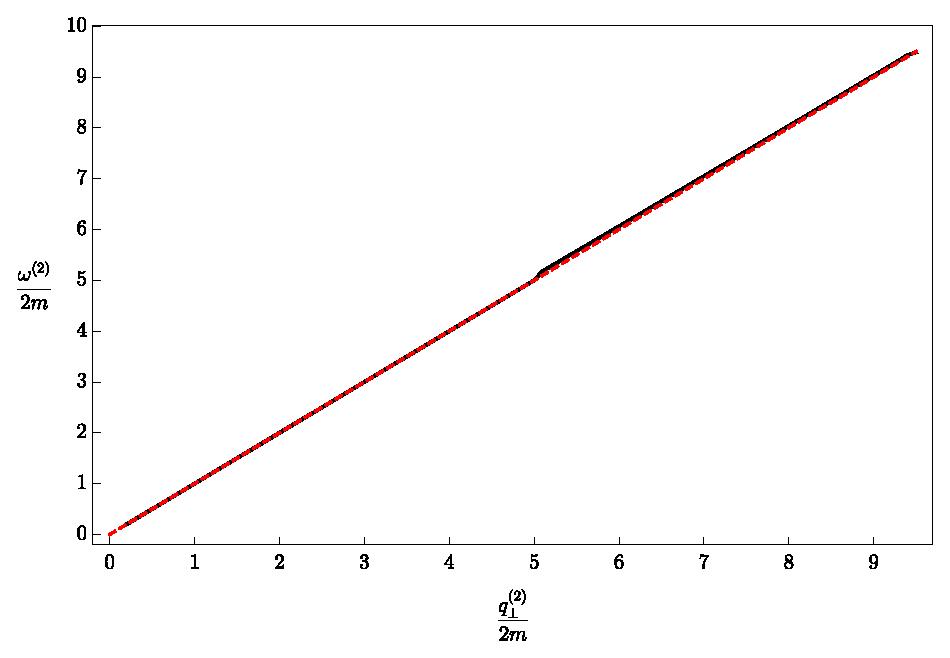
\includegraphics[scale=0.8]{DisperseMode1.eps}
	\caption{��������� ������ ���� 1 � ������� ��������������, ��������� � ��������� ���������� $e_0 \gamma^{(2)}\to e_1$ ������������ �������� ������ ��� ��������� ���� $B=200B_e$ � $T=1$~���. ��������� ����� ������������� ���������� ������ ���������.\label{fig:DisperseMode1}}
\end{figure}

��������� ����� �������� ������� ������ $F(t)$ ����� ����������� � ���� ���������� ���������:
\begin{equation}\label{eq:Fm}
	F(t)\sim F_A(t) \cos(\omega^{(\lambda)} t+\phi_0)
\end{equation}
��� $F_A(t)$ -- ��������� ���������,
��������� ����������� ������� ����������
�������� ��������� �������� �������,
$\omega^{(\lambda)}$ -- �����������
�������. � ������~\cite{Shabad:1988}
������������� ���������������� �������� ��������� � ����������� ���������, ������ ������ ����� ������� ������, ���������� �� ������� ��������� ��������� �� ������ ��������� �����. ������  ������������� ������� �����-������ $F^{(\lambda)}_{cut}(q_0)$ ����������, ��� �������� ���������� ��������� �������� ������� � ����� ������ �������� ������������������. ��� �� ����� �� ���������� ���������� ������������ ������� ������� $(\sim [W^{(\lambda)}_{abs}]^{-1})$
����������� �������� ������� �� ������� ����� ����������� ������� ��� 
��������������� ���������� ������������� ���������:
%
\begin{equation}\label{eq:ApproxA}
{\cal A}^{(\lambda)}_\mu(t) \sim e^{- \gamma^{(\lambda)}_{\mbox{\tiny eff}} \, t/2} \cos 
(\omega^{(\lambda)} t + \phi_0).
\end{equation}
%
����� $\omega^{(\lambda)}$ � $\gamma^{(\lambda)}_{\mbox{\tiny eff}}$ -- ����������� 
������� � �����������  
���������� ������ ���� $\lambda$ ��������������, ������� ������ ���� ������� � �������������� 
(\ref{eq:20})-(\ref{eq:Wabs}) ��� ������� �������� �������� ${\bf k}$, ��� ���������� ����������� 
����� ��������� ������ � ������� ��� ��������������~(��. ���.~\ref{fig:DisperseMode1} � \ref{fig:DisperseMode2}).

\section{��������� ������}

��� ��������������� ���������� ������� ��������� �������� $\gamma_{\mbox{\tiny eff}}$, ������� ���������� ������������� ���������� 
$\gamma$-������� � ������������� ������ �� ����  ��������� $\gamma \to e^+ e^-$  � $\gamma e^{\pm} \to e^{\pm}$.
������ � �����������  ���������� ��������� ��� ������������ ����������,
���������� �� ������  ����������� �������  $ \gamma \to e^+ e^-$. ������ � �������������� ������� ��� ���������
�������� �������� ������������� (��. ��������~\cite{HBG:1997}), ������� ���� �������� �� �������� ������� �������. 

	\begin{figure}[t!]\centering
		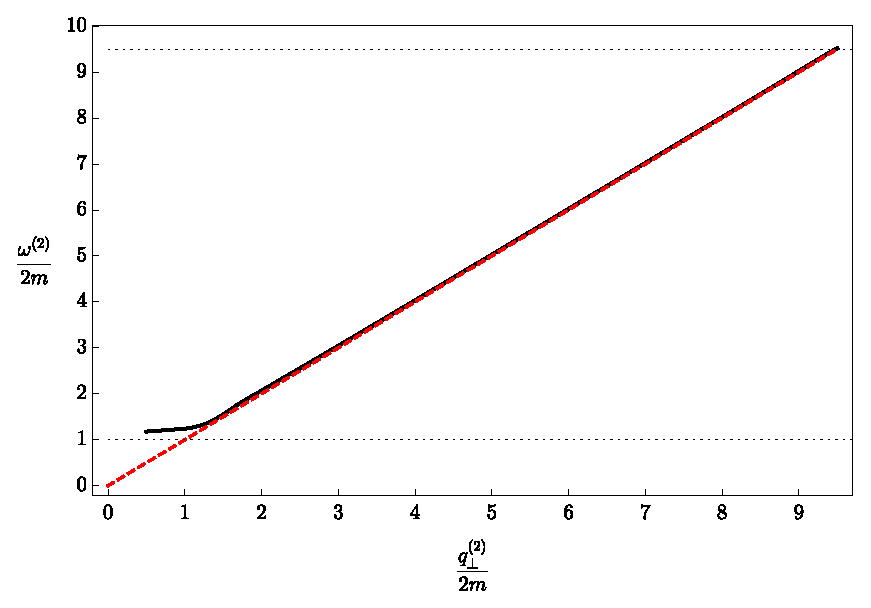
\includegraphics[scale=1]{DisperseMode2.eps}
		\caption{��������� ������ ���� 2 � ������� ��������������, ��������� � ���������� ������� �� $e^+e^-$ ���� � ���������� $e_0 \gamma^{(2)}\to e_1$ ������������ �������� ������ ��� ��������� ���� $B=200B_e$ � $T=1$~���. ��������� ����� ������������� ���������� ������ ���������. �������� ����� ���������� ������� $4m^2$ � $\omega=M_1-m$. \label{fig:DisperseMode2}}
	\end{figure}

��� ������ ����������, (��. ���.~\ref{fig:DampMode1} �~\ref{fig:DampMode2}),
��� ���������� ������������  ���������� � ������ ������������������� ��������� 
��������� �������� � ��������� ��������� ��� ������������  ���������� ������ � ����������� ���������� 
$q^2_0 = (\sqrt{m^2+2 eB} - m )^2$ ��� ��� ������ ���� 2, ��� � ��� ������ ���� 1. ������ �� ���. \ref{fig:DampMode1} ����� ������� �����, ��� ����� ���� 1 �������� ��������������� � �������� $q_0<7$ ��� � $q_0^2>(\sqrt{m^2+2 eB} - m)^2\simeq 9.5$~���. � ������ �������, ����� ���������� � �������, ������� � ����������� ���������� $q_0^2 = (\sqrt{m^2+2 eB} - m )^2$. ����� ���� 2 ����� ������� ��������������� � ������� $q^2_0<4m^2$ � $q^2_0>(\sqrt{m^2+2 eB} - m )^2$. ����������� ��������� ������, ���������� �� ����������� ������~\cite{Shabad:1988}, �������� ���������� � �������������� ������� �� ��������� � ������������, ����������� � ������� �������������~(\ref{eq:ApproxA}). ������ ���������� ������� ������� ������ ($2.5\lesssim q_0\lesssim 8.5$ ��� ��� ������ ���� 2 � $q_0\lesssim8.7$ ��� ��� ������ ���� 1), ��� ������������ ����������, ���������� �� ����������� ������~\cite{Shabad:1988} � � ������� �������������~(\ref{eq:ApproxA}) ���������.

\begin{figure}[t]\centering
	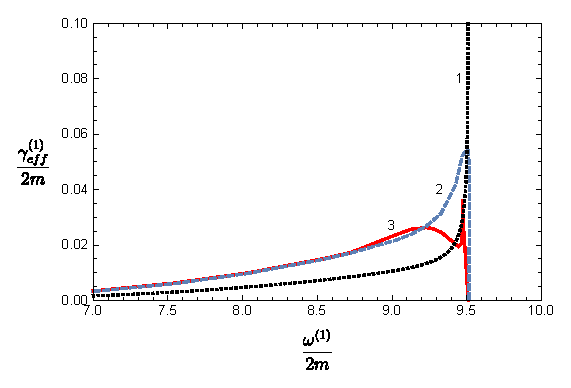
\includegraphics[scale=1]{mode1.eps}
	\caption{\label{fig:fig1}����������� ������ ������� ������ ���� 1 �� ������� � ������������ �������� ��� $B=200 B_e$, $T=1$ ��� � $ \mu=0 $. ����� $ {\it 1} $ - ����������� ���������� ������ $ W ^ {(1)}_{abs} $,
		% � ��������� $ \ gamma \ to e ^ + e ^ - $ � $ \ gamma e ^ { \ pm} \ to e ^ {\ pm} $,
		����������� � ��������� ����������� � ���������� �������� �����������; ����� $ {\it 2} $ - ������ �������, ���������� �� ������������ ������� �������������� ��������� �� ������ ��������� ����� [6]; ����� $ {\it 3} $ ������������� ������ ��������� $ \gamma^{(1)}_{\mbox {\scriptsize eff}} $, ����������� �� ������ �����������~(\ref{eq:ApproxA}).}\label{fig:DampMode1}
\end{figure}

 ���.~\ref{fig:DisperseMode1} � ~\ref{fig:DisperseMode2} ������������� ������ ��������� ������� ���� 1 � ����~2 � ������ ������������� ������ ��� ����������� $T = 1$ ��� � ��������� ���� $B = 200B_e$ � ������� �� ��������������. �� �������������� ����������� �������, ��� ����� ��������� ��� ������ ���� 1 � ������� �������������� ������������� ���������� �� ���������� ������ ���������~(��.~���.~\ref{fig:DisperseMode1}). � ������ �������, ������������� ������ ������ ���� 2 ����������� ���������� �� ��������� ������ ������ $q_0^2=4m^2$ � � ����� ����������� ������~$q_0^2=(M_1-m)^2$. ��� ���������� ������������� ������ �� ���������� ��������� ���������� ��������� ��������� ������ ������. ��� ���� ���������� ������� ������������� ������ ����������� � �������� ��������� ���������, ������������ � ������~\cite{Shabad:1988}.

�� ������ ���������� ����������� ������������ ������� ����������� ������ � ����������� ������������ �������������� �������� ��� ������� ��������� ������. ��� ����� ������ ��������� ��������� ������������ ��������� ������ ���� 1 � ������������ ���������� ������ � ������������� �������� $e\gamma^{(1)}\to e\gamma$ (��. ���. \ref{fig:ComptonandDamp}). ��� ����� �� �������~\ref{fig:ComptonandDamp}, ������������� �������, �������� �� ����� ������ $\alpha^2$, �������� ������������� ��� �������� ������ $q_0\lesssim3$ ���. ��� ������ ���� 2 ������������� ������� ����������� � ������� ������� ������ $q_0\lesssim1$ ���. � ������� ������� $q_0>3$ ��� (��� ���� 1) � $q_0>1$ ��� (��� ���� 2) ������ ����� ���������� ��������, � ������������� �������, ��-��������, �� �������� ��������������.
	\begin{figure}[t]\centering
	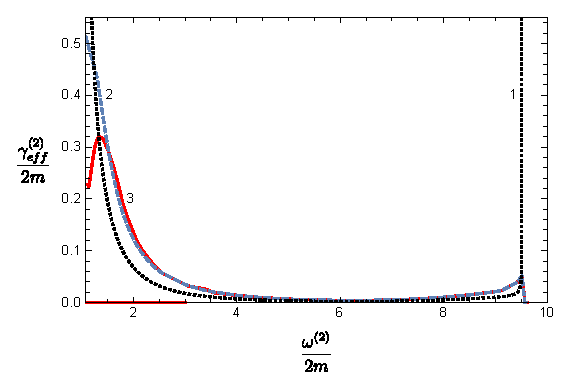
\includegraphics[scale=1]{mode2.eps}
	\caption{\label{fig:fig2} ����������� ������ ������� ������ ���� 2 �� ������� � ������������ �������� ��� ��� �� ���������� � �����������, ��� � �� ���.~\ref{fig:fig1}.}\label{fig:DampMode2}
\end{figure}


\section{������}
���������� ������� ��������������� ���������������� ����� � ������ �������������, ��������-������������ ������. � ������ ��������� ������������� ������� ������ � ��������� ���� � ������ ���� �����������, ���, ���������� ������ ������� ���������� ���� ������� ��������� ������
� ������������� ������ ����� ������������������ ��������. ��� ����������� ��������� ��������� ������ ���������� ��������� ����� ��������� ������ ��������� ����������� ��������� $F_m(t)$ ���������, �������� � ���������~(\ref{eq:Fm}).

��� ������������ ������� ������� $\sim [W^{{(\lambda)}}_{abs}]^{-1}$ ���� ������������ ������������� ��������������� ����������� �����������. � ���� ������ ����
��������, ��� ����������� ���������� ������ � �������������� ������� ������ �� ��������� � ���������� � ���������� ������������. �����, ������ ������ �������������, ���� ��������� ������������� ������, ������� � ��� ���� 1, � ��� ���� 2 ������ � ��������� ������. ����� ������� ����������� � ������������ ������~\cite{Shabad:1988}.

����� ����, ��� �������� ������ ����������� ������������ �������������� �������� � �������� �������������� ������ �� ���� �������� ���������� ���������� $e^\pm\gamma\to e^\pm$ � ������� �� ��������-����������� ���� $\gamma\to e^+e^-$. �������� �� ����� ������ $\alpha$, ������������� ������� ����������� ��� ���������� ������� � ���������� � ������� ������ ������� ������ ($\omega<3$ ��� ��� $T=1$ ��� � $B =200B_e$). � ������ �������, ���� � ������ ��������� �� ����������� ���������, ������ ��� ���� 1, ��� � ���� 2 � ������� �������� ���������� ���� $B=200 B_e$ � ����������� $T=1$ ��� ���������� �������� � ����������� �������.

		\begin{figure}[t!]\centering
			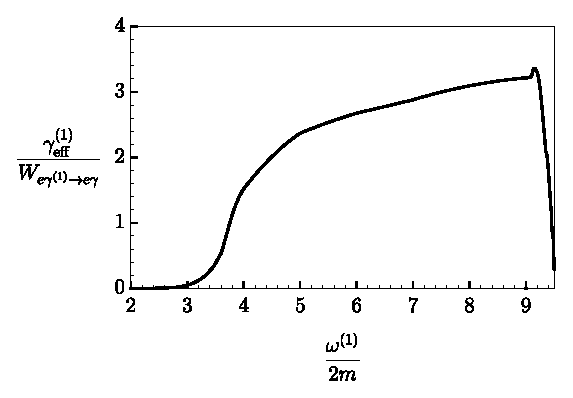
\includegraphics[scale=1]{CompareDampAndCompton.eps}
			\caption{\label{fig:ComptonandDamp} ��������� ������������ ��������� ������ $\gamma_{eff}^{(1)}$ � ������������ ���������� ������ � �������� $e\gamma^{(1)}\to e\gamma$ ��� $B=200B_e$ � $T=1$ ���}
		\end{figure}
\newpage
\newpage                                                                                                              
\chapter{������� ������������� ��������� � ������ ������������ �������������� ���������}
\label{sec:intro}

\section{��������}

%��-�� �������� ��������� ������������ ���������� ������ � ������������� �������� ������ ��������� ������ � �������� ��������� ���������� �������������.
%������������ �������� � ������� ���� ������ ��� ������ ������������� ������ ��� ��������� � ��������� �����������~\cite{Nagel:1981}, ��� ���� ��������, ��� ������������ ��������� �������� � ������� ���������� � ������� ���������, ������� ����������� ������� �� ����������� � ��������� ������. ���������� ���� ��� ����������� �����, ��� � �������� ������������� (������������� ������������� ���������) � ������~\cite{Meszaros:1985} �������, ��� ��������������� ��������� ������ ���������� ����������� ������ �� ��������� � ����� ���������, ������ �����������. ����������� ����� ��� ����������� � � ������~\cite{Kaminker:1982} � ����������� �������� ������ ($T\ll m$) � ������ ����������� ������� ��� ������, ����� ����������� ������������� ��������� �������� ������������. � ������~\cite{Alexander:1989} ���� ������� ��������� ������ ��� ������� ������ �������� � ������ ������ ����������� ������� ��� �������������� ����������� ������������� ���������, ������� ����� ������� ������������ ����� � ����������� ���������� ������.  ��� ������������ �������� ����������, ��������� ������ � ���������� ���� ���������� ������� ������������ ����������� � ���� �����~\cite{Burnard:1990,Meszaros:1983,Harding:1984,Nishimura:2015}. 
���� ��������� �������� ������� ������ �������� ���������. ���� �� ��� ����������� � ������� ������� �������-���������������� ���������, ��������������� ��������� ���������. � �������~\cite{Nagel:1981,Kaminker:1982,Meszaros:1985,Alexander:1991,Nishimura:2008} ��� ������� ������� ��������� �������� ������������� ��������� �����, ������� ����������� � ���, ��� �����������-���������������� ��������� ������������� � ������� ���������� ��������� � ������������ ���� � ������������������� �����������, ������� ����� �������� ������� ������~\cite{Mihalas:1985}.

� ������ �������, ��� ������� ������ �������� ��������� � ������ ������������ �������������� �������� ����� ������� ������������ ����� �����-����� (��., ��������~\cite{Yahel:1979,Araya:1999,Nobili:2008,Fernandez:2011,Taverna:2014,Mustukov:2021,Mushtukov:2022}), ������� �������� ���������� ������ ������������ ��� ������� ������� �����. 

��-�� �������� ��������� ������������ ���������� ������ � ������������� �������� ������ ��������� ������ � �������� ��������� ���������� �������������. ����� �� ��������� ���� ������ �������� ����� ��������� ���������� �������. ������������� ���������� ����������� � ���� ����������� ����� �������� ������� ������������ � ����������� ���������� ������~\cite{Meszaros:1983,Harding:1984,Nishimura:2015}. � ������ �������, �������������� ��������� �������� ����� ���������� ��� ������������ ������� � �����~\cite{Basko:1976}. ������ ������, ����������� � ������� ������������ ������ ��������� ������������ ������������� ���������, ����� ����� ������� ������� � ����������� ����������, ��� ������������ ������������ � �������������� ������ ���������. ������� � ������~\cite{Nishimura:2008} ���� ���������� �������������� ������ ���������� ������� ����������� � ���� ����� ��������, ���������� �� ��������� ������������ ��������, ������ �� ������� ����� �������������� ��������� � ���������� ����������, ������������ � ��������� �����. 

\textcolor{red}{���� ������������, ��� � ��������� ������� ��������� ����� ������ ������ ����������� ������������� �������, �� ����� ��������������� ������-�������������� ������������. ������� � ��������� ����� ��������������� ������� ������������� ��������� ��������� ��� ���������� ������� ������������� �������������� ������� ����������� ������, ���������� � ���������� � ���������� ���� �����������,  � ������������ ������� ��������� ���� � ������ ������������ �������������� ���������. ��� ������ ������-��������������� ����������� ������������ ������� ��� ���������� ���� $B=0.023 B_e\simeq10^{12}$ �� � ���������� $T\simeq 11.5$~��� � ������������� ����, �� ������ �������� �������������� ����������� ������� ������������� ��������� � ���������� �������������� ��������.}

\label{sec:preparation}
\section{������� ������������� ��������� ������ ���������}

���������� ���������� ����� �������������� ������� � ����, ������������ ����� ���������� ���� (��������� ���� $B\lesssim B_e$ ���������� ����� ���~$z$), ���������� ����������� ������ ���������� ��� ����������� $T\ll m$. ����� ������� � ����� $z=0$ �������������� ������������ ����� ������� � ��������� �������� ������������� $f_{0\omega}^{(\lambda)}(x)$. ��� ��������� ������ �����������, ��� ��������� ���� � ����������� ������ ���� ������� ���������, � ���������� ������� ������������� � �����������, ���������� � ����������� ���������� ����, ����� ����������. � ����� ������  ������������ ��������� ����� ����� ���:
\begin{equation} 
\begin{aligned}\label{Kineq:Gen}
\frac{\partial f_\omega^{(\lambda)}(z, x)}{\partial z}&=\sum_{\lambda'=1}^{2} \int dW_{\lambda\to\lambda'}\{f_{E'}(1-f_E)f^{(\lambda')}_{\omega'}(z, x') (1+f_\omega^{(\lambda)}(z, x))-
\\
&-f_E (1-f_{E'}) f_\omega^{(\lambda)}(z,x)(1+f^{(\lambda')}_{\omega'}(z, x'))
	\}\, .
\end{aligned}
\end{equation}

����� $x = \cos \theta$, $x' = \cos \theta'$ ($\theta$, $\theta'$ -- ���� ����� ������������ ���������� ���� � ���������� ���������� � ��������� �������), $\lambda, \lambda'=1,2$ ��������������� ��������� �������,   $f^{(\lambda)}_\omega(z, x)$ � $f^{(\lambda')}_{\omega'}(z, x')$ -- ������� ������������� ���������� � ��������� ������� � ��������� $\omega$ � $ \omega'$ ��������������,\linebreak $dW_{\lambda \to \lambda'}$ -- ����������� ���������� ������, ������� ����� ���� ������� \linebreak �� ����� 1, $f_E = 1/[\exp(E/T)+1]$ � $f_{E'} = 1/[\exp(E'/T)+1]$ --  ����������� ������� ������������� ���������� � ��������� ���������� � ������� ���������� �����������, $E$ � $E'$~-- ������� ���������� � ��������� ����������.

���� ���� �������� ������������� ���������� ���� ������ ������������ �������� $B\lesssim B_e$, �� ��������� ��������������� ����� �������� �������� ������� ������ ��� ������������ ������ ���������� $T\ll m$. �������������, ��� ���������� ����� $B=10^{12}$ �� � $T=5$ ���, ������� �� ������������ ����������
\begin{equation}
n_e = \frac{\beta}{(2 \pi)^2} \sum \limits^{\infty}_{\ell=0} (2-\delta_{\ell,0}) \int \limits^{\infty}_{-\infty} \frac{\dd p_z}{\exp\left[\frac{1}{T}\sqrt{m^2+p_z^2+2\beta\ell}\right]+1}
\end{equation}
������������� ����� ������ �������  �� ��������� � ��������� ������ ������:

\begin{equation}\nonumber
\begin{gathered}
\frac{n_e|_{\ell=1,2\ldots}}{n_e|_{\ell=0}}\simeq 0.234 \, ,
\end{gathered}
\end{equation}
�������, ��� ��������� �������� ��������������� �������� ������� ������.

����������� �������, ��� ��� ����� ����������� ��������� � ������ ����� �����������������, ������� ������� ���������� � ��������� ������ ����� �������� ���� � �����.
����� �������,���������������� ���������, �������� � �������~\cite{Kompaneets:1957,Lubarsky:1988}, ������ ����� ��������� (\ref{Kineq:Gen}) ����� ��������� \linebreak �� �������� $\Delta\omega=\omega-\omega'\ll\omega$:
\begin{equation}\label{eq:KinSerDeltaw}
	\begin{aligned}
		&\frac{\partial f^{(\lambda)}_\omega(z,x)}{\partial z} = \frac{1}{x} \sum_{\lambda'=1}^{2} \int_{-1}^{1}dx'\varphi_\omega^{\lambda\lambda'}(x,x') (f^{(\lambda')}_{\omega}(z,x')-f^{(\lambda)}_\omega(z,x)) -
		\\
		&- \frac{1}{x} \sum_{\lambda'=1}^{2} \int_{-1}^{1}dx'\varphi_\omega^{\lambda\lambda'}(x,x') 
		\left[
		T \frac{\partial f_\omega^{(\lambda')}(z,x')}{\partial \omega} + f_\omega^{(\lambda')}(z,x')
		\right]\frac{\Delta \omega}{T}+
		\\
		&+ \frac{1}{2x} \sum_{\lambda'=1}^{2} \int_{-1}^{1}dx'\varphi_\omega^{\lambda\lambda'}(x,x') 
		\bigg[
		T^2 \frac{\partial^2 f_\omega^{(\lambda')}(z,x')}{\partial \omega^2}+
		\\		
		&+ 2T \frac{\partial f_\omega^{(\lambda')}(z,x')}{\partial \omega}+f_\omega^{(\lambda')}(z,x')
		\bigg]\frac{(\Delta\omega)^2}{T^2}
		\,  ,
	\end{aligned}
\end{equation}
 ���
\begin{equation}
\begin{aligned}
\omega'=\frac{1}{1-x'^2}\left\{E- p_z x'+\omega(1- x x')-\sqrt{\left[E-p_z x'+\omega(1- x x')\right]^2-2\beta\left(1-x'^2\right)}\right\}.
\end{aligned}
\end{equation}
%
%
%\begin{equation}
%\begin{aligned}
%\omega' =& \frac{1}{1-x'^2}\bigg(m+\omega(1-x x')-
%\\		
%-& \sqrt{(m+\omega(1-x x'))^2 - 2\beta (1-x'^2)}\bigg)\simeq\omega_{\text{res}}\simeq \beta/m\, ,
%\end{aligned}
%\end{equation}

\newpage
������� $\varphi_\omega^{\lambda\lambda'}(x,x')$ � ������, ����� ����� ��������� �������� ������������ ���������� ������, ����� ���� �������� �� ����������� ����� 1 � ������������ � ��������� ����:
\begin{equation}\label{eq:Varphi}
\begin{aligned}
&\varphi_\omega^{11}(x,x')\simeq \rho \left(\frac{\beta^2}{m^2}\frac{1}{\Delta^-} +\frac{\left[\omega-\beta/m\right]^2}{\Delta^+}\right)\, ,
\\
&\varphi_\omega^{12}(x,x')\simeq \rho \omega^2 \left(
\frac{x'^2}{\Delta^-} + \frac{\omega - \beta/m}{2m \Delta^+}
\right)	\, ,
\\
&
\varphi_\omega^{22}(x,x')\simeq \rho \frac{\omega^4}{4m^2}
\left(
\frac{4m^4x^2 x'^2 }{\beta^2 \Delta^-} + \frac{1}{\Delta^+}
\right)\, ,
\\
&
\varphi_\omega^{21}(x,x')\simeq \rho \omega^2
\left(
\frac{x^2}{\Delta^-} + \frac{\omega - \beta/m}{2m \Delta^+}
\right)\, ,
\end{aligned}
\end{equation}
���
\begin{equation}
\rho = \frac{n_e}{8\pi} e^4 \left(\frac{\sqrt{m^2+\beta} + m}{\sqrt{m^2+\beta}}\right)\simeq \frac{n_e}{2\pi}e^4\, ,
\end{equation}

\begin{equation}
\Delta^\pm = \left[\omega^2(1-x^2)+2 \omega m - 2\beta\right]^2 + \left(\frac{E_1{''} \Gamma^\pm_1}{2}\right)^2 \, ,
\end{equation}
$\Gamma^\pm_1$ -- ������ ������ ���������� ���������, ������������ �� ������ ������ ������, ��� ���� ��������� ��������������� ���������. ��� ����� ���� �������� �� ����������� ������~\cite{KM_Book_2003} � ������������ � ��������� ����:
\begin{equation}
E_1''\Gamma_1^{\pm} \simeq \frac{e^2\beta^2}{\pi M_1}\frac{1}{M_1\pm m} \int_{0}^{\zeta}\dd x e^{-x} \frac{1-\zeta x}{\sqrt{x^2-\zeta x+1}},
\end{equation}
��� $\zeta=\frac{M_1^2+m^2}{\beta}$. 

���������~(\ref{eq:KinSerDeltaw}) ������������ ���������� $z$ ������ ����������� � ����:
\begin{equation}\label{eq:GenSolve}
	\frac{\dd f^{(\lambda)}_\omega(z,x)}{\dd z} =
	-{\cal \chi}_\omega^{(\lambda)}(x) f^{(\lambda)}_\omega(z,x) + F^{(\lambda)}_\omega(z,x),
\end{equation}
��� 
\begin{equation}
	{\cal \chi}_\omega^{(\lambda)}(x) = \frac{1}{x} \int_{-1}^{1} \dd x' \left\{\varphi^{\lambda 1}_\omega(x,x')+\varphi^{\lambda 2}_\omega(x,x')\right\}\, ,
\end{equation}

\begin{equation}
	\begin{aligned}
		&F_\omega^{(\lambda)}(z,x)= \frac{1}{x} \sum_{\lambda'=1}^{2} \int_{-1}^{1}\dd x'\varphi_\omega^{\lambda\lambda'}(x,x') f^{(\lambda')}_{\omega}(z,x') -
		\\
		&- \frac{1}{x} \sum_{\lambda'=1}^{2} \int_{-1}^{1}\dd x'\varphi_\omega^{\lambda\lambda'}(x,x') 
		\left[
		T \frac{\partial f_\omega^{(\lambda')}(z,x')}{\partial \omega} + f_\omega^{(\lambda')}(z,x')
		\right]\frac{\Delta \omega}{T}+
		\\
		&+ \frac{1}{2x} \sum_{\lambda'=1}^{2} \int_{-1}^{1}\dd x'\varphi_\omega^{\lambda\lambda'}(x,x') 
		\bigg[
		T^2 \frac{\partial^2 f_\omega^{(\lambda')}(z,x')}{\partial \omega^2}+
		\\		
		&+ 2T \frac{\partial f_\omega^{(\lambda')}(z,x')}{\partial \omega}+f_\omega^{(\lambda')}(z,x')
		\bigg]\frac{(\Delta\omega)^2}{T^2}
		\,  .
	\end{aligned}
\end{equation}

���������� ������� ���������~(\ref{eq:GenSolve}) �������� � ��������� ����:
\begin{equation}
	f^{(\lambda)}_\omega(z,x)= f^{(\lambda)}_{0\omega}(x) e^{-{\cal \chi}_\omega^{(\lambda)}(x)z}+\int_{0}^{z}\dd z' e^{-{\cal \chi}_\omega^{(\lambda)}(x)(z-z')} F_\omega^{(\lambda)}(z',x) 
\end{equation}
��� $f^{(\lambda)}_{0\omega}(x)$ -- ������� ������������� ������� ��� �������� \mbox{$z=0$}, ������� ����� �������� ����������� $f^{(\lambda)}_{0\omega}(x)=f_{0\omega}=\left[e^{\omega/T}-1\right]^{-1}$.
� ���������� ��������� (\ref{eq:KinSerDeltaw}) ��������� ��������� �������:
\begin{equation}\label{FormSol}
\begin{aligned}
&f_\omega^{(\lambda)}(z,x)=f_{0\omega} 	e^{-{\cal \chi}_\omega^{(\lambda)}(x)\cdot z} + \frac{1}{x}\int_{0}^{z}dz'\int_{-1}^{1}dx' e^{-{\cal \chi}_\omega^{(\lambda)}(x)\cdot (z-z')}\times 
\\
&\times\varphi_\omega^{\lambda 	\lambda'}(x,x')\bigg(f_\omega^{(\lambda')}(z',x') - \frac{\Delta \omega}{T}
\left[
T \frac{\partial f_\omega^{(\lambda')}(z',x')}{\partial \omega} + f_\omega^{(\lambda')}(z',x')
\right]+
\\
&+ \frac{1}{2}\frac{(\Delta \omega)^2}{T^2}
\left[
T^2 \frac{\partial^2 f_\omega^{(\lambda')}(z',x')}{\partial \omega^2} + 2T \frac{\partial f_\omega^{(\lambda')}(z',x')}{\partial \omega}+f_\omega^{(\lambda')}(z',x')
\right]\bigg)\, .
\end{aligned}	
\end{equation}


����� �������� ������� ������������� ������� �� ��������� �������� ${\cal P}_\ell(x)$ ������������ ���������� $x$:

\begin{equation}\label{eq:fSerLegender}
f_\omega^{(\lambda)}(z, x) = \sum_{\ell = 0}^{\infty} A_\ell^{(\lambda)}(z,\omega) {\cal P}_\ell(x)\, ,
\end{equation}

���������� (\ref{eq:fSerLegender}) � (\ref{FormSol}) � �������� � ����������� ��������� �������������� ������� ������������ ���������� $z$, ������� ������� ���������������� ��������� ������� ������� ������������ ���������� $\omega$:
\begin{equation}\label{eq:SysEqALapX}
\begin{aligned}
&\sum_{\ell' = 0}^{\infty} \overline{A}_{\ell'}^{(\lambda)}(s,\omega) {\cal P}_{\ell'}(x) = \frac{f_{0\omega}}{s+{\cal \chi}^{(\lambda)}_\omega(x)}+
\sum_{\ell'=0}^{\infty}\int_{-1}^{1}\dd x'\frac{1}{x} \frac{{\cal P}_{\ell'}(x')}{s+{\cal \chi}_\omega^{(\lambda)}(x)} \times
\\
&\times\varphi_\omega^{\lambda\lambda'}(x,x')\bigg( \overline{A}_{\ell'}^{(\lambda')}(s,\omega) - \frac{\Delta \omega}{T}
\left[
T \frac{\partial \overline{A}_{\ell'}^{(\lambda')}(s,\omega)}{\partial \omega} + \overline{A}_{\ell'}^{(\lambda')}(s,\omega)
\right]+
\\
&+ \frac{1}{2}\frac{(\Delta \omega)^2}{T^2}
\left[
T^2 \frac{\partial^2 \overline{A}_{\ell'}^{(\lambda')}(s,\omega)}{\partial \omega^2} + 2T \frac{\partial \overline{A}_{\ell'}^{(\lambda')}(s,\omega)}{\partial \omega}+\overline{A}_{\ell'}^{(\lambda')}(s,\omega)
\right]\bigg)\, ,
\end{aligned}
\end{equation}
��� 

\begin{equation}\label{lapA}
\overline{A}_{\ell'}^{(\lambda)}(s,\omega)=\int_{0}^{\infty} A^{(\lambda)}_{\ell'}(z,\omega) e^{-sz}dz\, .
\end{equation}

�������� �� ${\cal P}_\ell(x)$, � ������
��������������� ��������� ��������:

\begin{equation}
\int_{-1}^{1}\dd x {\cal P}_\ell(x) {\cal P}{_\ell'}(x)=\frac{2}{2\ell+1}\delta_{\ell \ell'}\, ,
\end{equation}
�������������� ���������~(\ref{eq:SysEqALapX}) �� $x$. � ����� ������� ��������� ������� ��������� ��� ���������� ������������� $\overline{A}_\ell^{(\lambda)}$:


\begin{equation}\label{eq:SysEqALap}
\begin{aligned}
\frac{2}{2 \ell +1} &\overline{A}_\ell^{(\lambda)}(s,\omega) = \int_{-1}^{1} \frac{f_{0\omega}}{s+{\cal \chi}^{(\lambda)}_\omega(x)}{\cal P}_\ell(x)\dd x+
\sum_{\ell'=0}^{\infty}\int_{-1}^{1}\dd x'\int_{-1}^{1}\frac{\dd x}{x} \frac{{\cal P}_\ell(x) {\cal P}_{\ell'}(x')}{s+{\cal \chi}_\omega^{(\lambda)}(x)} \times
\\
&\times\varphi_\omega^{\lambda\lambda'}(x,x')\bigg( \overline{A}_{\ell'}^{(\lambda')}(s,\omega) - \frac{\Delta \omega}{T}
\left[
T \frac{\partial \overline{A}_{\ell'}^{(\lambda')}(s,\omega)}{\partial \omega} + \overline{A}_{\ell'}^{(\lambda')}(s,\omega)
\right]+
\\
&+ \frac{1}{2}\frac{(\Delta \omega)^2}{T^2}
\left[
T^2 \frac{\partial^2 \overline{A}_{\ell'}^{(\lambda')}(s,\omega)}{\partial \omega^2} + 2T \frac{\partial \overline{A}_{\ell'}^{(\lambda')}(s,\omega)}{\partial \omega}+\overline{A}_{\ell'}^{(\lambda')}(s,\omega)
\right]\bigg)\, .
\end{aligned}
\end{equation}


%��������� ��� ����, ��� �������� �������� ${\cal P}_\ell(x)$ -- ������������� ������� � ������
%\begin{equation}
%\int_{-1}^{1}\dd x {\cal P}_\ell(x) {\cal P}{_\ell'}(x)=\frac{2}{2\ell+1}\delta_{\ell \ell'}\, ,
%\end{equation}
%���������� ������ ��������� � ���������~\ref{eq:SysEqALap}. ��� ���������, ����� �������� ��������� ������� ���������
%
%\begin{equation}\label{eq:SysAPart}
%	\begin{aligned}		
%	\frac{2}{2 \ell +1} &\overline{A}_\ell^{(\lambda)}(s,\omega)= \int_{-1}^{1} \frac{f_{0\omega}}{s+{\cal \chi}^{(\lambda)}_\omega(x)}{\cal P}_\ell(x)\dd x +
%		\\
%		&+2\bigg( J_\ell^{\lambda 1}(s,\omega)\overline{A}_{0}^{(1)}(s,\omega) - \Delta J_\ell^{\lambda 1}(s,\omega)
%		\left[
%		T \frac{\partial \overline{A}_{0}^{(1)}(s,\omega)}{\partial \omega} + \overline{A}_{0}^{(1)}(s,\omega)
%		\right]+
%		\\
%		&+ \frac{1}{2}\Delta^2 J_\ell^{\lambda 1}(s,\omega)
%		\left[
%		T^2 \frac{\partial^2 \overline{A}_{0}^{(1)}(s,\omega)}{\partial \omega^2} + 2T \frac{\partial \overline{A}_{0}^{(1)}(s,\omega)}{\partial \omega}+\overline{A}_{0}^{(1)}(s,\omega)
%		\right]\bigg)+
%		\\
%		&+\frac{2}{3}\bigg( J_\ell^{\lambda 2}(s,\omega)\overline{A}_{0}^{(2)}(s,\omega) - \Delta J_\ell^{\lambda 2}(s,\omega)
%		\left[
%		T \frac{\partial \overline{A}_{0}^{(2)}(s,\omega)}{\partial \omega} + \overline{A}_{0}^{(2)}(s,\omega)
%		\right]+
%		\\
%		&+ \frac{1}{2}\Delta^2 J_\ell^{\lambda 2}(s,\omega)
%		\left[
%		T^2 \frac{\partial^2 \overline{A}_{0}^{(2)}(s,\omega)}{\partial \omega^2} + 2T \frac{\partial \overline{A}_{0}^{(2)}(s,\omega)}{\partial \omega}+\overline{A}_{0}^{(2)}(s,\omega)
%		\right]\bigg)+
%			\\
%		&+\frac{4}{15}\bigg( J_\ell^{\lambda 2}(s,\omega)\overline{A}_{2}^{(2)}(s,\omega) - \Delta J_\ell^{\lambda 2}(x,s,\omega)
%		\left[
%		T \frac{\partial \overline{A}_{2}^{(2)}(s,\omega)}{\partial \omega} + \overline{A}_{2}^{(2)}(s,\omega)
%		\right]+
%		\\
%		&+ \frac{1}{2}\Delta^2 J_\ell^{\lambda 2}(s,\omega)
%		\left[
%		T^2 \frac{\partial^2 \overline{A}_{2}^{(2)}(s,\omega)}{\partial \omega^2} + 2T \frac{\partial \overline{A}_{2}^{(2)}(s,\omega)}{\partial \omega}+\overline{A}_{2}^{(2)}(s,\omega)
%		\right]\bigg)\, ,
%	\end{aligned}
%\end{equation}
%��� 
%\begin{equation}
%	J_\ell^{\lambda\lambda'}(s,\omega) =\int_{-1}^{1}\dd x'\int_{-1}^{1}\dd x \frac{1}{x} \frac{{\cal P}_\ell(x)}{s+\chi_\omega^{(\lambda)}(x)} \varphi^{\lambda \lambda '}_\omega(x,x')\, ,
%\end{equation}
%\begin{equation}
%\Delta J_\ell^{\lambda\lambda'}(s,\omega) =\int_{-1}^{1}\dd x'\int_{-1}^{1}\dd x \frac{1}{x} \frac{{\cal P}_\ell(x)}{s+\chi_\omega^{(\lambda)}(x)} \varphi^{\lambda \lambda '}_\omega(x,x')\frac{\Delta\omega}{T}\, ,
%\end{equation}
%\begin{equation}
%\Delta^2J_\ell^{\lambda\lambda'}(s,\omega) =\int_{-1}^{1}\dd x'\int_{-1}^{1}\dd x \frac{1}{x} \frac{{\cal P}_\ell(x)}{s+\chi_\omega^{(\lambda)}(x)} \varphi^{\lambda \lambda '}_\omega(x,x')\left(\frac{\Delta\omega}{T}\right)^2\, ,
%\end{equation}
%������� ��� ������� �������, ������� � ����������� $\omega_{\text{res}}\simeq\beta/m$
%\begin{equation}\label{eq:J11}
%	J_\ell^{11}(s,\omega) \simeq \int_{-1}^{1}\dd x \frac{1}{x} \frac{{\cal P}_\ell(x)}{s+\chi_\omega^{(1)}(x)} \frac{\beta^2}{m^2}\frac{\rho}{\Delta^-}\, ,
%\end{equation}
%\begin{equation}
%	J_\ell^{12}(s,\omega) \simeq \int_{-1}^{1}\dd x \frac{1}{x} \frac{{\cal P}_\ell(x)}{s+\chi_\omega^{(1)}(x)} 
%	\frac{\rho\omega^2}{\Delta^-}\, ,
%\end{equation}
%\begin{equation}
%	J_\ell^{22}(s,\omega) \simeq \int_{-1}^{1}\dd x \frac{1}{x} \frac{{\cal P}_\ell(x)}{s+\chi_\omega^{(2)}(x)}
%	\frac{\rho \omega^4 m^2 x^2 }{\beta^2 \Delta^-}\, ,
%\end{equation}
%\begin{equation}
%	J_\ell^{21}(s,\omega) \simeq \int_{-1}^{1}\dd x \frac{1}{x} \frac{{\cal P}_\ell(x)}{s+\chi_\omega^{(2)}(x)}
%	\frac{\rho \omega^2x^2}{\Delta^-}\, ,
%\end{equation}
%\begin{equation}
%	\Delta J_\ell^{\lambda \lambda'}(s,\omega)\simeq J_\ell^{\lambda \lambda'}(x,s,\omega) \frac{\omega-\beta/m}{T}
%\end{equation}
%\begin{equation}
%	\Delta J_\ell^{\lambda \lambda'}(s,\omega)\simeq J_\ell^{\lambda \lambda'}(x,s,\omega) \left(\frac{\omega-\beta/m}{T}\right)^2
%\end{equation}
%\begin{equation}
%\chi^{(1)}_\omega(x)\simeq \frac{2\rho}{x\Delta^-} \left(\frac{\beta^2}{m^2}+\frac{\omega^2}{3}\right)
%\end{equation}
%\begin{equation}\label{eq:Chi2}
%\chi^{(2)}_\omega(x)\simeq\frac{2\rho \omega^2 x}{\Delta^-} \left(\frac{\omega^2 m^2}{3\beta^2 } + 1\right)
%\end{equation}
%
%
%� ������ ����� ������� ��������� (\ref{eq:SysEqALap}) ������ ���� ������������ $A_0^{(1)}(s,\omega),A_2^{(1)}(s,\omega),A_0^{(2)}(s,\omega),A_2^{(2)}(s,\omega)$, ������� ��� ����������� ���� ������������� ���������� ������ ���� ������� ���������������� ����������, ��������� �� 4-� ��������. ���������� ������� � ������ (\ref{eq:J11}--\ref{eq:Chi2}) ������ ������ � ���������� ������� ������������� �������. ����� ���������� ��������� �������������� �������, ������������� ������� ������������� ������� ����������� $\lambda$ ����� ����������� � ��������� ����
%\begin{equation}
%f_\omega^{(\lambda)}(z, x) = \frac{1}{2\pi i}\sum_{\ell=0}^{\infty} 
%P_\ell(x)\int_{\sigma-i\infty}^{\sigma + i \infty}ds \cdot e^{sz} \overline{A}^{(\lambda)}_\ell(s,x,\omega)\, ,
%\end{equation}
%��� �������� ������� � ����������� ��������� �� ������ $\text{Re} \, s = \sigma$
%
%���������� ������� ������� ���������~\ref{eq:SysAPart} ��� ������������� ���������� ���� $B=10^{12}$~�� � $T=5$~���. ������ ������� ������������ ��������� ��������� ���������. � ������ �������, ���������� ������������, ����������� � ������ �����, ����������, ��� ����������� ��� ���������� ��� ���, ��� ������ ��������� ����. ������� ���������� ������-�������������� ����������� ������� $\varphi_\omega^{\lambda\lambda'}(x,x')$:
%\begin{equation}
%\begin{aligned}
%	\frac{1}{\Delta^-}&=\frac{1}{(\omega^2(1-x^2)+2 \omega m - 2\beta)^2 + \left(\frac{E_n{''} \Gamma^\pm}{2}\right)^2}\simeq
%	\\
%	&\simeq \frac{2\pi}{E_n''\Gamma_n^-} \delta(\omega^2(1-x^2)+2 \omega m - 2\beta)=\frac{2\pi}{E_n''\Gamma^-}\sum_{x_i}\frac{\delta(x-x_i)}{2 |x_i| \omega^2} \, .
%\end{aligned}
%\end{equation} 
%��� 
%\begin{equation}
%x_i = \pm \sqrt{\frac{\omega^2+2\omega m - 2\beta}{\omega^2}}\, .
%\end{equation}
%
%� ����� ������ ����� 
%\begin{equation}\label{eq:Jll0}
% J_\ell^{(\lambda\lambda')}(x,s,\omega) \simeq \sum_{x_i}J_0^{(\lambda\lambda')}(s,\omega) {\cal P}_\ell(x_i)\, ,
%\end{equation}
%
%\begin{equation}\label{eq:J110}
%J_0^{11}(s,\omega) \simeq\frac{\beta^2}{\omega^2m^2}\frac{\pi \rho }{E_n''\Gamma_n^-}\sum_{x_i}\frac{1}{|x_i|}\frac{1}{x_i s+\frac{8\rho}{(E_n''\Gamma_n^-)^2} \left(\frac{\beta^2}{m^2}+\frac{\omega^2}{3}\right)} \, ,
%\end{equation}
%\begin{equation}
%J_0^{12}(s,\omega) \simeq \frac{\pi\rho}{E_n\Gamma_n}\sum_{x_i}\frac{1}{|x_i|} \frac{1}{s x_i+\frac{8\rho}{(E_n''\Gamma_n^-)^2} \left(\frac{\beta^2}{m^2}+\frac{\omega^2}{3}\right)} 
%\, ,
%\end{equation}
%\begin{equation}
%J_0^{22}(s,\omega) \simeq\frac{\pi\rho\omega^2}{\beta^2 E_n\Gamma_n^-}\sum_{x_i}\frac{x_i}{|x_i|} \frac{1}{s+\frac{8\rho \omega^2 x_i}{(E_n\Gamma_n^-)^2} \left(\frac{\omega^2 m^2}{3\beta^2 } + 1\right)}
%\, ,
%\end{equation}
%\begin{equation}\label{eq:21J210}
%J_0^{21}(s,\omega) \simeq\frac{\pi\rho }{E_n''\Gamma_n^-}\sum_{x_i}\frac{x_i}{|x_i|} \frac{1}{s+\frac{8\rho \omega^2 x_i}{(E_n\Gamma_n^-)^2} \left(\frac{\omega^2 m^2}{3\beta^2 } + 1\right)}
%\, ,
%\end{equation}
%
%�������������� �� $\dd x$ ������������� � �������� ��������, �� �������~\ref{eq:J110}--\ref{eq:21J210} ����� ������� �� ���� ��� ������� $|x_i|<1$, ��� ����������� �� ������� ������� $\omega<\beta/m$. � ������ ������� ���������� ���������� ������� $\omega^2+2\omega m-2\beta>0$, ��� �������� � ������� $\omega>\beta/m$.
%
%\section{������ ��������� �� $p_z$ � ������� ������-��������������� �����������}
%������� $\varphi_\omega^{\lambda\lambda'}(x,x')$ ������ ��������� ����� ���� ������������ ��������� �������
%\begin{equation}
%\begin{aligned}
%&\varphi_\omega^{11}(x,x')\simeq  \frac{\beta^2}{m^2}\frac{2\rho_0\pi}{\omega |x| E_1''\Gamma^-_1} \, ,
%\\
%&\varphi_\omega^{12}(x,x')\simeq \omega^2 x'^2 \frac{\rho_0\pi}{\omega |x| E_1''\Gamma^-_1}	\, ,
%\\
%&
%\varphi_\omega^{22}(x,x')\simeq  \frac{\omega^4 m^2 x^2 x'^2}{\beta^2}\frac{2\rho_0\pi}{\omega |x| E_1''\Gamma^-_1}\, ,
%\\
%&
%\varphi_\omega^{21}(x,x')\simeq  \omega^2 x^2 \frac{2\rho_0\pi}{\omega |x| E_1''\Gamma^-_1}\, ,
%\end{aligned}
%\end{equation}
%���
%\begin{equation}
%\rho_0 = \frac{\beta}{(2\pi)^3}f_{E_0}\, .
%\end{equation}
%
%������� ${\cal \chi}_\omega^{(\lambda)}$ ����������� ��������� �������
%\begin{equation}
%{\cal \chi}_\omega^{(1)}(x) \simeq \frac{2\rho_0}{x} \frac{  2\pi}{\omega |x| E_1''\Gamma^-_1} \left(\frac{\beta^2}{m^2}+\frac{\omega^2}{3}\right)\, .
%\end{equation}
%\begin{equation}
%	{\cal \chi}_\omega^{(2)}(x) \simeq \frac{2\rho_0}{x} \frac{  2\pi \omega^2 x^2}{\omega |x| E_1''\Gamma^-_1} \left(1+\frac{m^2\omega^2}{3\beta^2}\right)\, .
%\end{equation}

\newpage

��������� �������~(\ref{eq:Varphi}) �~(\ref{eq:SysEqALap}) � �������������� ������������ ��������� �� $x'$. ����� �������, � ������ $\Delta\omega\simeq \omega -\beta/m$, ������� ��������� ������� ��������� ��� ���������� ������������� $\overline{A}_\ell^{(\lambda)}$:

\begin{equation}\label{eq:SysAPart}
\begin{aligned}		
\frac{2}{2 \ell +1} &\overline{A}_\ell^{(\lambda)}(s,\omega)= f_{0\omega} {\cal J}_\ell^{(\lambda)}(s,\omega) +
\\
&+2\bigg( J_\ell^{\lambda 1}(s,\omega)\overline{A}_{0}^{(1)}(s,\omega) - \frac{\Delta\omega}{T} J_\ell^{\lambda 1}(s,\omega)
\left[
T \frac{\partial \overline{A}_{0}^{(1)}(s,\omega)}{\partial \omega} + \overline{A}_{0}^{(1)}(s,\omega)
\right]+
\\
&+ \frac{1}{2}\left(\frac{\Delta\omega}{T}\right)^2 J_\ell^{\lambda 1}(s,\omega)
\left[
T^2 \frac{\partial^2 \overline{A}_{0}^{(1)}(s,\omega)}{\partial \omega^2} + 2T \frac{\partial \overline{A}_{0}^{(1)}(s,\omega)}{\partial \omega}+\overline{A}_{0}^{(1)}(s,\omega)
\right]\bigg)+
\\
&+\frac{2}{3}\bigg( J_\ell^{\lambda 2}(s,\omega)\overline{A}_{0}^{(2)}(s,\omega) - \frac{\Delta\omega}{T} J_\ell^{\lambda 2}(s,\omega)
\left[
T \frac{\partial \overline{A}_{0}^{(2)}(s,\omega)}{\partial \omega} + \overline{A}_{0}^{(2)}(s,\omega)
\right]+
\\
&+ \frac{1}{2}\left(\frac{\Delta\omega}{T}\right)^2 J_\ell^{\lambda 2}(s,\omega)
\left[
T^2 \frac{\partial^2 \overline{A}_{0}^{(2)}(s,\omega)}{\partial \omega^2} + 2T \frac{\partial \overline{A}_{0}^{(2)}(s,\omega)}{\partial \omega}+\overline{A}_{0}^{(2)}(s,\omega)
\right]\bigg)+
\\
&+\frac{4}{15}\bigg( J_\ell^{\lambda 2}(s,\omega)\overline{A}_{2}^{(2)}(s,\omega) - \frac{\Delta\omega}{T} J_\ell^{\lambda 2}(x,s,\omega)
\left[
T \frac{\partial \overline{A}_{2}^{(2)}(s,\omega)}{\partial \omega} + \overline{A}_{2}^{(2)}(s,\omega)
\right]+
\\
&+ \frac{1}{2}\left(\frac{\Delta\omega}{T}\right)^2 J_\ell^{\lambda 2}(s,\omega)
\left[
T^2 \frac{\partial^2 \overline{A}_{2}^{(2)}(s,\omega)}{\partial \omega^2} + 2T \frac{\partial \overline{A}_{2}^{(2)}(s,\omega)}{\partial \omega}+\overline{A}_{2}^{(2)}(s,\omega)
\right]\bigg)\, ,
\end{aligned}
\end{equation}
��� 
\begin{equation}\label{eq:J01}
{\cal J}_\ell^{(\lambda)}(s,\omega)=\int_{-1}^{1} \frac{{\cal P}_\ell(x)\dd x}{s+{\cal \chi}^{(\lambda)}_\omega(x)},
\end{equation}

\begin{equation}\label{eq:Jll}
J_\ell^{\lambda\lambda'}(s,\omega) =\int_{-1}^{1}\dd x'\int_{-1}^{1}\dd x \frac{1}{x} \frac{{\cal P}_\ell(x)}{s+\chi_\omega^{(\lambda)}(x)} \varphi^{\lambda \lambda '}_\omega(x,x')\, .
\end{equation}

%������� ��� ������� �������, ������� � ����������� $\omega_{\text{res}}\simeq\beta/m$
%\begin{equation}\label{eq:J11}
%J_\ell^{11}(s,\omega) \simeq 2\rho_0 \frac{\beta^2}{m^2} \frac{\pi}{\omega E_1''\Gamma^-_1}\int_{-1}^{1}\dd x  \frac{{\cal P}_\ell(x)}{s x |x| +2\rho_0 \frac{2\pi}{\omega E_1''\Gamma^-_1}\left(\frac{\beta^2}{m^2}+\frac{\omega^2}{3}\right)}\, ,
%\end{equation}
%\begin{equation}
%J_\ell^{12}(s,\omega) \simeq J_\ell^{11}\frac{\omega^2 m^2}{\beta^2}\, ,
%\end{equation}
%\begin{equation}
%J_\ell^{21}(s,\omega) \simeq 2\rho_0 \omega \frac{\pi}{ E_1''\Gamma^-_1}\int_{-1}^{1}\dd x \frac{x{\cal P}_\ell(x)}{s |x|+2\rho_0 \frac{  2\pi \omega x}{E_1''\Gamma^-_1} \left(1+\frac{m^2\omega^2}{3\beta^2}\right)}\, ,
%\end{equation}
%\begin{equation}
%J_\ell^{22}(s,\omega) \simeq J_\ell^{21}\frac{\omega^2 m^2}{\beta^2}\, ,
%\end{equation}

� ������ ����� ������� ��������� (\ref{eq:SysAPart}) ������ ���� ������������ $A_0^{(1)}(s,\omega),A_0^{(2)}(s,\omega),A_2^{(2)}(s,\omega)$, ������� ��� ����������� ���� ������������� ���������� ������ ���� ������� ���������������� ���������, ��������� �� 3-� ���������. 

%������� ����� ��������, ��� $J^{21}_2=J^{22}_2={\cal J}_2^{(2)}=0$. 
%������������ ��������:
%\begin{equation}\label{eq:SysAPart0}
%\begin{aligned}		
%2 \overline{A}_0^{(1)}(s,\omega)&=f_{0\omega} {\cal J}_0^{(1)}(s,\omega)
%+2 J_0^{1 1}(s,\omega)\bigg[\overline{F}^{(1)}_0 (s,\omega)+
%\\
%&+\frac{2}{3}\frac{\omega^2 m^2}{\beta^2}\overline{F}^{(2)}_0 (s,\omega)
%+\frac{4}{15}\frac{\omega^2 m^2}{\beta^2}\overline{F}^{(2)}_2 (s,\omega)\bigg]\, ,
%\end{aligned}
%\end{equation}
%
%\begin{equation}
%\begin{aligned}		
%2 \overline{A}_0^{(2)}(s,\omega)&=f_{0\omega} {\cal J}_0^{(2)}(s,\omega)
%+2 J_0^{2 1}(s,\omega)\bigg[\overline{F}^{(1)}_0 (s,\omega)+
%\\
%&+\frac{2}{3}\frac{\omega^2 m^2}{\beta^2}\overline{F}^{(2)}_0 (s,\omega)
%+\frac{4}{15}\frac{\omega^2 m^2}{\beta^2}\overline{F}^{(2)}_2 (s,\omega)\bigg]\, ,
%\end{aligned}
%\end{equation}
%
%\begin{equation}\label{eq:SysAPart0end}
%\begin{aligned}		
%\overline{A}_2^{(2)}(s,\omega)&= 0
%\end{aligned}
%\end{equation}
%��� 
%
%\begin{equation}
%	\begin{aligned}
%	\overline{F}^{(\lambda)}_\ell (s,\omega) &=  \overline{A}_{0}^{(1)}(s,\omega) - \frac{\Delta\omega}{T}
%	\left[
%	T \frac{\partial \overline{A}_{0}^{(1)}(s,\omega)}{\partial \omega} + \overline{A}_{0}^{(1)}(s,\omega)
%	\right]+
%	\\
%	&+ \frac{1}{2}\left(\frac{\Delta \omega}{T}\right)^2
%	\left[
%	T^2 \frac{\partial^2 \overline{A}_{0}^{(1)}(s,\omega)}{\partial \omega^2} + 2T \frac{\partial \overline{A}_{0}^{(1)}(s,\omega)}{\partial \omega}+\overline{A}_{0}^{(1)}(s,\omega)
%	\right]\, .
%	\end{aligned}
%\end{equation}

���������� ������������� $\overline{A}_\ell^{(\lambda)}$ �� ������� (\ref{eq:SysAPart}) � ������~(\ref{eq:J01})--(\ref{eq:Jll}) ��������� ������ ������ � ������� ������� ������������� ������� � �������� ������� �� ������� �� ���������� $z$. ����� ���������� ��������� �������������� ������� ������������ ������� ������������� ������� �����������~$\lambda$ ����� ����������� � ��������� ����:
\begin{equation}
f_\omega^{(\lambda)}(z, x) = \frac{1}{2\pi i}\sum_{\ell=0}^{\infty} 
P_\ell(x)\int_{\sigma-i\infty}^{\sigma + i \infty}ds \cdot e^{sz} \overline{A}^{(\lambda)}_\ell(s,\omega)\, ,
\end{equation}
��� �������� ������� � ����������� ��������� �� ������ $\text{Re} \, s = \sigma$
\section{��������� ������}
������� ������� ���������~(\ref{eq:SysAPart}) ������������ ������������ �������������� ��������� � ����������� ����������. � ������ �������, ���������� ������������, ����������� � ����� 1, ����������, ��� ����������� ��� ���������� ��� ���, ��� ������ ��������� ����. ������� � ����� ������� ��������� ������ ��������������� ������-�������������� ������������ ������� $\varphi_\omega^{\lambda\lambda'}(x,x')$, �.�. ����������� ����� ���������~(\ref{eq:Varphi}), ���������� $1/\Delta^-$, � ����:

\begin{equation}\label{eq:DeltaMDelta}
\begin{aligned}
\frac{1}{\Delta^-}&=\frac{1}{(\omega^2(1-x^2)+2 \omega m - 2\beta)^2 + \left(\frac{E_n{''} \Gamma^\pm}{2}\right)^2}\simeq
\\
&\simeq \frac{2\pi}{E_n''\Gamma_n^-} \delta(\omega^2(1-x^2)+2 \omega m - 2\beta)=\frac{2\pi}{E_n''\Gamma^-}\sum_{\sigma=\pm1}\frac{\delta(x-x_\sigma)}{2 |x_\sigma| \omega^2} \, ,
\end{aligned}
\end{equation} 
��� 
\begin{equation}\label{eq:xi}
x_\sigma = \sigma \sqrt{\frac{\omega^2+2\omega m - 2\beta}{\omega^2}}\, .
\end{equation}

� ����� ������ �����: 

\begin{equation}\label{eq:J110}
J_\ell^{11}(s,\omega) \simeq\frac{\beta^2}{\omega^2m^2}\frac{\pi \rho }{E_n''\Gamma_n^-}\sum_{\sigma=\pm1}\frac{1}{|x_\sigma|}\frac{{\cal P}_\ell(x_\sigma)}{x_\sigma s+\frac{8\rho}{(E_n''\Gamma_n^-)^2} \left(\frac{\beta^2}{m^2}+\frac{\omega^2}{3}\right)} \, ,
\end{equation}
\begin{equation}
J_\ell^{12}(s,\omega) \simeq \frac{\pi\rho}{E_n\Gamma_n}\sum_{\sigma=\pm1}\frac{1}{|x_\sigma|} \frac{{\cal P}_\ell(x_\sigma)}{s x_\sigma+\frac{8\rho}{(E_n''\Gamma_n^-)^2} \left(\frac{\beta^2}{m^2}+\frac{\omega^2}{3}\right)} 
\, ,
\end{equation}
\begin{equation}
J_\ell^{22}(s,\omega) \simeq\frac{\pi\rho\omega^2}{\beta E_n\Gamma_n^-}\sum_{\sigma=\pm1}\frac{x_\sigma}{|x_\sigma|} \frac{{\cal P}_\ell(x_\sigma)}{s+\frac{8\rho \omega^2 x_\sigma}{(E_n\Gamma_n^-)^2} \left(\frac{\omega^2 m^2}{3\beta^2 } + 1\right)}
\, ,
\end{equation}
\begin{equation}\label{eq:21J210}
J_\ell^{21}(s,\omega) \simeq\frac{\pi\rho }{E_n''\Gamma_n^-}\sum_{\sigma=\pm1}\frac{x_\sigma}{|x_\sigma|} \frac{{\cal P}_\ell(x_\sigma)}{s+\frac{8\rho \omega^2 x_\sigma}{(E_n\Gamma_n^-)^2} \left(\frac{\omega^2 m^2}{3\beta^2 } + 1\right)}
\, .
\end{equation}
%
%� ������ ����, ��� � ����� ����������� $\Delta \omega \simeq \omega-\beta/m$, �������~(\ref{eq:Jll})--(\ref{eq:SysAP}) ����� ��������� ��������� �������:
%\begin{equation}
%	\Delta J_\ell^{\lambda\lambda'}(s,\omega)\simeq\frac{\Delta\omega}{T}J_\ell^{\lambda\lambda'}(s,\omega)\, ,
%\end{equation}
%\begin{equation}\label{eq:simeqDelta2J}
%	\Delta^2 J_\ell^{\lambda\lambda'}(s,\omega)\simeq\frac{(\Delta\omega)^2}{T^2}J_\ell^{\lambda\lambda'}(s,\omega)\, .
%\end{equation}

������� ��������, ��� �������~(\ref{eq:J110})--(\ref{eq:21J210}) ���������� � ������� 
\begin{equation}
\sqrt{m^2+2\beta}-m<\omega<\beta/m\, ,
\end{equation}
���������, c ����� �������, �������������� ������-������� �� $x$ ���������� � ������������ ��������, � ������ �������, ����������� ��������� �~(\ref{eq:xi}) ������ ���� �������������.

� �������� ����������� ������� �������� ����������\linebreak ���� $B=10^{12}$~�� � ����������� $T\simeq11.5$~���, ����������� ��� ��������������. ��� ������ ���������� �������� ������������ �������� �� ������� $\omega\simeq11.5$ ���. ��� ��������������� ���������� ����� ������ ������������ ������������ ��������� ��������~\cite{Landau:2002}:
\begin{equation}\label{eq:PowerSpectra}
	R_\omega^{(\lambda)}(z, x)=\frac{\omega^3}{4\pi^3} f_\omega^{(\lambda)}(z, x)\, .
\end{equation}

����� ��������, ��� ������ ����������� ������� �������������� �������� ������ ��������� � ������� ������������� ������, ������� � ������������� ������� $\omega \notin[\sqrt{m^2+2\beta}-m,\beta/m]$ ������������ $\overline{A}^{(\lambda)}_\ell(s,\omega)$ ����� ���������� ��������� �������:
\begin{equation}
	\overline{A}_0^{(\lambda)}(s,\omega)=\frac{f_{0\omega}}{s},
\end{equation}
\begin{equation}
	\overline{A}_\ell^{(\lambda)}(s,\omega)=0, \, \, \ell>0.
\end{equation}

��������� ������ ��������� ���������~(\ref{eq:SysAPart}) ����������, ��� ������������ $\overline{A}^{(\lambda)}_\ell(s,\omega)$ ��� $\ell>2$ ����� ������������ ����� �������� ��� �����~���. 
%���������~\ref{eq:SysAPart} �������� ��� ���������� �������� \linebreak $-3.6\,\, 10^{-4} \text{��}^{-1} <\textrm{Im}(s)<3,6\,\, 10^{-4} \text{��}^{-1}$ � ����� ������������� $\Delta s=0.1$. �������������� ����� ���������� $s$ ���������� ��� ������ �������  ���������~(\ref{eq:J110})--(\ref{eq:21J210}). 

�� ���.~\ref{fig:Transf1zkx24cm2}--\ref{fig:Transf2zkx240cm2} ������������ ��������� ���������� ��������� ������������ ��������� ��������~(\ref{eq:PowerSpectra}) � ������������ ��������� �������� ��������� ������� ����:
\begin{equation}\label{eq:BlackPowerSpectra}
	R_0(\omega)=\frac{\omega^3}{4\pi^3} \frac{1}{\exp[\omega/T]-1}\, ,
\end{equation}
��� ��������� �������� $z$ ������� �������� � ����� $\theta$ ����� ��������� ������ � ������������ ���������� ���� ��� ��� ���� 1, ��� � ��� ���� 2. ����� �������� ��������� ���������� $z$ ����������� ���, ��� � ����������� ���������� ���������� ���� ��������� �������������:
\begin{equation}\label{eq:dipole}
	B=B_s \left(\frac{R_s}{R_s+z_r}\right)^3\, ,
\end{equation}
��� $B_s$ -- ��������� ���� ����������� ���������� ������, � $z_r$ ���������� ���������� �� �������� �����. �������������, ���� �������� $R_s=10$ ��, ��  �� ���������� $z_r=240$ �� ������������� ���������� ���� ������ �������� $B\simeq0.999 B_s$. �� ���������~(\ref{eq:dipole}) ����� �������, ��� ���� ������������� �������, ������� ����� ������� ���� ����������� ������, �� ����������� ������� ������������, � ������� ��������� ���� ����������� �� ����������, ����� ��� ������.

��� ����� �� ���.~\ref{fig:Transf1zkx24cm2}, ��� ���������� ���� $B=10^{12}$ �� ��� �������� $z\simeq24$ �� ��� ������ ���� 1 ������� �������������� ��������� ������� �� ��������� �� �������� ��������� ������� ����, ����� ������� ����������� ������� $\omega\simeq 11$ ���. � ����������� ���������� �� ���������� $z=0$ � ����������� ������� ������������� �� $z\simeq120$ �� (��. ���.~\ref{fig:Transf1zkx120cm2}), ������������� � ������������ ���������. �� ������� ����������� ������� $\omega\sim 11$ ��� ������������ ��������� ����� ����������. �� ��������  $z\simeq 240$ �� (��. ���.~\ref{fig:Transf1zkx240cm2}) ������������� ������� �������� � ������������� ���������� ������� �� ���� ����������� �������, ����� ����� ������� ������ $\omega\simeq 11$~���, ��� ����������� ������������ ����������� ������� � ���� ����������� �����. ������� ��������� ���������� � ����������� � ����������� $\omega=\beta/m$, ��������� ����� ������� ������ �����, ������� ����� ��������� � ������������ ��������� �����������, ��� ������� ���������� ������������. ������ ��� ������ ���� 1 ����������� �� ������� �� ���� �������� ������ �� ��������� � ���������� ����.
\newpage

����� ������ ��� �������� � ��� ������ ���� 2 (��. ���.~\ref{fig:Transf2z24cm}--~\ref{fig:Transf2zkx240cm2}). ������ ���������� ����������� ��������� ���������, ��� ������ ��� ������ ����~2 ����������� ���������� �� ���� ����������� ������� �� ��������� � ���������� ������� ����.  ������ ������ $\omega\simeq 11$~��� ��� �������, ������� ���������������� ��� ������, �������� � ����������� ���������� ����, ������ �����������. � ������ ������� ����������� ���������� ������� ������ ������ ��� �������, ������������������ ������� ���������� ����. ��� ���������� $z\simeq120$ �� (��. ���.~\ref{fig:Transf2zkx120cm}--\ref{fig:Transf2zkx120cm2}) ����������� ���������� ������������ ��������� � ����� ������������������� ����� ��������������� ������� � ����� ���� ���������� ����������� ������� ������ ������� ����������� ������� $\omega\simeq 11$~���.  ����� �������, � ������� �� ������ ���� 1, ������ ������ ���� 2 ����������� ������� �� ���� ����� ��������� ������ � ������������ ���������� ����. ��� �������� ���������� $z\simeq 240$ �� �������(��. ���. ~\ref{fig:Transf1zkx240cm2}) ������������ ��������� ������, ��� ��� ������� ����, ����� ����� ������� ������ $\omega\simeq 11$~��� ��� �������, ������������������ ������� ���������� ����. � ������ �������, ��� �������, ������������������ �� ������������, ������� � ����������� ���������� ����, ��� ����� �� ���.~\ref{fig:Transf2zkx240cm}, ���������� ������� ������� ������, ��� ������� ������ �������������. ��-��������, ��� �������, ������������������ ����� ���������� ����, ���������� ������� �������, ��� ������� ������-�������������� �����������~(\ref{eq:DeltaMDelta}) �����������, ��� ������� ���������� ������������.

%��� 
%\begin{equation}
%	\zeta=\frac{2\rho}{(E_n\Gamma^-_n)^2}\simeq 12.4\times 10^{-9}\text{��}^{-1}
%\end{equation}
\newpage

\begin{figure}\centering
	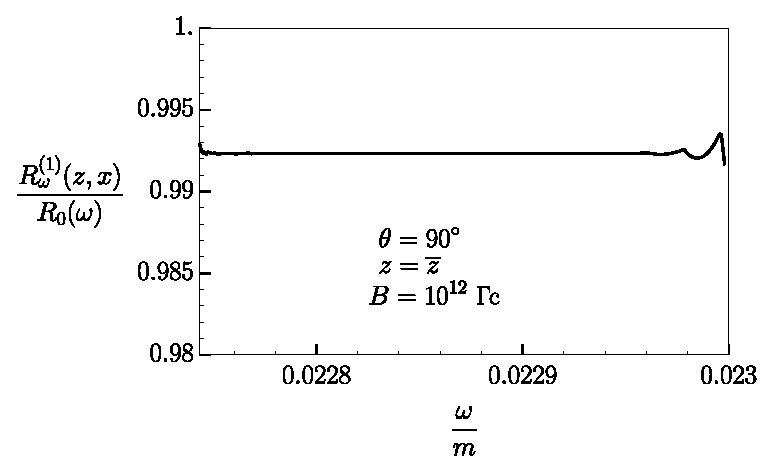
\includegraphics[width=1\linewidth,clip]{TransfMode1z24cmx90.eps}
	\caption{��������� ������������ ��������� ��������~(\ref{eq:PowerSpectra}) � ������������ ��������� �������� ������������� ���������~(\ref{eq:BlackPowerSpectra}) ��� ���� 1 ��� $z=24$ ��.}\label{fig:Transf1zkx24cm2}
\end{figure}

\begin{figure}\centering
	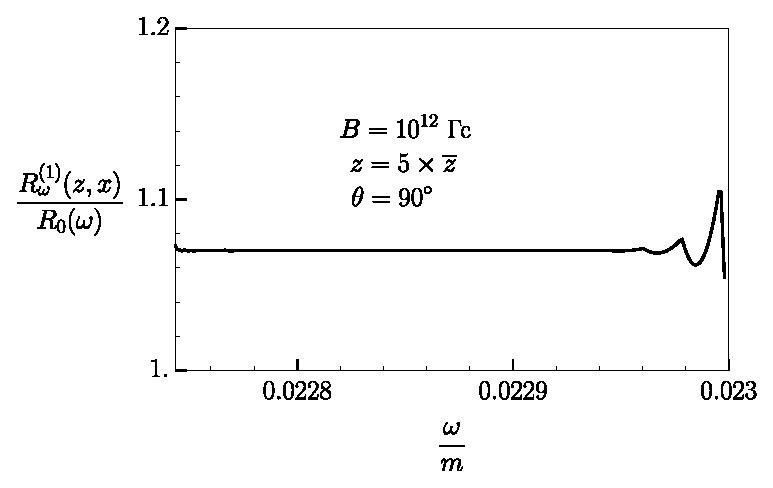
\includegraphics[width=1\linewidth,clip]{TransfMode1z120cmx90.eps}
	\caption{��������� ������������ ��������� ��������~(\ref{eq:PowerSpectra}) � ������������ ��������� �������� ������������� ���������~(\ref{eq:BlackPowerSpectra}) ��� ���� 1 ��� $z=120$ ��.}\label{fig:Transf1zkx120cm2}
\end{figure}

\begin{figure}\centering
	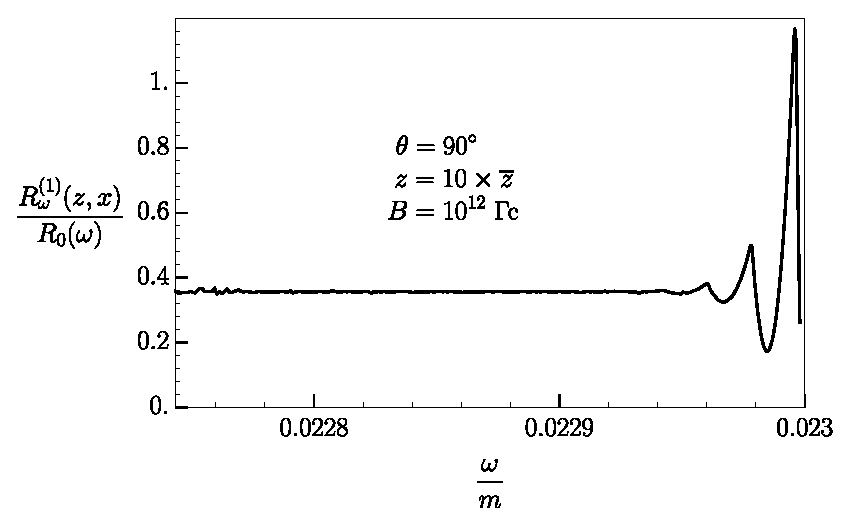
\includegraphics[width=1\linewidth,clip]{TransfMode1z240cmx90.eps}
	\caption{��������� ������������ ��������� ��������~(\ref{eq:PowerSpectra}) � ������������ ��������� �������� ������������� ���������~(\ref{eq:BlackPowerSpectra}) ��� ���� 1 ��� $z=240$ ��.}\label{fig:Transf1zkx240cm2}
\end{figure}
%%%%%%%%%%%%%%%%%%%%%%%%%%%%%%%%%%%%%%%%%%
%%%%%%%%%%%%%%%%%%%%%%%%%%%%%%%%%%%%%%%%%%
\begin{figure}\centering
	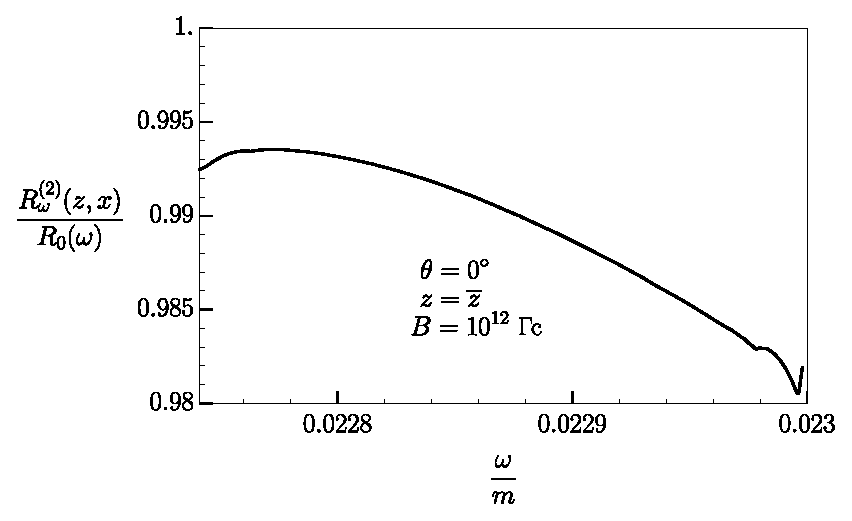
\includegraphics[width=1\linewidth,clip]{TransfMode2z24cmx0.eps}	\\
	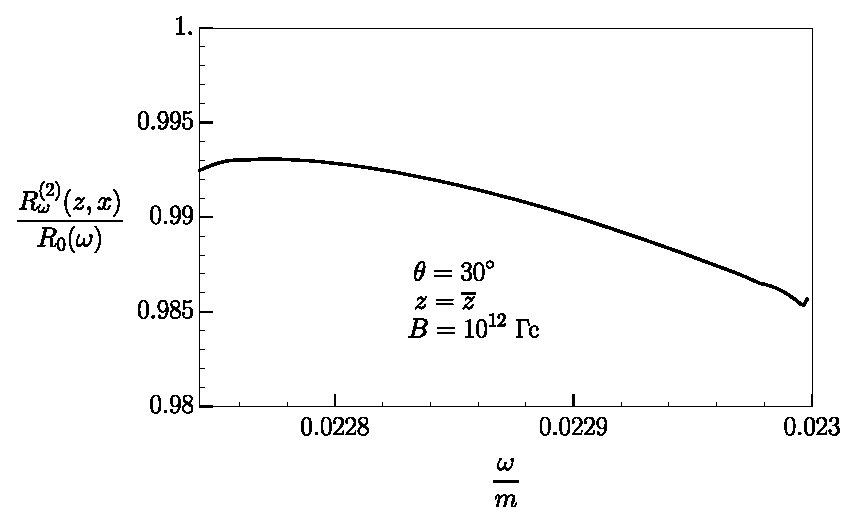
\includegraphics[width=1\linewidth,clip]{TransfMode2z24cmx30.eps}
	\caption{��������� ������������ ��������� ��������~(\ref{eq:PowerSpectra}) � ������������ ��������� �������� ������������� ���������~(\ref{eq:BlackPowerSpectra}) ��� ���� 2 ��� $z=24$ ��.}\label{fig:Transf2z24cm}
\end{figure}

\begin{figure}\centering
	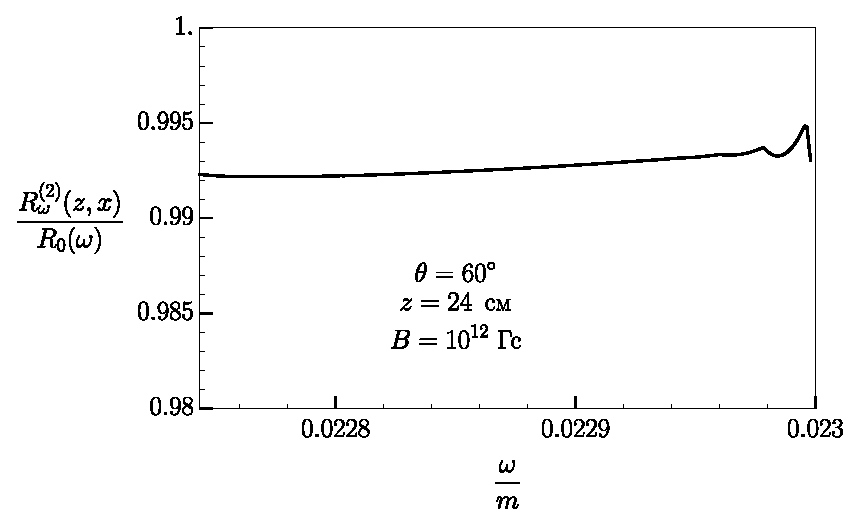
\includegraphics[width=1\linewidth,clip]{TransfMode2z24cmx60.eps}	\\
	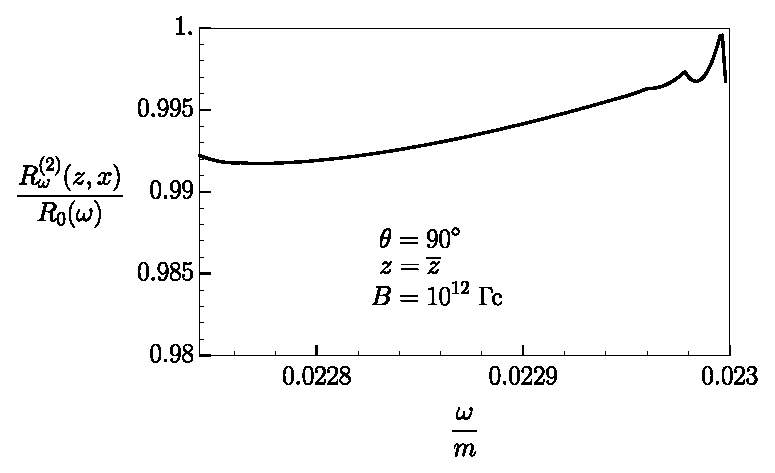
\includegraphics[width=1\linewidth,clip]{TransfMode2z24cmx90.eps}
	\caption{��������� ������������ ��������� ��������~(\ref{eq:PowerSpectra}) � ������������ ��������� �������� ������������� ���������~(\ref{eq:BlackPowerSpectra}) ��� ���� 2 ��� $z=24$ ��.}\label{fig:Transf2zkx24cm2}
\end{figure}

\begin{figure}\centering
	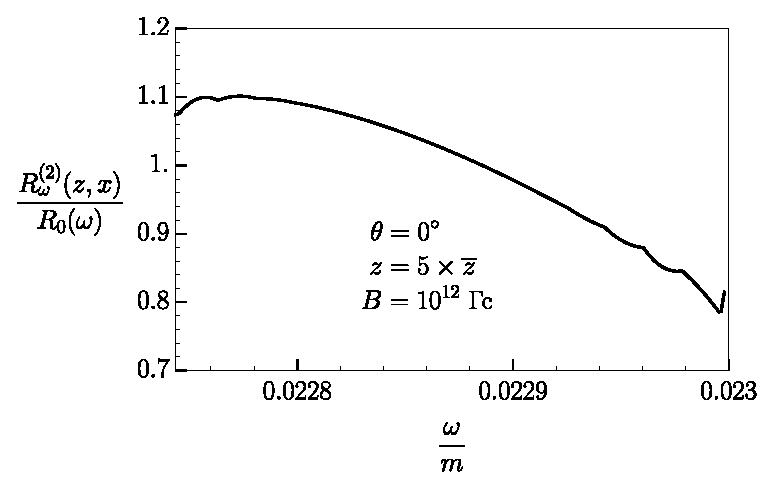
\includegraphics[width=1\linewidth,clip]{TransfMode2z120cmx0.eps}	\\
	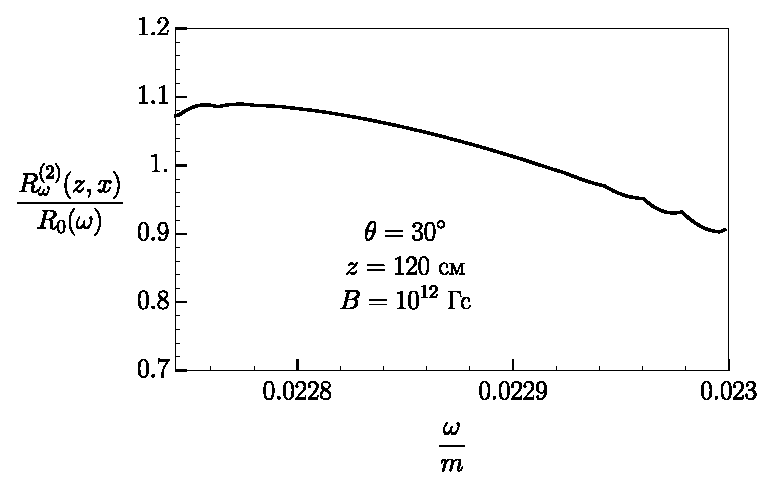
\includegraphics[width=1\linewidth,clip]{TransfMode2z120cmx30.eps}
	\caption{��������� ������������ ��������� ��������~(\ref{eq:PowerSpectra}) � ������������ ��������� �������� ������������� ���������~(\ref{eq:BlackPowerSpectra}) ��� ���� 2 ��� $z=120$ ��.}\label{fig:Transf2zkx120cm}
\end{figure}

\begin{figure}\centering
	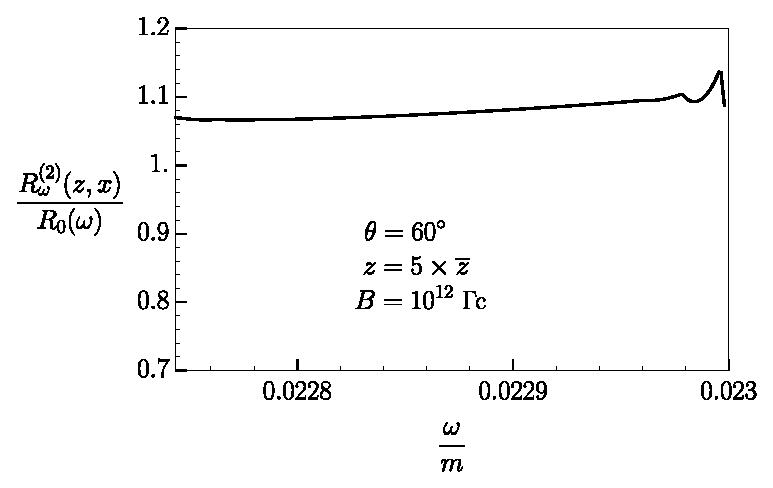
\includegraphics[width=1\linewidth,clip]{TransfMode2z120cmx60.eps}	\\
	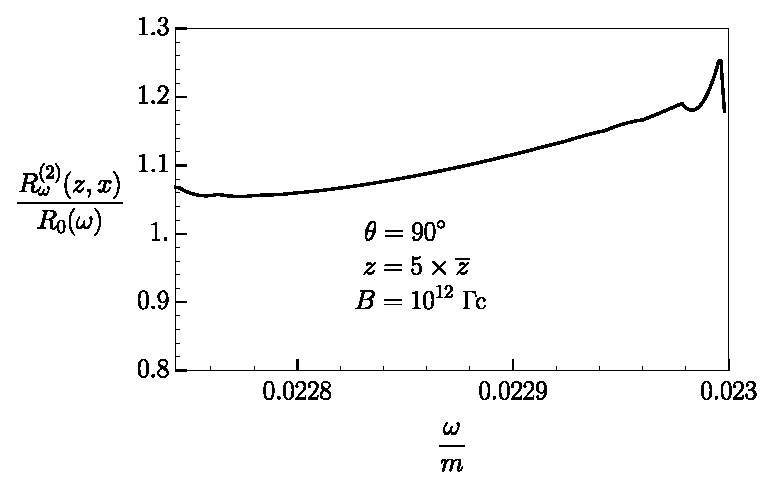
\includegraphics[width=1\linewidth,clip]{TransfMode2z120cmx90.eps}
	\caption{��������� ������������ ��������� ��������~(\ref{eq:PowerSpectra}) � ������������ ��������� �������� ������������� ���������~(\ref{eq:BlackPowerSpectra}) ��� ���� 2 ��� $z=120$ ��.}\label{fig:Transf2zkx120cm2}
\end{figure}

\begin{figure}\centering
	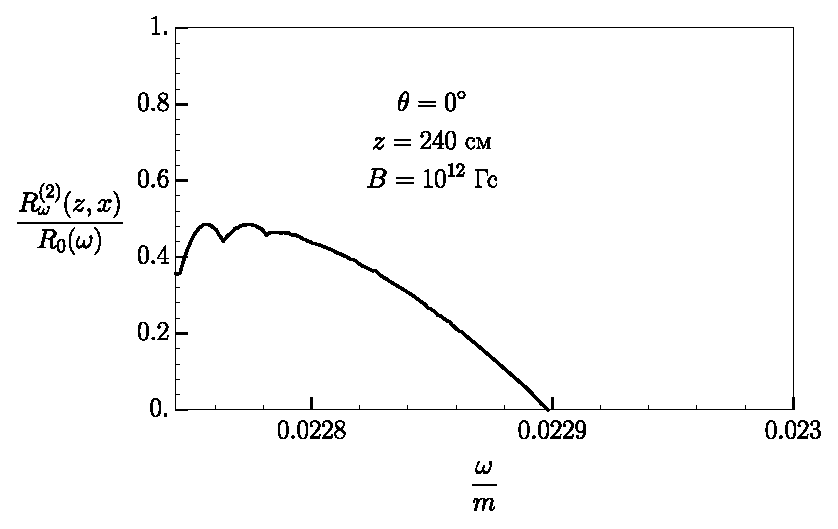
\includegraphics[width=1\linewidth,clip]{TransfMode2z240cmx0.eps}	\\
	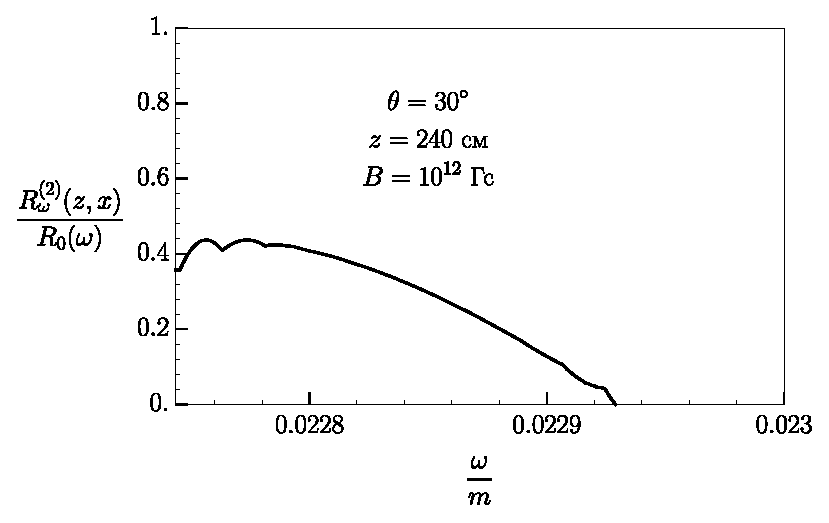
\includegraphics[width=1\linewidth,clip]{TransfMode2z240cmx30.eps}
	\caption{��������� ������������ ��������� ��������~(\ref{eq:PowerSpectra}) � ������������ ��������� �������� ������������� ���������~(\ref{eq:BlackPowerSpectra}) ��� ���� 2 ��� $z=240$ ��.}\label{fig:Transf2zkx240cm}
\end{figure}

\begin{figure}\centering
	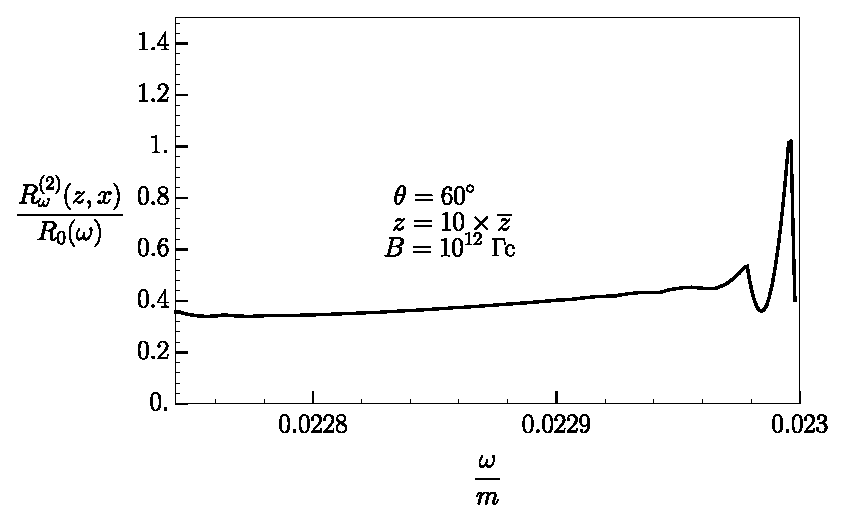
\includegraphics[width=1\linewidth,clip]{TransfMode2z240cmx60.eps}	\\
	\includegraphics[width=1\linewidth,clip]{TransfMode2z240cmx90.eps}
	\caption{��������� ������������ ��������� ��������~(\ref{eq:PowerSpectra}) � ������������ ��������� �������� ������������� ���������~(\ref{eq:BlackPowerSpectra}) ��� ���� 2 ��� $z=240$ ��.}\label{fig:Transf2zkx240cm2}
\end{figure}
\clearpage
\section{������}
����������� ������� ������������� ��������� ��� ���������� ������� ������������� ������� ���� ��������� ����������� � ����������� ���������������� $e^+e^-$ ������ � ������������ ������� ��������� ���� � ������ ��������� �� ����������� ���������.
�������������� �������������� ������� � ���������� ������� ������������� �� ��������� �������� ������ ������� � ������� ������� ���������������� ��������� �� ����������� ������������� ����� ����������. ������� ������������ � ���� ��������� �� ����������� ���������. ��� �������� ���������� ���� $B=10^{12}$ �� � $T\simeq11$ ��� ��������� ������������ ��������� ��������. ������� �������� ��������, ��� ��� ���� 1 � ����������� ������� ��� $z\lesssim 120$ �� ������ ����������� ��������� �� �������� ������� ����, � �� ����� ��� ��� ���� 2 ������������ ������������ ���������. ��� ����� �������� � ��� ��� ���� 1 ��� ����� �������� ����������� �� ������� �� ��������� ����������, ����� ��� ��������� ������ ���� 2 ����� �������� ����������� �������������. ������ ����� ����������� � ������������ ���������� ������������ (��., ��������,~\cite{Lubarsky:1988}). �� ������� ����������� ������� ������� �����������, ������� ����� ������� ������������ ������� �� ���������� ���� ��������������� �������. ���� ������ ������� �� ����� ��������� �����������.

���������� ���������� ����� ���� ������������ ��� ���������� ������� ��������� ������������ �������. ��� ����� ������� ��������� ������������ ������� �� ����� ������� (��., ��������, \cite{Nishimura:2008}) � ���������� ��������� ���������� ���� � �����������. �������������� ������ ����� ���� ������, ��� ����� ������� ���� ����� ��������. 
\documentclass[12pt]{article}

\usepackage{cite}
\usepackage{graphics}
\usepackage[cp866]{inputenc}
\usepackage[english,russian]{babel}
\usepackage{amssymb,graphicx}
\usepackage{doctor,my}

\setcounter{part}{3}
\setcounter{page}{104}
\setcounter{figure}{22}
\setcounter{table}{1}




% ��� ����� <~ = \lesssim �㦥�: amssymb.sty
%\documentstyle[12pt,russian,ourdef,amssymb]{article}


%  *** Useful macros ******

%************************************************

\begin{document}

\ruschapters

\ruschapt{�����祭��} 

\large
\setlength{\baselineskip}{24pt}

\inputencoding{cp866}


� �����饩 ������樨 ��᫥������ �⮭-����ਭ�� ������ � ������⢨� 
ᨫ쭮�� �����⭮�� ���� � ������.

� ������樨 �।�⠢���� ᫥���騥 १�����

\begin{enumerate}

\item 

���ᬮ�७, � ࠬ��� �⠭���⭮� ������, 
����� ����ਭ���� ஦����� ���⮭��� ���� ($\nu \to \nu \ell_1 \bar \ell_2$)
�� ���譥� �����஬����⭮� ����. 
����祭� �ࠢ��⥫쭮 ���⮥ ��ࠦ���� ��� ����⭮�� �����, 
�ࠢ������� �� �ந������� ���祭��� �������᪮�� ��ࠬ��� �  
㤮���� ��� �᫥����� �������. �஠������஢��� �������� ����䨧��᪨� 
�ਫ������ ��ᬮ�७���� �����.

\item

�஢���� ��騩 ������ �������� $n$-���設���� ������⫥���� 
 �����  
� ᨫ쭮� �����⭮� ���� � ��ᬮ�७� �⮭-����ਭ�� ������
$\gamma \gamma\to \nu \bar\nu $ (� ࠬ��� 
������ � ����襭��� ���� - �ࠢ�� ᨬ���ਥ�) 
� $\gamma \gamma \to \nu \bar\nu \gamma$ 
(� ࠬ��� �⠭���⭮� ������). 
��������, �� ࠧ���� ⨯� ��䥪⨢���� ����ਭ�-�����஭���� 
����������⢨� ����� � ࠧ���� ����ᨬ���� �������� �� 
����殮����� ����. � ��⭮��, �� ���⭮� �᫥ ���設 
� ��䥪⨢��� ᪠��୮� $\nu\nu e e$-�裡, ����� ������� 
� ���७�� �⠭���⭮� ������ � ����襭��� ����-�ࠢ�� 
ᨬ���ਥ�, ������㤠 �ᨫ������� ���譨� ������� �����, ⮣�� ���
��� �⭮�� �᫠ ���設 ⠪�� �ᨫ���� �������� ⮫쪮 � ��砥
��䥪⨢��� �ᥢ��᪠��୮�, ����୮� ��� ��ᨠ�쭮� �裡.   
��������, �� �� ⨯� ������� ����� ��ࠧ��� �१ ��������� �㭪樨.   
����祭� ��騥 ��ࠦ���� ��� ������� ����ᮢ 
$\gamma \gamma\to \nu \bar\nu $ � $\gamma \gamma \to \nu \bar\nu \gamma$,
�ࠢ������ �� �ந������� ���ࣨ�� �⮭��.
� �।��쭮� ��砥 ������ ���ࣨ� �⮭�� ���᫥�� �祭�� 
����� $\gamma \gamma \to \nu \bar\nu \gamma$. 
����祭� �業�� ��� ����ਭ��� ᢥ⨬��� �⮭���� ���� � �।��� 
����� � ������ ⥬������. ��������, ��,  
 � ����ᨬ��� 
�� ⥬������� � ����稭� �����⭮�� ����, ������ � ����ਭ��� ᢥ⨬���� 
�� ��� ��ᬠ�ਢ����� ����ᮢ 
����� ��� ������஢���, ⠪ � ��������� ���������묨 �� 
�ࠢ����� � ������� ����� 
$\gamma \gamma\to \nu \bar\nu $, ����祭�� � ࠬ��� �⠭���⭮� ������. 

\item

���᫥�� ������㤠 ����� ��饯����� 
�⮭� $\gamma \to \gamma \gamma$ � ᨫ쭮 �������祭��� ������, 
�஠������஢��� ���  ������⨪� � ������� �ࠢ��� �⡮� �� ����ਧ���. 
 ��� ࠧ�襭��� ������� ��饯����� ���᫥�� ᮮ⢥�����騥 
����⭮�� � ��⮬ ��ᯥ�ᨨ � ��७�ନ஢�� �������� 
�㭪権 �⮭��. 
����祭�� १����� �����뢠��, �� ������⢨� ������, � ����� 
��஭�, ����⢥��� ��ࠧ�� ������� �ࠢ��� �⡮� �� ����ਧ��� 
�� �ࠢ����� � ��砥� ��⮣� �����⭮�� ����.
� ��⭮��, �⠭������ �������� ���� ����� ��饯����� 
$\gamma_2 \to \gamma_1 \gamma_1$, ����饭�� � ������⢨� ������.
� ��㣮� ��஭�, ������ ������ 
����뢠�� ��������饥 ���ﭨ� �� ������ $\gamma_1 \to \gamma_1 \gamma_2$ 
� $\gamma_1 \to \gamma_2 \gamma_2$. ��� �� �����, 
宫����� ���冷��-ᨬ����筠� ������ � ��⠭�� � ᨫ�� 
������� ����� ᯮᮡ�� �ᨫ��� ����⭮��� ��饯����� �� �⨬ ������� 
�� �ࠢ����� � ���� ������� �����. 


\end{enumerate}

�᭮��� १����� ������樨 ��㡫������� � ࠡ���   
\cite{Kuznetsov:2000mp,Kuznetsov:2002it,Kuznetsov:2001sb,Kuznetsov:2003sb,
Kuznetsov:2004a,Kuznetsov:2004sb,Kuznetsov:2002a,Kuznetsov:2002q,Rumyantsev:2004sb}

\bigskip

���� ��ࠦ��� ��㡮��� �������୮��� ���筮�� �㪮����⥫� 
����ᠭ��� ��ᨫ쥢��� �㧭�殢� �� ����ﭭ�� �������� � ࠡ��, 
���㦤���� ����祭��� १���⮢, ᮢ��� � ������, �������� ��� �� 
�믮������ ������樨. ����� ���⭮ ������������ �.�. ��奥��, 
�.�. ����类��, �.�. ��������, �.�. ���宬����, �.�. ������� � 
�.�. ������ �� �����প�. 
���� ��������� ⠪�� ���. �.�. �㡠���� �� ������� ���㦤����. 

\newpage
\input ref.tex

\end{document}


\appendix
\newpage
\chapter{������ ���������� �������� � ��������� ����}\label{appA:AccurProp}
��� ������������ ������ �������������� � ��������� ������ ���� ��������������, ��� ����� ���������� � ��������� ����������� ���������� ����� ������������ ���������. "�������������" ������� ��������, ��� �� ������� � ������� �� ������� �������������� ������������~(\ref{eq:Energy_n}). ������������� ��������� � ���������� ������������ ������� ����~\cite{Schwinger:1951} ����������� ���������� ������ � $\delta$-�������� � ������ �����:
%
\begin{equation}\label{eq:Green}
	(\ii\partial_\mu \gamma^\mu + e_f A_\mu \gamma^\mu - m_f) S(X,X')=\delta\left(X-X'\right)\, .
\end{equation}
%

��� ������� $S(X,X')$ ���������� ������������. � ���� ������� �� ������ ������������� ������������ ��������� �� ������� ��������� ���� � ������ ������������ �������� � ��������� ��������� � �������, ��� ����� ��������������� �������� � ��������� ���������, ���������� �������� � ������������� ���������.

������� ���������~(\ref{eq:Green}) ����� ���������� ���������� ���. ������� ������ ��������������� ���������� �������������. � ������������ ������� ����� ��� ������, ���������� ������� �������� �������, $|e_f|/m_f$, ������ ������������� ���������� � ���� ���������� �� ������� ������:
\begin{equation}
	S(X,X') = \sum_{n=0}^{\infty}\sum_{s=\pm 1} S_n^s (X,X')\, .
\end{equation}

��� ���������� ����������� ����� ��������������� �������� �����������:
%
\begin{eqnarray}
	\Psi (X) = \sum\limits_{n,p_y,p_z,s} ( a^{s}_{n,p} \Psi_{n,p,+}^s (X) + b^{\dagger s}_{n,p} \Psi_{n,p,-}^s (X) )\,,
\end{eqnarray}
\noindent ��� $a$ -- �������� ����������� ��������, $b^{\dagger}$ -- �������� �������� ��������, $\Psi_{+}$ � $\Psi_{-}$ ������������� �������� ��������� ������ � ������������� � ������������� �������� ��������������. ����������� ������� ���������� ����������� ��� �������� �������������� �������������� � ��������� �������������� ������������ ������� ����������:%~\cite{Fock1937}
%
\begin{equation}
	S(X,X') = T(\Psi(X)\bar{\Psi}(X')) - {\cal N}(\Psi(X)\bar{\Psi}(X'))\, .
\end{equation}
%

���������� ������ ������� ��������� ������~(\ref{eq:psie}) � ����� ��� �������� ����� �����������:
\begin{eqnarray}
	\phi^{s}_{p, n} (X_1) =   \frac{U^s_{n} [\xi(X_1)]}
	{\sqrt{2 M_n (E_{n} + M_n)(M_n + m_f)}} \, ,
	\label{eq:phi_psi}
\end{eqnarray}
%
\noindent ��� $U^s_{n}$ ������������ ��������~(\ref{eq:U^s}), ����� ����������� ����� � ���������� ����������� �� ������ ������ $n$ � ���������������� ��������� $s$ ��������� �������:
\begin{eqnarray}
	\label{eq:propagator}
	S^{s}_n (X, X^{\,\prime}) && =  \int \frac{\dd p_0 \dd p_y \dd p_z}{(2\pi)^3} \times
	\\[3mm]
	\nonumber
	&& \times \frac{\eee^{- \, \ii \,  p_0 \,(X_0 - X^{\,\prime}_0) + 
			\ii p_y \,(X_2 - X^{\,\prime}_2) +  \ii \,  p_z \,(X_3 - X^{\,\prime}_3)}}
	{p_0^2 - p_z^2 - M_n^2 - {\cal R}^{s}_\Sigma (p) + \ii\, {\cal I}^{s}_\Sigma (p)}
	\, \phi^{s}_{p, n} (X_1) \bar \phi^{s}_{p, n} (X'_1) \, ,
\end{eqnarray}
��� ${\cal R}^{s}_\Sigma (p)$ � ${\cal I}^{s}_\Sigma (p)$ -- �������� � ������ ����� ��������� ��������� ��������.  ��� �� ��������� ��������� ��������� ������������ �������� � ����� �������� � ������������� ������. �������� ����� ��������� ��������� ${\cal R}^{s}_\Sigma (p)$ ���������� ��������� ������ ��������� �������� � ����������� ������������� ������. � ������ ��������� �����, ��� ����������� $B\ll B_e$, �� ����� ��� ����� ������������� ��� ����������������, ��� ������������ 
����������~\cite{Ritus1969}:
%
\begin{eqnarray}
	\label{eq:Re1}
	\Re^{s}_\Sigma (p) = \frac{4\alpha m_f}{3\pi} \varkappa^2 \left [ \ln \varkappa^{-1} + C + \frac{1}{2} \ln 3 - \frac{33}{16} \right],\quad \varkappa\ll 1,
\end{eqnarray}
\noindent ��� $C = 0.577...$ - ���������� ������, ������������ �������� $\varkappa$ �������� ��������� �������:
%
\begin{eqnarray}
	\varkappa = \frac{1}{m_f B_e} [-(F_{\mu\nu} p_{\nu})^2]^{1/2}.
\end{eqnarray}
%

��� ������ �������� ���������� ����, $B\gtrsim B_e$, ��� ����� ������ ���������� ����� �  ����� ����� ��������, ������������ �� �������� ������ ������, ����������� ��������� ��������������� �������~\cite{Jancovici:1969}:
\begin{eqnarray}
	\label{eq:Re2}
	\Re^{s}_\Sigma (p) = \frac{\alpha}{4\pi} m_f \ln^2 (2\beta/m_f^2).
\end{eqnarray}
%

�� (\ref{eq:Re1}) � (\ref{eq:Re2}) �������, ��� ���� ��� ���������� ������� �������� ���������� ���� ������ �� $10^{16}$ �� ��� �������� � ����� �������� ����� �������� ������� ���������� ������ ��������� $\alpha$~\cite{Kuznetsov:2003,Sokolov:1986} � �������� ��������������.

�������� �� ����������� �������� ����� �����������, ����� � ����������� �����������~(\ref{eq:propagator}) �������� ����� ���������� � ����. ����� ����������� ������� ���������� ��������, �� ���� ����������� ������������ ����� ���������~(\ref{eq:Energy_n}). ������ ���������� ����������, ��� ��� �������� ������ �����, ����� ����������� ������� �������� ���� �� ������ ������� ������, $n > 0$. ������� ��� ���� �������� ������������, � ����� �� �����, � ������������� ������� ���������������� ���������� �������, ������������ ������ ������ ��������� ���������,  ${\cal I}^{s}_\Sigma (p)$, ���� ������� ���������� �����������. ��� ����� ���� �������� � ������� ���������� ������� � ������������ � ��������� ����~\cite{Borisov:1997, Zhukovski:1994}:
%
\begin{eqnarray}
	\Im^{s}_\Sigma (p) = - \frac{1}{2}\, p_0 \; \Gamma_n^{s} \, ,
	\label{eq:I_Sigma}
\end{eqnarray}
\noindent ��� $\Gamma_n^{s}$ -- ������ ������ ���������� ��������, ������������ � ��������������� ��������� $s$ � �����������  $n$-� ������� ������. ������ ������ ��������� ��������� �������� ����� ���� �������� ����� 
������ �������� ��������~\cite{Weldon:1983}:
%
\begin{eqnarray}
	\label{Gns}
	\Gamma_n^{s} = \Gamma^{(abs)\, s}_n + \Gamma^{(cr) \, s}_n \simeq 
	\Gamma^{(cr) \, s}_{n} 
	\left [1+ \eee^{(E_n - \mu)/T} \right ]\, ,
\end{eqnarray}
��� $\Gamma^{(abs)\, s}_n$ � $\Gamma^{(cr) \, s}_n$ -- ������ ���������� � �������� �������� ��������������. ��������� ����� ������� ���������� � ������ �������� ������ ��������� ��������� ��������  ��������� ��������� ������������ ������� ��������� ��������� � ����������� �������. 
\chapter{���������� ��� ${\cal T}^{s'' s}_{k}$}

\label{Sec:app_c}

������� ${\cal T}^{s'' s}_{k}$, �������� �~(\ref{eq:amplonever}), ��������� ��� ������ �������������� 
������ ��������, $\eta = -1$, �  ����� ���� �������� 
� �������������� �������� �������~(\ref{eq:psie}). 
������������ ��������� �����������:  ${\cal I}_{n, \ell} \equiv {\cal I}_{n, \ell}
\left ({q^{2}_{\mprp}}/{(2 \beta)} \right )$.

%��� �������������� ������ ��������, $\eta = -1$ �������  ${\cal T}^{s'' s}_{k}$, �������� �~(\ref{eq:amplonever}), ����� ���� �������� 
%� �������������� �������� �������~(\ref{eq:psie})  
%� ������������ � ��������� ������-������������ �����: 

{\bf 1.} � ������, �����  $j$  �������� ���������� ����� 
($k = S$), ���������� ���� 


\begin{eqnarray}
{\cal T}^{--}_S = g_S j_S {\cal K}_3 [ (m_f+M_\ell)(m_f+M_n)  {\cal I}_{n,\ell} - 
2\beta \sqrt{\ell n} {\cal I}_{n-1,\ell-1} ] \, ;
\end{eqnarray}
%
\begin{eqnarray}
{\cal T}^{-+}_S = -\ii g_S j_S {\cal K}_4 [\sqrt{2\beta n} (m_f+M_\ell) 
{\cal I}_{n-1,\ell-1} + 
\sqrt{2\beta \ell} (m_f+M_n)  {\cal I}_{n,\ell} ] \, ;
\end{eqnarray}
%
\begin{eqnarray}
{\cal T}^{+-}_S = -\ii g_S j_S {\cal K}_4 [\sqrt{2\beta \ell} (m_f+M_n) 
{\cal I}_{n-1,\ell-1} + 
\sqrt{2\beta n} (m_f+M_\ell)  {\cal I}_{n,\ell} ] \, ;
\end{eqnarray}
%
\begin{eqnarray}
{\cal T}^{++}_S = g_S j_S {\cal K}_3 [(m_f+M_\ell)(m_f+M_n)  {\cal I}_{n-1,\ell-1} -
2\beta \sqrt{\ell n} {\cal I}_{n,\ell} ] \, .
\end{eqnarray}

{\bf 2.} � ������, �����  $j$  �������� ���������������� ����� 
($k = P$), �������


\begin{eqnarray}
{\cal T}^{--}_P =  g_P j_P {\cal K}_4 [ 2\beta\sqrt{\ell n}  {\cal I}_{n-1,\ell-1} +
(m_f+M_\ell)(m_f+M_n) {\cal I}_{n,\ell} ] \, ;
\end{eqnarray}
%
\begin{eqnarray}
{\cal T}^{-+}_P =  \ii g_P j_P {\cal K}_3 [ \sqrt{2\beta n} (m_f+M_\ell) 
{\cal I}_{n-1,\ell-1} - 
\sqrt{2\beta \ell} (m_f+M_n)  {\cal I}_{n,\ell} ] \, ;
\end{eqnarray}
%
\begin{eqnarray}
{\cal T}^{+-}_P =  \ii g_P j_P {\cal K}_3 [\sqrt{2\beta \ell} (m_f+M_n) 
{\cal I}_{n-1,\ell-1} - 
\sqrt{2\beta n} (m_f+M_\ell)  {\cal I}_{n,\ell} ] \, ;
\end{eqnarray}
%
\begin{eqnarray}
{\cal T}^{++}_P = - g_P j_P {\cal K}_4 [(m_f+M_\ell)(m_f+M_n)  {\cal I}_{n-1,\ell-1} +
2\beta\sqrt{\ell n} {\cal I}_{n,\ell} ] \, .
\end{eqnarray}

\newpage

{\bf 3.} � ������, �����  $j$  �������� ���������  ����� 
($k = V$), ����� �����


\begin{eqnarray}
\nonumber
&&{\cal T}^{--}_V  = g_V [ 2\beta\sqrt{\ell n} ({\cal K}_1 j_V) {\cal I}_{n-1,\ell-1} +
(m_f+M_\ell)(m_f+M_n) ({\cal K}_1 j_V) {\cal I}_{n,\ell} -
\\[3mm]
\label{eq:tV--}
%transversal
&&-\sqrt{2\beta n} (m_f+M_\ell) {\cal K}_3 \frac{(j_V\Lambda q) - 
	\ii (j_V \varphi q)}{\sqrt{q^2_{\mprp}}} {\cal I}_{n-1,\ell} -
\\[3mm]
\nonumber
&& - \sqrt{2\beta \ell} (m_f+M_n) {\cal K}_3 
\frac{(j_V\Lambda q) + \ii (j_V\varphi q)}{\sqrt{q^2_{\mprp}}} {\cal I}_{n,\ell-1}] \, ;
\end{eqnarray}
%
\begin{eqnarray}
\nonumber
&&{\cal T}^{-+}_V = \ii g_V [\sqrt{2\beta n} (m_f+M_\ell) ({\cal K}_2 j_V) 
{\cal I}_{n-1,\ell-1} - 
\sqrt{2\beta \ell} (m_f+M_n) ({\cal K}_2 j_V) 
{\cal I}_{n,l} +
\\[3mm]
\label{eq:tV-+}
%transversal
&&+ 2\beta\sqrt{\ell n} {\cal K}_4 
\frac{(j_V\Lambda q) - \ii (j_V \varphi q)}{\sqrt{q^2_{\mprp}}} {\cal I}_{n-1,\ell} -
\\[3mm]
\nonumber
&&- (m_f+M_\ell)(m_f+M_n) {\cal K}_4 
\frac{(j_V\Lambda q) + \ii (j_V\varphi q)}{\sqrt{q^2_{\mprp}}} {\cal I}_{n,\ell-1}]  \, ;
\end{eqnarray}
%
\begin{eqnarray}
\nonumber
&&{\cal T}^{+-}_V = -\ii g_V [\sqrt{2\beta \ell} (m_f+M_n) ({\cal K}_2 j_V) 
{\cal I}_{n-1,\ell-1} - 
\sqrt{2\beta n} (m_f+M_\ell) ({\cal K}_2 j_V) 
{\cal I}_{n,\ell} +
\\[3mm]
\label{eq:tV+-}
%transversal
&&+ (m_f+M_\ell)(m_f+M_n) {\cal K}_4 
\frac{(j_V\Lambda q) - \ii (j_V \varphi q)}{\sqrt{q^2_{\mprp}}} {\cal I}_{n-1,\ell} -
\\[3mm]
\nonumber
&&- 2\beta\sqrt{\ell n} {\cal K}_4 
\frac{(j_V\Lambda q) + \ii (j_V \varphi q)}{\sqrt{q^2_{\mprp}}} {\cal I}_{n,\ell-1}]  \, ;
\end{eqnarray}
%
\begin{eqnarray}
\nonumber
&&{\cal T}^{++}_V  = g_V [2\beta\sqrt{\ell n} ({\cal K}_1 j_V) {\cal I}_{n,\ell} +
(m_f+M_\ell)(m_f+M_n) ({\cal K}_1 j_V) {\cal I}_{n-1,\ell-1} -
\\[3mm]
\label{eq:tV++} 
%transversal
&&- \sqrt{2\beta \ell} (m_f+M_n) {\cal K}_3 
\frac{(j_V\Lambda q) - \ii (j_V\varphi q)}{\sqrt{q^2_{\mprp}}} {\cal I}_{n-1,\ell} -
\\[3mm]
\nonumber
&&- \sqrt{2\beta n} (m_f+M_\ell) {\cal K}_3 
\frac{(j_V\Lambda q) + \ii (j_V \varphi q)}{\sqrt{q^2_{\mprp}}} {\cal I}_{n,\ell-1}] \, .
\end{eqnarray}

\newpage

{\bf 4.} � ������, �����  $j$  �������� ��������������� ����� 
($k = A$), ������� 


\begin{eqnarray}
\nonumber
&&{\cal T}^{--}_A  = - g_A [2\beta\sqrt{\ell n} ({\cal K}_2 j_A) {\cal I}_{n-1,\ell-1} -
(m_f+M_\ell)(m_f+M_n) ({\cal K}_2 j_A) {\cal I}_{n,\ell} + 
\\[3mm]
\label{eq:tA--} 
%transversal
&&+ \sqrt{2\beta n} (m_f+M_\ell) {\cal K}_4 
\frac{(j_A\Lambda q) - \ii (j_A\varphi q)}{\sqrt{q^2_{\mprp}}} {\cal I}_{n-1,\ell} -
\\[3mm]
\nonumber
&&- \sqrt{2\beta \ell} (m_f+M_n) {\cal K}_4
\frac{(j_A\Lambda q) + \ii (j_A\varphi q)}{\sqrt{q^2_{\mprp}}} {\cal I}_{n,\ell-1}] \, ;
\end{eqnarray}
%
\begin{eqnarray}
\nonumber
&&{\cal T}^{-+}_A  =  \ii g_A [\sqrt{2\beta n} (m_f+M_\ell) ({\cal K}_1 j_A)
{\cal I}_{n-1,\ell-1} + 
\sqrt{2\beta \ell} (m_f+M_n) ({\cal K}_1 j_A) {\cal I}_{n,\ell} -
\\[3mm]
\label{eq:tA-+} 
%transversal
&&- 2\beta\sqrt{\ell n} {\cal K}_3
\frac{(j_A\Lambda q) - \ii (j_A\varphi q)}{\sqrt{q^2_{\mprp}}} {\cal I}_{n-1,\ell} - 
\\[3mm]
\nonumber
&&- (m_f+M_\ell)(m_f+M_n) {\cal K}_3
\frac{(j_A\Lambda q) + \ii (j_A\varphi q)}{\sqrt{q^2_{\mprp}}} {\cal I}_{n,\ell-1}] \, ;
\end{eqnarray}
%
\begin{eqnarray}
\nonumber
&&{\cal T}^{+-}_A  = -\ii g_A [\sqrt{2\beta \ell} (m_f+M_n) ({\cal K}_1 j_A)
{\cal I}_{n-1,\ell-1} + 
\sqrt{2\beta n} (m_f+M_\ell) ({\cal K}_1 j_A) {\cal I}_{n,\ell} -
\\[3mm]
\label{eq:tA+-} 
%transversal
&&- 2\beta\sqrt{\ell n} {\cal K}_3
\frac{(j_A\Lambda q + \ii (j_A\varphi q)}{\sqrt{q^2_{\mprp}}} {\cal I}_{n,\ell-1} - 
\\[3mm]
\nonumber
&&- (m_f+M_\ell)(m_f+M_n) {\cal K}_3
\frac{(j_A\Lambda q) - \ii (j_A\varphi q)}{\sqrt{q^2_{\mprp}}} {\cal I}_{n-1,\ell}] \, ;
\end{eqnarray}
%
\begin{eqnarray}
\nonumber
&&{\cal T}^{++}_A  = - g_A [(m_f+M_\ell)(m_f+M_n) ({\cal K}_2 j_A) {\cal I}_{n-1,\ell-1} -
2\beta\sqrt{\ell n} ({\cal K}_2 j_A) {\cal I}_{n,\ell} + 
\\[3mm]
\label{eq:tA++} 
%transversal
&&+ \sqrt{2\beta \ell} (m_f+M_n) {\cal K}_4 
\frac{(j_A\Lambda q) - \ii (j_A\varphi q)}{\sqrt{q^2_{\mprp}}} {\cal I}_{n-1,\ell} -
\\[3mm]
\nonumber
&&- \sqrt{2\beta n} (m_f+M_\ell) {\cal K}_4
\frac{(j_A\Lambda q) + \ii (j_A\varphi q)}{\sqrt{q^2_{\mprp}}} {\cal I}_{n,\ell-1}] \, .
\end{eqnarray}


�������, ��� ���������� ��������� ��� ��������� � ���������-��������� ������, 
����� ���������� � ������� � ������������ �� ��������������� ���������� ���������,  
����������� � ����� ����������� ������������ �  �������~\cite{Latal:86,Kaminker:1992a,Kaminker:1992b}.



\newpage

\chapter{��������������� � ������������� �������� ������} 
\label{app3}
��������������� � ������������� �������� ������ ������������ ��������������� ���������� ������ ${\cal P}_{\alpha\beta}$, ����� ��� �������� ����� ���� ������� �� ����������� �����~\cite{Shabad:1988,Tsai:1974,Batalin:1971,Skobelev:1975}. ��� ������� ������� ���������������� ��������� ������ ��������� ${\cal P}_{\alpha\beta}$ �� ������ �� 4-��������~\cite{Batalin:1971}, ������������ �� ������� ����������������� ���� � 4-������� �������� ������~$q_\alpha$:
\begin{equation}
	\begin{gathered}
	\label{eq:basis}
	b_{\mu}^{(1)} = (\varphi q)_\mu, \qquad
	b_{\mu}^{(2)} = (\tilde \varphi q)_\mu, 
	\\
	b_{\mu}^{(3)} = q^2 \, (\Lambda q)_\mu - q_\mu \, q^2_{\mbox{\tiny $\bot$}}, 
	\qquad b_{\mu}^{(4)} = q_\mu, 
	\end{gathered}
\end{equation}

\noindent ���������� ������������ ��������� ���������������� ��������� � ���������� 
���������� ��������� ����. ��� ���� $(b^{(1)} b^{*(1)}) = -q^2_{\mprp}$, 
$(b^{(2)} b^{*(2)}) = -q^2_{\mprl}$, $(b^{(3)} b^{*(3)}) = -q^2 q^2_{\mprl} 
q^2_{\mprp}$, $(b^{(4)} b^{*(4)}) = q^2$.  


� ������������� ������ ${\cal P}_{\alpha \beta}$ ��� �� ����� ������������ � ������ �� ��������~(\ref{eq:basis}), ������� ��� ������ ���������  �� ����������� �������� 
$r_{\alpha}^{(\lambda)}$ � ������������� ������ � ���������������� ������������ 
���������� ${\cal P}^{(\lambda)}$~\cite{Rojas1979r,Rojas1982,Shabad:1988,MRCh:2014}:
%
\beq
\label{eq:Pab10}
{\cal P}_{\alpha \beta} = \sum_{\lambda = 1}^{3} 
{\cal P}^{(\lambda)} \, \frac{r_{\alpha}^{(\lambda)} 
	(r_{\beta}^{(\lambda)})^{*}}{(r^{(\lambda)})^2} \, , \quad 
r_{\beta}^{(\lambda)} = \sum\limits_{i = 1}^{3} A_i^{(\lambda)} \, b_{\beta}^{(i)} \, , 
\eeq
\noindent ���  $A_i^{(\lambda)}$ ��������� ����������� ������������.


��� ������������ ��������� ������� � ������ ������������� 
������, ���������� ��� �����  ����� ���������� ����  �� ��������� $u_{\alpha}$,  
����� ����������� �������� ������  ���������� ���� ��� ������������� ������������. � ���� ������ ����������� 
������� ������������� ���������� � ���������� ������, ������� ����������� $T$ � ���������� ���������  $\mu$ 
����� ���� ��������  � ����� ������-������������ ����: 

%����� ���������� ������� ��������� ���������. ��������� � ������� �� ����������, ��� �������������� ���� �������� 
%${\cal E}_e = B_e$ �������� ����������,  
%�� ��������� � ���������������� ������� ������������ �������������� ���� 
%������� ������������ �������� � ������������ �������� �������� - ����������� 
%��� �� �������. � ������ �������, � ������������ ��� ������������� ���� ���������� 
%��������������� ���������� ������������� ���� ${\cal E}$ ����� ��������� 
%����������� �������� $B_e$, ��������� ��� ���� ������ $B$. 
%�� � ���� ������ ��������������� ������� ������ ����� ������� 
%� ������� �������, ��� ���� ������ ��������� ����. ��� ����������� ����� �������� � �� 
% ������, ����� ������, ������� ����������� $T$ � ���������� ���������  $\mu$
%��������, ��� �����, ����� ���������� ����. 
%��� ����� ����������  �������  ������������� ����������  �������� � ����� ������-������������ 
%����, ����� 4-������ �������� �����, $u_\alpha$:
%
\beq
\label{eq:fermidist}
&&f_{\pm}(p) = \frac{1}{1+\exp{[((pu)_{\mprl} \pm \mu)/T]}} \, , 
\\ [3mm]
\nonumber
&&(pu)_{\mprl} = E u_0 - p_z u_z \, , \quad E=\sqrt{p_z^2+m^2} \, .
\eeq
\noindent ����� ������� ���� ������������� �����������, � ������ -- ����������� ����������� ������.

%��� ���� �������, ��� � ����� ������� �����������  
%������������� ����, ����� ���� �������� � 
%�������������-������������ ����: $(u \Lambda)_\mu = 0$. 
% �������������, � ������, ����� ������ �������� ��� ����� ����� ���������� ����  �� 
%��������� $u_{\alpha}$,  
%����� ����������� �������� ������ ������� ���������� ����. 
� ������ ����� ���������, � ������ ������ ������������� ������, ����� ��������� ���� �������� 
����������  ���������� ������,
$\beta \gg m^2,\, \mu^2, \, T^2$, ��������� 
���������� �����~\cite{Rojas1979,Rojas1982,Rojas1979r,Shabad:1988} 
��� ${\cal P}_{\alpha \beta}$, ����� �������� ��������� ���������� �� 
�������� �������� ���������� ����:
%
\beq
\label{eq:Pab1}
&&{\cal P}_{\alpha \beta} = \sum_{\lambda} 
{\cal P}^{(\lambda)} \, \frac{r_{\alpha}^{(\lambda)} (r_{\beta}^{(\lambda)})^{*}}{(r^{(\lambda)})^2} 
\simeq 
- \frac{2\alpha}{\pi} \; \beta \, {\cal D} \, 
\frac{(\tilde \varphi q)_\alpha (\tilde \varphi q)_\beta}{q^2_{\mprl}} 
+ 
\\
\nonumber
&&+\frac{\alpha}{3\pi}\; (\varphi q)_\alpha (\varphi q)_\beta 
+\frac{\ii \alpha}{\pi} \, \Delta N \, \left [
\varphi_{\alpha \beta} \, (qu) + (q\varphi)_{\alpha} u_{\beta} - 
(q\varphi)_{\beta} u_{\alpha} \right ]  +
\\
\nonumber
&& + \frac{\alpha}{3\pi} \, {\cal V} \, \left (q^2 \, g_{\alpha \beta} - 
q_{\alpha} \, q_{\beta} \right )  + 
O \left (\frac{1}{\beta} \right) \, , 
\eeq  
\noindent ��� 
%
\beq
\label{eq:PabD}
{\cal D} = - {\cal J}_1 (q_{\mprl})  - 
H \left (\frac{q^2_{\mprl}}{4m^2} \right)  \, , 
\eeq
%
\beq
\label{eq:PabJ}
{\cal J}_1 (q_{\mprl}) = 2q^2_{\mprl} \, m^2 \, \int\limits_{-\infty}^{\infty}  \frac{\dd p_z}{E} \, 
\frac{f_{-}(p) + f_{+}(p)}{q_{\mprl}^4 - 4(pq)^2_{\mprl}} \, , 
\eeq
%
\beq
\label{eq:H0}
%\nonumber
H(z)&=&\frac{1}{\sqrt{z(1 - z)}} \, \arctg \sqrt{\frac{z}{1 - z}} - 1,
\quad 0 \leqslant z \leqslant 1,
\\ [3mm]
\label{eq:H1}
H(z) &=& - \frac{1}{2\sqrt{z(z-1)}}
\ln  \frac{\sqrt{z} + \sqrt{z-1}}{\sqrt{z} - \sqrt{z-1}}  - 1 + 
\\[3mm]
\nonumber
&+& \frac{i\pi}{2\sqrt{z(z-1)}}, \quad z > 1, 
\eeq
%
\beq
\label{eq:PabA}
%&&
\Delta N = \int\limits_{-\infty}^{\infty}  \frac{\dd p_z}{E} 
\, (pu)_{\mprl} \, \left [f_{-}(p) - f_{+}(p) \right]  = \frac{(2 \pi)^2}{\beta} \, (n_{e^-} - n_{e^+}) \, , 
%\\
%\nonumber 
%&&f((pu),\mu) = \left [\exp{((pu)-\mu)/T} + 1 \right ]^{-1}  \, , \quad   E=\sqrt{p^2+m^2} \, , 
\eeq
\noindent $n_{e^-}$ $(n_{e^+})$ -- ������������ ���������� (����������) ������, 
%
\beq
\label{eq:Lambda}
{\cal V} = \ln{(B/B_e)} - 1.792 + \frac{3}{2} \, \int\limits_0^1 \dd x \, (1-x^2) \, 
\ln{\left [1- \frac{q^2}{4m^2} \, (1-x^2) \right ]} \, .
\eeq

� ��������� ����������� ��������������� ������� ����� ������, ���, ���\\ $(pu)_{\mprl} = E$. 
��� ���� �  
���������� ����������� �������� $r^{(\lambda)}_{\alpha}$ �� �������� �������� 
���� ��� ��������� ����������������� �����������  ����������� �����������  
������ ��������� ������� ������� �� $1/\beta$. � ������ ���� ��������� �������:  
%
\beq
\label{eq:r13}
&&r^{(1,3)}_{\alpha} = \left [\mp \sqrt{q^4_{\mprp} + 
	(6 \Delta N \, \omega)^2\, \frac{q^2}{q_{\mprl}^2}}  - q^2_{\mprp} \right ]\, 
b^{(1)}_{\alpha} - \ii \, \frac{6 \Delta N \, \omega}{q_{\mprl}^2} \,  b^{(3)}_{\alpha} +
\\
\nonumber 
&&+ \ii \,\frac{\Delta N \, k_z \, q^2_{\mprp}}{2\beta \, {\cal D} \, q^2_{\mprl}}\, 
\left [\pm \sqrt{q^4_{\mprp} + 
	(6 \Delta N \, \omega)^2\, \frac{q^2}{q_{\mprl}^2}} + q^2_{\mprp} \right ]\; b^{(2)}_{\alpha} + 
O \left (\frac{1}{\beta^2} \right) \, ,
\eeq
%
\beq
\label{eq:r2}
r^{(2)}_{\alpha} =  b^{(2)}_{\alpha} - 
\ii \, \frac{\Delta N  \, k_z }{2\beta \, {\cal D}} \, b^{(1)}_{\alpha} + 
O \left (\frac{1}{\beta^2} \right)  \, .
\eeq


������������ $A_i^{(\lambda)}$ � ����������~(\ref{eq:Pab10}) � 
��������� �� ������ $O(1/\beta^2)$ ����� ���:
%
\beq
\label{eq:Ailambda}
&&A_1^{(1,3)} =  \mp \sqrt{q^4_{\mprp} + (6 \Delta N \, \omega)^2\, \frac{q^2}{q_{\mprl}^2}}  - q^2_{\mprp} \, ,
\\[3mm]
\nonumber
&&A_2^{(1,3)}  = \ii \,\frac{\Delta N \, k_z \, q^2_{\mprp}}{2\beta \, {\cal D} \, q^2_{\mprl}}\, 
\left [\pm \sqrt{q^4_{\mprp} + 
	(6 \Delta N \, \omega)^2\, \frac{q^2}{q_{\mprl}^2}} + q^2_{\mprp} \right ] \, ,
\\[3mm]
\nonumber
&&A_3^{(1,3)} = - \ii \, \frac{6 \Delta N \, \omega}{q_{\mprl}^2} \, , \quad  
A_1^{(2)} = - \ii \, \frac{\Delta N  \, k_z }{2\beta \, {\cal D}} \, ,
\\[3mm]
\nonumber
&&A_2^{(2)} = 1 \, , \quad  A_3^{(2)} = 0 \, .
\eeq




��������������� ����������� �������� � ������������ $O(1/\beta^2)$ ��� ${\cal P}^{(1,3)}$ �
$O(1/\beta)$ ��� ${\cal P}^{(2)}$ ��������� ��������� �������:
%
\beq
\label{eq:kappa13}
{\cal P}^{(1,3)} &=& \frac{\alpha}{3\pi} \, q^2 \, {\cal V} + \frac{\alpha}{6\pi} \, \left [ 
\mp \sqrt{q^4_{\mprp} + 
	(6 \Delta N \, \omega)^2\, \frac{q^2}{q_{\mprl}^2}}  - q^2_{\mprp} \right ] \times 
\\
\nonumber
&\times& \left \{ 1 \mp \frac{3( \Delta N \, k_z)^2 \, q^2_{\mprp}}{2\beta \, 
	{\cal D} \, q^2_{\mprl}}\, \left [ q^4_{\mprp} + 
(6\Delta N \, \omega)^2\, \frac{q^2}{q_{\mprl}^2} \right ]^{-1/2} \right \}
+ O \left (\frac{1}{\beta^2} \right)  \, ,
\eeq
%
\beq
\label{eq:kappa2}
{\cal P}^{(2)} = \frac{\alpha}{3\pi} \, q^2 \, {\cal V} + \frac{2 \alpha}{\pi} \, \beta \, {\cal D}  + 
O \left (\frac{1}{\beta} \right) \, .
\eeq



��� ����� �� ����������� ����������,  ���� � ����������� ������ ������������� ������ 
����������� ������������� ������� ������� ��� ���� ���� �����������  
������������ ����� ���������� ������� ������.  ������ � ���������� ������ �������� ������������
������ �������~(\ref{eq:Ailambda}) -- (\ref{eq:kappa2}) ����������� ����������. 

� ������ � ������ �������� ������������ ������ $\Delta N = 0$, ������������~(\ref{eq:Ailambda})  %$A_i^{(\lambda)}$ 
������ ���: 
$A_1^{(1)} = -2 q^2_{\mprp}$, $A_2^{(2)} = 1$ (��������� ������������ ����� ����). 
�����, ����������� �������~(\ref{eq:r13}) -- (\ref{eq:r2}) � 
����������� ��������~(\ref{eq:kappa13}) -- (\ref{eq:kappa2}) ����� ����������� � ����:
%
\beq
\label{eq:r130}
r^{(1)}_{\alpha} =  -2 q^2_{\mprp} \, b^{(1)}_{\alpha}  + O \left (\frac{1}{\beta^2} \right) \, ,
\quad   r^{(3)}_{\alpha} =  O \left (\frac{1}{\beta^2} \right) \, ,
\eeq
%
\beq
\label{eq:r20}
r^{(2)}_{\alpha} =  b^{(2)}_{\alpha}  + O \left (\frac{1}{\beta^2} \right)  \, .
\eeq


%
\beq
\label{eq:kappa10}
&&{\cal P}^{(1)} = \frac{\alpha}{3\pi} \, q^2 \, {\cal V} - \frac{\alpha}{3\pi} \, 
q^2_{\mprp} + O \left (\frac{1}{\beta^2} \right)  \, ,
\\[3mm]
\label{eq:kappa30}
&&{\cal P}^{(3)} = \frac{\alpha}{3\pi}q^2{\cal V} +O \left (\frac{1}{\beta^2} \right)  \, ,
\eeq
%
\noindent � ����������� ��������  ${\cal P}^{(2)}$ ������������ ��������~(\ref{eq:kappa2}).

\begin{figure}[t!]
	\centerline{\includegraphics[width = 15cm]{fig2_1.eps}}
	\vspace*{-2mm} \caption{������ ��������� ������ ���� 2 � ������� ��������� ����  $B/B_e = 200$  
		� ����������� ������ ($\mu=0$) ��� ��������� �������� �����������:  $T = 1$ ��� 
		(������� ������), $T = 0.5$ ��� (������� ������), $T = 0.25$ ��� (������ ������). 
		��������� ������ ��� ������ ���������� ��������� ������.
		������������ ��������� ����� ������������� ���������� ������ ���������, $q^2 = 0$. ����
		����� ��������� ������  � ������������  ���������� ���� ����� 
		$\pi/2$. } 
	\label{fig:disT}
\end{figure}

�������� ������, ��� ���������� ����������� ������� � ����������� �������� ���������������� 
��������� � �������� ������������ ������ ����� ��� �� ���, ��� � �  ������������� �������~\footnote{��� �������� <<������������� ������>>  
	���������� ��������� ���� ��� ������.}. ������� 
��� �������, ����������� � ���������� � �������, �����  ������ ���  ��������������� ���������, ������������ 
��������� �����������~\cite{Chistyakov:2009}
%
\beq
\ee_\alpha^{(1)}(q) = \frac{(q \varphi)_\alpha}{\sqrt{q_{\mprp}^2}},
\qquad
\ee_\alpha^{(2)}(q) = \frac{(q \tilde \varphi)_\alpha}
{\sqrt{q_{\mprl}^2}}.
\label{eq:epsilon}
\eeq
%
\noindent ����� ������� 1 � 2 �������������  $\|$ � $\perp$  ������������ � ������ ��������� ����~\cite{Adler:1971}, 
$X$ - � $O$ -  ����� ������~\cite{Mushtukov:2016}, 
� $E$ - � $O$ -  ����� � ������������� ������~\cite{Thompson:1995}.  ��� ���� ������ �����������, ���������������  
������������ �������� ${\cal P}^{(3)}$, ����� ���� �������� ������������� ��������������� � 
�������  �� ����� ���������� ����������  ���� ������.  
����� ����, � ����������� $O(1/\beta^2)$ ����� ��������� ������ ���� 1 ����������� �� ���������� 
�� ����������, $q^2 \simeq 0$. 
� ������ �������, ������������� �������� ������ ���� 2  ������������ ������������ ��������� ���� 
�� ��������� � ������������� �������� �, �������������, ����� ��������� �������������� ������� �� ���������� ��������� � 
�������� ������� ���� ����.
 


\begin{figure}[t]
	\centerline{\includegraphics[width=15cm]{fig2_2.eps}} \vspace*{-2mm}
	\caption{������ ��������� ������ ���� 2 � ������� ��������� ����  $B/B_e = 200$  
		� ����������� ������ $(T = 1 \mbox{���})$ ��� ��������� ��������
		����  ����� ��������� ������  � ������������  ���������� ����
		$\theta = \pi/2$ (������� ������), $\theta = \pi/6$  (������� ������), $\theta = \pi/12$
		(������ ������).
		��������� ������ ��� ������ ���������� ��������� ������.
		������������ ��������� ����� ������������� ���������� ������ ���������, $q^2 = 0$.
	}
	\label{fig:disTheta}
\end{figure}

�� ���.~\ref{fig:disT} �~\ref{fig:disTheta} ������������ ������ ��������� ������ ���� 2, ���������� � ������~\cite{Chistyakov:2009},
���  ������� ���������
%
\beq
q^2 - {\cal P}^{(2)} = 0 \, 
\label{disper}
\eeq
\noindent  � ������������� ������ ��� ��������� �������� ����������, 
����� � �������� ������. ��� �������� ������, � ����������������� ������� 
���������� ����, � ������ ���������� ������� �  $q^2 > 0$ ����  �������  
������������� ���������, ������������� �������� $q^2_{\mprl} = 0$. % � ������������� ������ �������� ���. 
%  �  �������������, ���������������� ������������  (\ref{eq:BfieldEnq}) (��. ����� 3). 
���� ���� ������  �
���������� ���������� ������� � ������������� �������� ���������� � ���������� �����, 
������� ����� ���� ���������� �� ���������

%
\begin{equation}
\omega_\text{p}^2 - {\cal P}^{(2)} (\omega_\text{p}, {\mathbf k} \to 0 ) = 0.
\label{eq:omegapl}
\end{equation}

� ���������� ����� ����������� ���������� ���������� ��������� �������� ���������.  
��������, ������� ���������� ������� �������� 
� ������������� ������ ��� ������� ��������� ������ ���� 2 �� ���������� � ���������� 
������, $\gamma_2 e \to \gamma_1 e$, $\gamma_2 e \to \gamma_2 e$, ������� ����������� � ������ 
��������� ����. � �� �� ����� ������ �����������  
$\gamma_1 \to \gamma_2 \gamma_2$ � $\gamma_1 \to \gamma_1 \gamma_2$,
����������� � ��������� ����, � ���� ������� 
������������� �������~\cite{RCh05}.  ����� ����,  � ���� ������� ���������� ��������� 
����� ����� ����������� ������ $\gamma_2 \to \gamma_1 \gamma_1$, ����������� � ��������� ���� 
� ���������� ������

% Список сокращений и условных обозначений
\printnomenclature

% Словарь терминов
%% ������� ��������
\dict

\textbf{������} "--- �����������.


% Не добавлять длинное тире в качестве разделителя
%\newcommand\BibDash{}
% Выделять курсивом
\let\BibEmph=\emph
\bibliographystyle{gost705}

% Список литературы
%\bibliographystyle{plain}
\bibliography{disser2Clear}
%\newpage
\section*{������ ���������� ������ �� ���� �����������}

\begin{enumerate}
\setlength\itemsep{0.1em}
%\item \textit{�������� �.~�., ������ �.~�., ����� �.~�.} ��������� � ���������������� ��������� ��������� �� ������� ������������� ����� // \textit{����}. 2017. �. 152, � 3. �. 483-494.
\item \textit{Chistyakov M.~V., Rumyantsev D.~A., Yarkov A.~A.} Effect of a strongly magnetized plasma on the resonant photon scattering process // \textit{J. Physics: Conf. Ser.} Vol. 1690. IOP Publishing, 2020. P. 012015.
%\item \textit{Chistyakov M.~V., Rumyantsev D.~A., Yarkov A.~A., Chistyakov M.V.} Photon damping in a strongly magnetized plasma // \textit{J. Physics: Conf. Ser.} Vol. 1690. IOP Publishing, 2020. P. 012008.
\item \textit{Yarkov A.~A., Rumyantsev D.~A.,Chistyakov M.~V.} Photon Damping in a Strongly Magnetized Plasma // \textit{Physics of Atomic Nuclei}. 2022. Vol. 85, no. 9. P. 1566--1569.

\item \textit{����� �.~�., �������� �.~�.} ������� ������������� ��������� � ������ ��������� � ������������� �������� � ������������� ����� // \textit{������ � ����}. 2023. �. 20, �3(248). �. 422--427.
\item \textit{Yarkov A.~A., Rumyantsev D.~A.} Radiation Transfer in a Strong Magnetic Field with Resonance Effects
Taken into Account // \textit{Physics of Atomic Nuclei}. 2023. Vol. 80, �5. P. 890�893.

\item \textit{����� �.~�., �������� �.~�.} ��������� � ���������������� ��������� ��������� �� ������� ������������� ����� // ������� ������ XIV ����������� ������� ������. ���. "��������, ���������� � �����������" / ��� ���.: �.�. ����������; �������� ����������� ������������ ���������� �������� ����. � ������, ��� ���, 2017 �. 94-102.
\item \textit{����� �.~�., �������� �.~�., �������� �.~�.} ���� �������� ������ ���������� ��������� � ���������������� �������� � ������������� ����� // ������� ���������� 73-� ������������� ������-����������� ����������� ���������, ������������ � ���������� ������ ������� ��������� � ������������� ��������. � ���������, 2020. ����� 1. �. 335-339.
\item \textit{����� �.~�.} ������� ������ ������������� ������ �� ������� ������������ ��������� ������ // ������, ������� � ���������� ������� ������ : ���. ����. ����. / ��� ���.: �. �. ������, �. �. ����������; �����. ���. ��-� ��. �. �. ��������. � ���������, ����, 2020. �. 73-73.
\end{enumerate}
% Список иллюстративного материала
%\listoffigures

% Приложения
%\appendix
%\input{a}

\end{document}
